\documentclass[letterpaper,12pt]{article}
%\usepackage[hyphens]{url}
%\PassOptionsToPackage{hyphens}{url}\usepackage{hyperref}
%\PassOptionsToPackage{hyphens}{url}\usepackage{hyperref}
%% Language and font encodings
\usepackage[english]{babel}
\usepackage[utf8x]{inputenc}
\usepackage[T1]{fontenc}
\usepackage{titlesec}

\titlespacing\section{0pt}{8pt plus 0pt minus 0pt}{2pt plus 0pt minus 0pt}
\titlespacing\subsection{0pt}{8pt plus 0pt minus 0pt}{2pt plus 0pt minus 0pt}
\titlespacing\subsubsection{0pt}{8pt plus 0pt minus 0pt}{2pt plus 0pt minus 0pt}

%% Sets page size and margins
\usepackage[letterpaper,top=1in,bottom=1in,left=1in,right=1in,marginparwidth=0in]{geometry}
\usepackage{soul} % for underlining text

% set font
% see https://www.sharelatex.com/learn/Font_typefaces (halfway down) for options
% put the package name (2nd column at website) in line 14 and put the fontcode (3rd column at website) in {} on line 29 in \fontfamily
\usepackage{times}

%% Useful packages
\usepackage{amsmath}
\usepackage{graphicx}
\usepackage[colorinlistoftodos]{todonotes}
\usepackage[colorlinks=true, allcolors=blue]{hyperref}
%\usepackage[colorlinks=true, allcolors=black]{hyperref}

\usepackage{multirow} % for tables
\usepackage{xcolor,colortbl} % for tables
\usepackage{enumitem} % for lists
\usepackage{natbib} % allows for alias in citations, i.e., inputing a different name to show up in the document if the full name is super long and runs off the page.
\usepackage{libertine} % for getting ug/m3 
%\usepackage{siunitx} % for getting ug/m3
\usepackage{float}

\newcommand*{\brokenurl}[2]{\href{#1#2}{\texttt{#1}}\par\nopagebreak\href{#1#2}{\texttt{#2}}}
\newcommand*{\brokenurlwithoutpar}[2]{\href{#1#2}{\texttt{#1}}\\*\href{#1#2}{\texttt{#2}}}

\title{Plot ML input file}
\author{C.E. Reid\textsuperscript{1}, 
M.M. Maestas\textsuperscript{1}, 
E. Considine\textsuperscript{1}, 
G. Li\textsuperscript{1}, \\
N.H.F. French\textsuperscript{2}, 
M. Billmire\textsuperscript{2}, 
M. Jerrett\textsuperscript{3} \\ \textsuperscript{1}University of Colorado Boulder and \textsuperscript{2}Michigan Technological University \\ and \textsuperscript{3}University of California, Los Angeles}

\newcommand{\startsquarepar}{%
    \par\begingroup \parfillskip 0pt \relax}
\newcommand{\stopsquarepar}{%
    \par\endgroup}



\begin{document}
\fontfamily{ptm}\selectfont
\urlstyle{same}
\urlstyle{rm}

\maketitle
%\pagebreak

\begin{abstract}
This document is for plots of the predictor variables extracted to county centroids.
\end{abstract}

\tableofcontents

%%%%%%%%%%%%%% Machine Learning %%%%%%%%%%%%%%%%%%%%

%\section{Machine Learning Methods}

setting aside a portion of the PM2.5 data set and then doing 10-fold cross validation on the rest of the data

see \url{http://www.cvent.com/events/nasa-aist-machine-learning-workshop/event-summary-1f5144a5d1734ca39485d999bcdfc54a.aspx} and particularly the very end of \url{https://global.gotomeeting.com/public/recording-player.html?id=owZDmUustOjaW9sJGQ5u9cUG2pBa4D} for list of resources and papers to read.

%\section{Machine Learning Results}

%[Currently, results below are derived from the example data/code from Colleen.]

\clearpage

\subsection{County Centroid Predictors Time Series Images} 
 

\begin{figure} 
\centering  
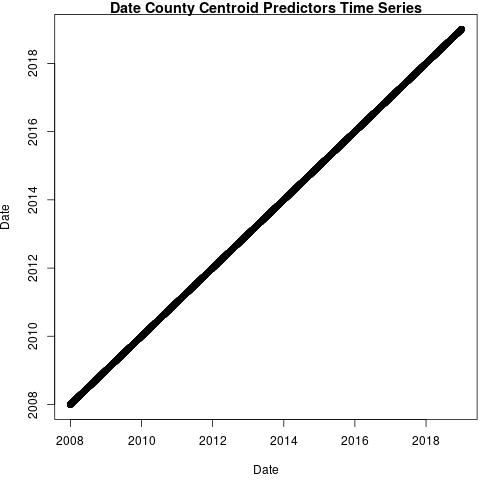
\includegraphics[width=0.77\textwidth]{Code_Outputs/df_report_ML_predictors_CountyCentroid_Locations_Dates_2008-01-01to2018-12-31_DatevDate.jpg} 
\caption{\label{fig:df_report_ML_predictors_CountyCentroid_Locations_Dates_2008-01-01to2018-12-31DatevDate}Date County Centroid Predictors Time Series} 
\end{figure} 
 

\begin{figure} 
\centering  
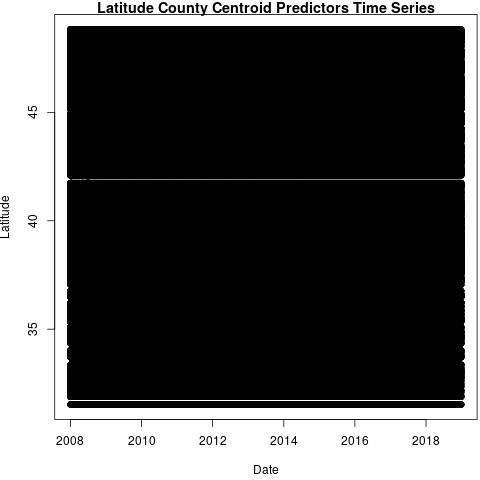
\includegraphics[width=0.77\textwidth]{Code_Outputs/df_report_ML_predictors_CountyCentroid_Locations_Dates_2008-01-01to2018-12-31_LatitudevDate.jpg} 
\caption{\label{fig:df_report_ML_predictors_CountyCentroid_Locations_Dates_2008-01-01to2018-12-31LatitudevDate}Latitude County Centroid Predictors Time Series} 
\end{figure} 
 

\begin{figure} 
\centering  
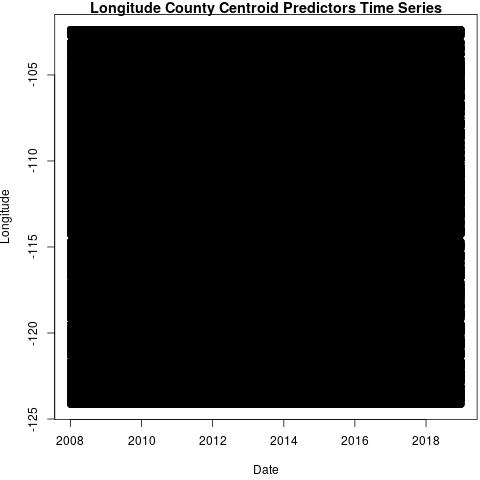
\includegraphics[width=0.77\textwidth]{Code_Outputs/df_report_ML_predictors_CountyCentroid_Locations_Dates_2008-01-01to2018-12-31_LongitudevDate.jpg} 
\caption{\label{fig:df_report_ML_predictors_CountyCentroid_Locations_Dates_2008-01-01to2018-12-31LongitudevDate}Longitude County Centroid Predictors Time Series} 
\end{figure} 
 


\clearpage

\subsection{County Centroid Predictors Map subset of days Images} 
 

\begin{figure} 
\centering  
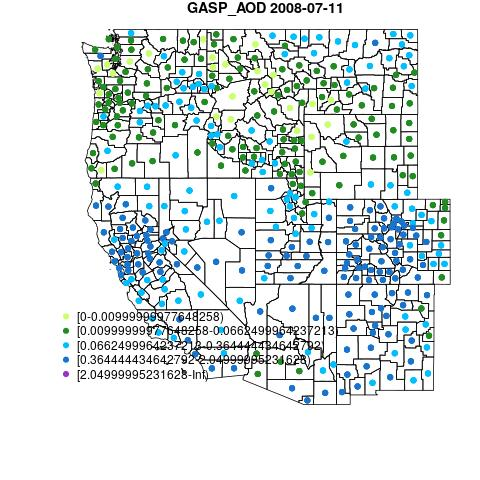
\includegraphics[width=0.77\textwidth]{Code_Outputs/df_report_ML_predictors_CountyCentroid_Locations_Dates_2008-01-01to2018-12-31_MapObsGASP_AOD2008-07-11.jpg} 
\caption{\label{fig:df_report_ML_predictors_CountyCentroid_Locations_Dates_2008-01-01to2018-12-31MapObsGASP_AOD2008-07-11}GASP-AOD 2008-07-11} 
\end{figure} 
 

\begin{figure} 
\centering  
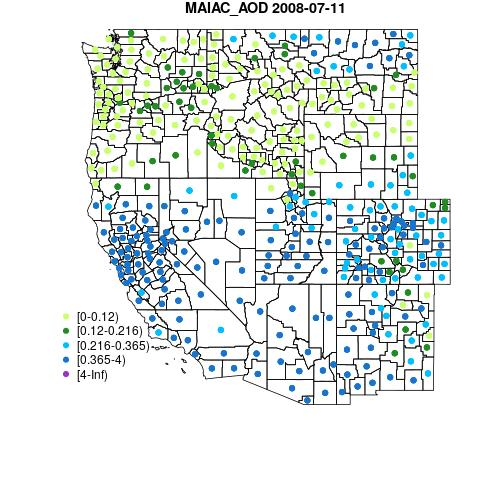
\includegraphics[width=0.77\textwidth]{Code_Outputs/df_report_ML_predictors_CountyCentroid_Locations_Dates_2008-01-01to2018-12-31_MapObsMAIAC_AOD2008-07-11.jpg} 
\caption{\label{fig:df_report_ML_predictors_CountyCentroid_Locations_Dates_2008-01-01to2018-12-31MapObsMAIAC_AOD2008-07-11}MAIAC-AOD 2008-07-11} 
\end{figure} 
 

\begin{figure} 
\centering  
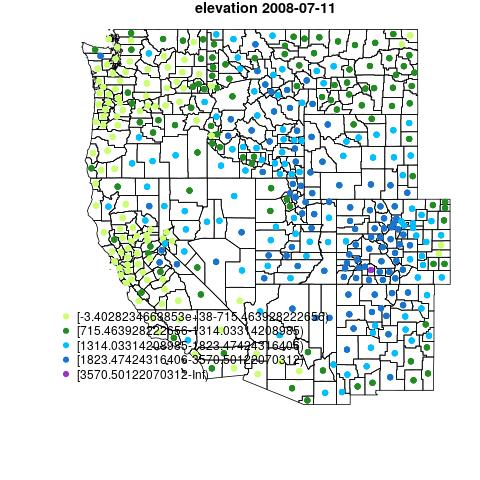
\includegraphics[width=0.77\textwidth]{Code_Outputs/df_report_ML_predictors_CountyCentroid_Locations_Dates_2008-01-01to2018-12-31_MapObselevation2008-07-11.jpg} 
\caption{\label{fig:df_report_ML_predictors_CountyCentroid_Locations_Dates_2008-01-01to2018-12-31MapObselevation2008-07-11}elevation 2008-07-11} 
\end{figure} 
 

\begin{figure} 
\centering  
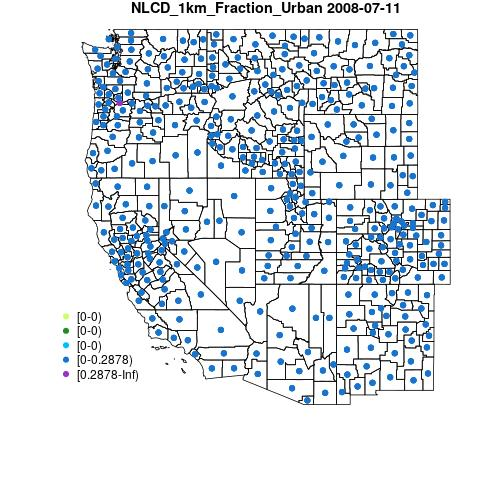
\includegraphics[width=0.77\textwidth]{Code_Outputs/df_report_ML_predictors_CountyCentroid_Locations_Dates_2008-01-01to2018-12-31_MapObsNLCD_1km_Fraction_Urban2008-07-11.jpg} 
\caption{\label{fig:df_report_ML_predictors_CountyCentroid_Locations_Dates_2008-01-01to2018-12-31MapObsNLCD_1km_Fraction_Urban2008-07-11}NLCD-1km-Fraction-Urban 2008-07-11} 
\end{figure} 
 

\begin{figure} 
\centering  
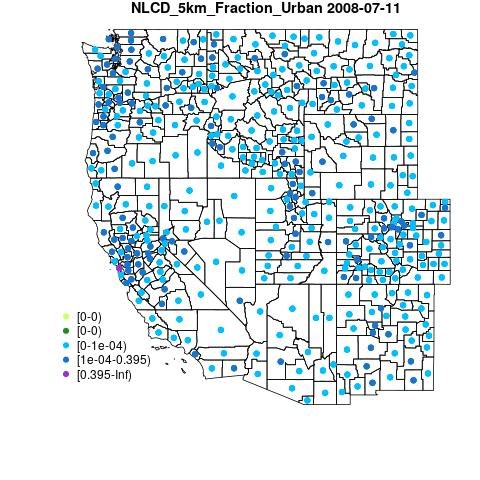
\includegraphics[width=0.77\textwidth]{Code_Outputs/df_report_ML_predictors_CountyCentroid_Locations_Dates_2008-01-01to2018-12-31_MapObsNLCD_5km_Fraction_Urban2008-07-11.jpg} 
\caption{\label{fig:df_report_ML_predictors_CountyCentroid_Locations_Dates_2008-01-01to2018-12-31MapObsNLCD_5km_Fraction_Urban2008-07-11}NLCD-5km-Fraction-Urban 2008-07-11} 
\end{figure} 
 

\begin{figure} 
\centering  
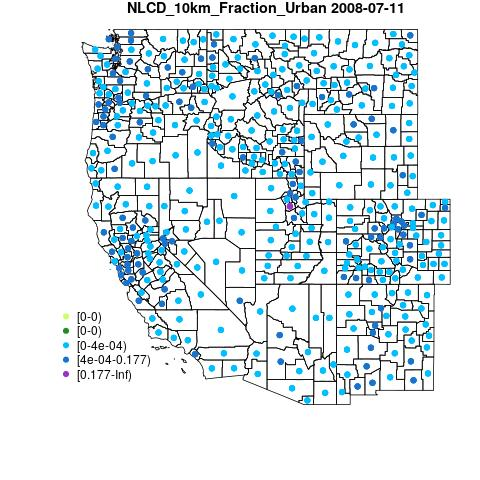
\includegraphics[width=0.77\textwidth]{Code_Outputs/df_report_ML_predictors_CountyCentroid_Locations_Dates_2008-01-01to2018-12-31_MapObsNLCD_10km_Fraction_Urban2008-07-11.jpg} 
\caption{\label{fig:df_report_ML_predictors_CountyCentroid_Locations_Dates_2008-01-01to2018-12-31MapObsNLCD_10km_Fraction_Urban2008-07-11}NLCD-10km-Fraction-Urban 2008-07-11} 
\end{figure} 
 

\begin{figure} 
\centering  
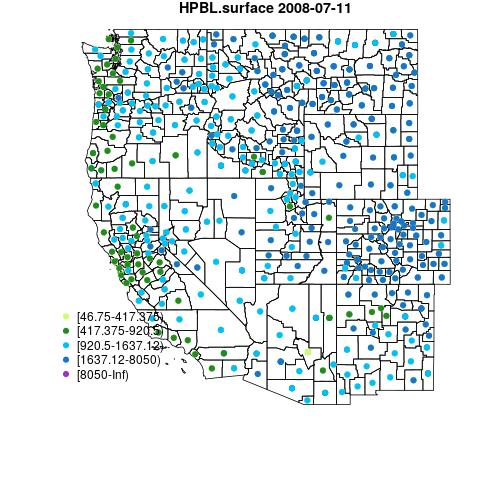
\includegraphics[width=0.77\textwidth]{Code_Outputs/df_report_ML_predictors_CountyCentroid_Locations_Dates_2008-01-01to2018-12-31_MapObsHPBLsurface2008-07-11.jpg} 
\caption{\label{fig:df_report_ML_predictors_CountyCentroid_Locations_Dates_2008-01-01to2018-12-31MapObsHPBLsurface2008-07-11}HPBL.surface 2008-07-11} 
\end{figure} 
 

\begin{figure} 
\centering  
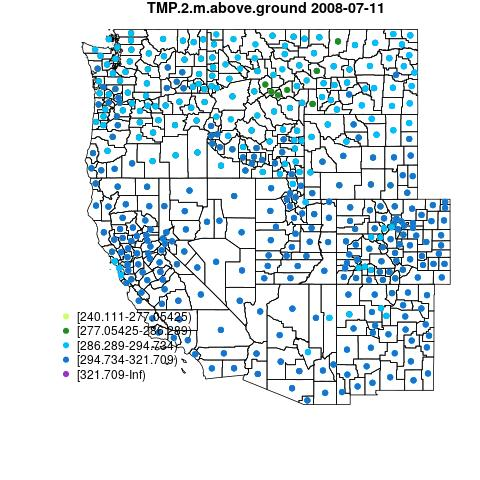
\includegraphics[width=0.77\textwidth]{Code_Outputs/df_report_ML_predictors_CountyCentroid_Locations_Dates_2008-01-01to2018-12-31_MapObsTMP2maboveground2008-07-11.jpg} 
\caption{\label{fig:df_report_ML_predictors_CountyCentroid_Locations_Dates_2008-01-01to2018-12-31MapObsTMP2maboveground2008-07-11}TMP.2.m.above.ground 2008-07-11} 
\end{figure} 
 

\begin{figure} 
\centering  
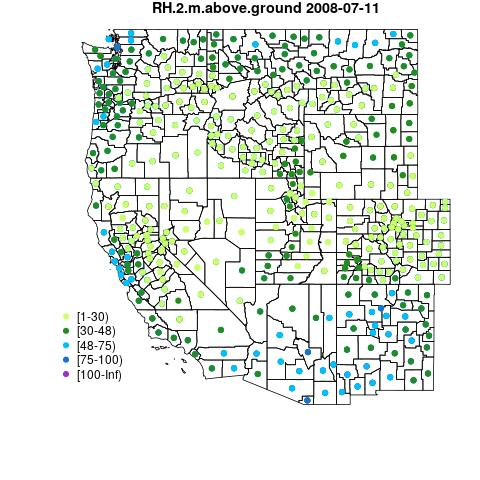
\includegraphics[width=0.77\textwidth]{Code_Outputs/df_report_ML_predictors_CountyCentroid_Locations_Dates_2008-01-01to2018-12-31_MapObsRH2maboveground2008-07-11.jpg} 
\caption{\label{fig:df_report_ML_predictors_CountyCentroid_Locations_Dates_2008-01-01to2018-12-31MapObsRH2maboveground2008-07-11}RH.2.m.above.ground 2008-07-11} 
\end{figure} 
 

\clearpage 

\begin{figure} 
\centering  
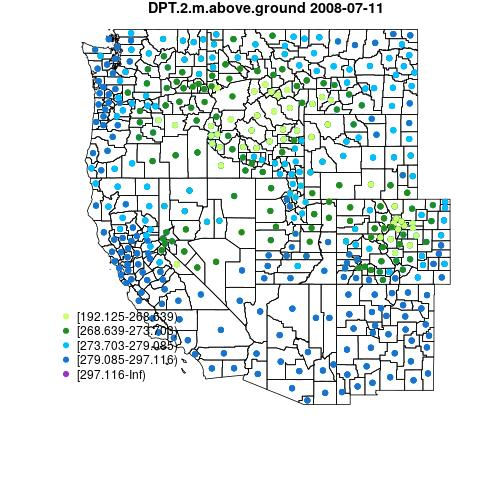
\includegraphics[width=0.77\textwidth]{Code_Outputs/df_report_ML_predictors_CountyCentroid_Locations_Dates_2008-01-01to2018-12-31_MapObsDPT2maboveground2008-07-11.jpg} 
\caption{\label{fig:df_report_ML_predictors_CountyCentroid_Locations_Dates_2008-01-01to2018-12-31MapObsDPT2maboveground2008-07-11}DPT.2.m.above.ground 2008-07-11} 
\end{figure} 
 

\begin{figure} 
\centering  
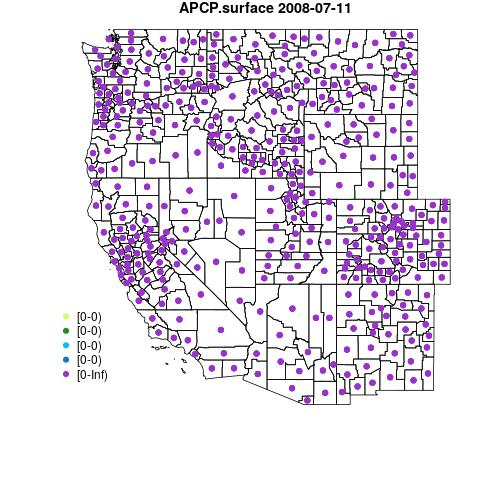
\includegraphics[width=0.77\textwidth]{Code_Outputs/df_report_ML_predictors_CountyCentroid_Locations_Dates_2008-01-01to2018-12-31_MapObsAPCPsurface2008-07-11.jpg} 
\caption{\label{fig:df_report_ML_predictors_CountyCentroid_Locations_Dates_2008-01-01to2018-12-31MapObsAPCPsurface2008-07-11}APCP.surface 2008-07-11} 
\end{figure} 
 

\begin{figure} 
\centering  
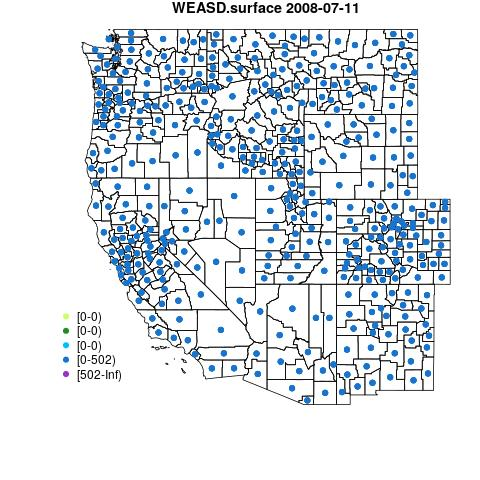
\includegraphics[width=0.77\textwidth]{Code_Outputs/df_report_ML_predictors_CountyCentroid_Locations_Dates_2008-01-01to2018-12-31_MapObsWEASDsurface2008-07-11.jpg} 
\caption{\label{fig:df_report_ML_predictors_CountyCentroid_Locations_Dates_2008-01-01to2018-12-31MapObsWEASDsurface2008-07-11}WEASD.surface 2008-07-11} 
\end{figure} 
 

\begin{figure} 
\centering  
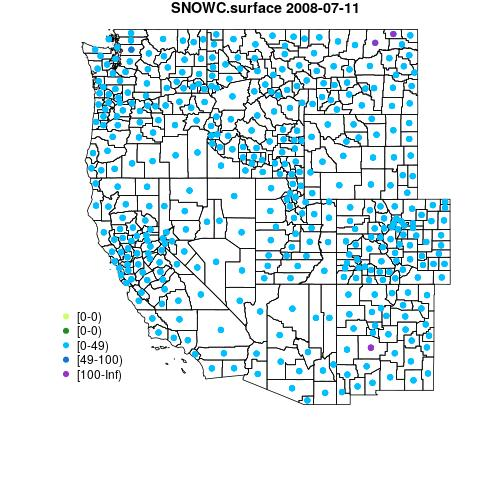
\includegraphics[width=0.77\textwidth]{Code_Outputs/df_report_ML_predictors_CountyCentroid_Locations_Dates_2008-01-01to2018-12-31_MapObsSNOWCsurface2008-07-11.jpg} 
\caption{\label{fig:df_report_ML_predictors_CountyCentroid_Locations_Dates_2008-01-01to2018-12-31MapObsSNOWCsurface2008-07-11}SNOWC.surface 2008-07-11} 
\end{figure} 
 

\begin{figure} 
\centering  
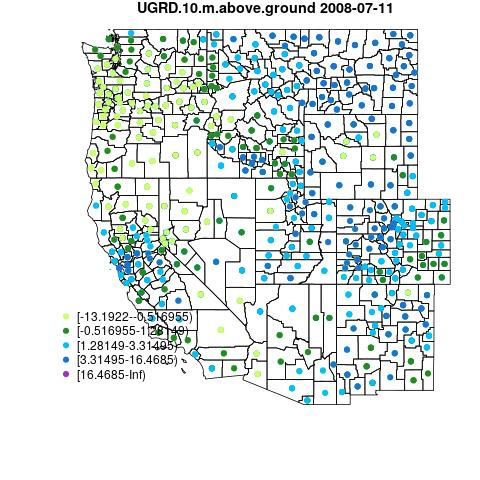
\includegraphics[width=0.77\textwidth]{Code_Outputs/df_report_ML_predictors_CountyCentroid_Locations_Dates_2008-01-01to2018-12-31_MapObsUGRD10maboveground2008-07-11.jpg} 
\caption{\label{fig:df_report_ML_predictors_CountyCentroid_Locations_Dates_2008-01-01to2018-12-31MapObsUGRD10maboveground2008-07-11}UGRD.10.m.above.ground 2008-07-11} 
\end{figure} 
 

\begin{figure} 
\centering  
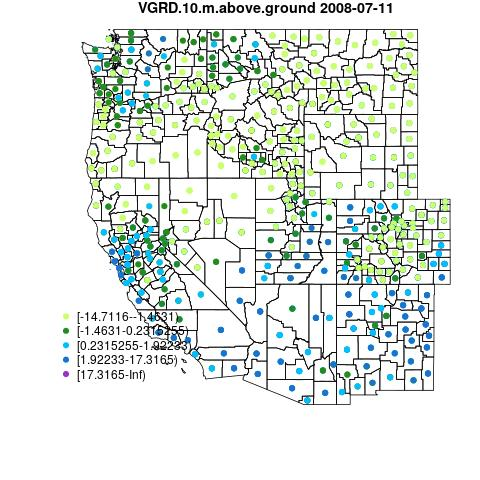
\includegraphics[width=0.77\textwidth]{Code_Outputs/df_report_ML_predictors_CountyCentroid_Locations_Dates_2008-01-01to2018-12-31_MapObsVGRD10maboveground2008-07-11.jpg} 
\caption{\label{fig:df_report_ML_predictors_CountyCentroid_Locations_Dates_2008-01-01to2018-12-31MapObsVGRD10maboveground2008-07-11}VGRD.10.m.above.ground 2008-07-11} 
\end{figure} 
 

\begin{figure} 
\centering  
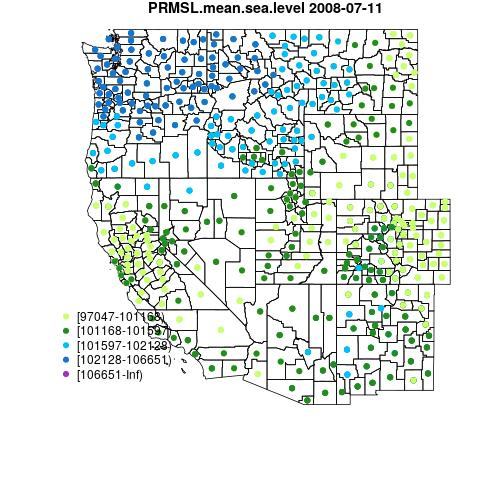
\includegraphics[width=0.77\textwidth]{Code_Outputs/df_report_ML_predictors_CountyCentroid_Locations_Dates_2008-01-01to2018-12-31_MapObsPRMSLmeansealevel2008-07-11.jpg} 
\caption{\label{fig:df_report_ML_predictors_CountyCentroid_Locations_Dates_2008-01-01to2018-12-31MapObsPRMSLmeansealevel2008-07-11}PRMSL.mean.sea.level 2008-07-11} 
\end{figure} 
 

\begin{figure} 
\centering  
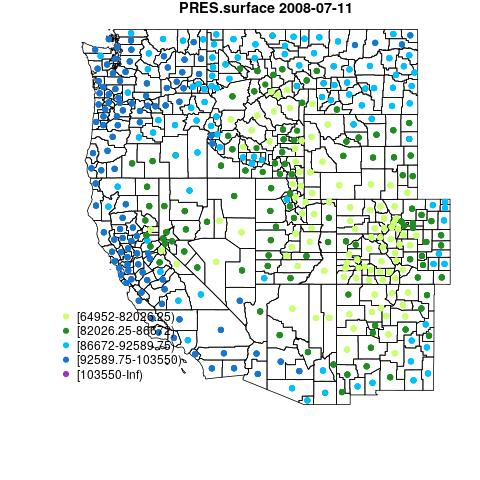
\includegraphics[width=0.77\textwidth]{Code_Outputs/df_report_ML_predictors_CountyCentroid_Locations_Dates_2008-01-01to2018-12-31_MapObsPRESsurface2008-07-11.jpg} 
\caption{\label{fig:df_report_ML_predictors_CountyCentroid_Locations_Dates_2008-01-01to2018-12-31MapObsPRESsurface2008-07-11}PRES.surface 2008-07-11} 
\end{figure} 
 

\begin{figure} 
\centering  
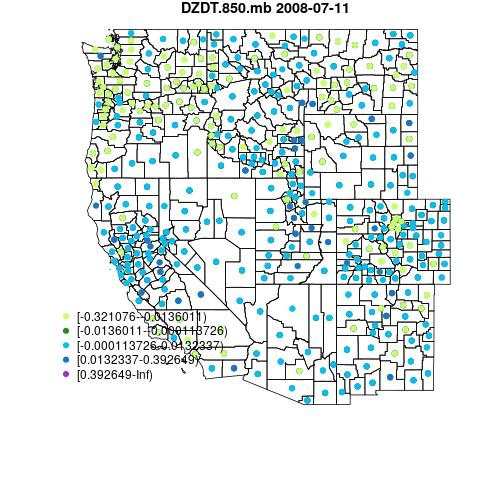
\includegraphics[width=0.77\textwidth]{Code_Outputs/df_report_ML_predictors_CountyCentroid_Locations_Dates_2008-01-01to2018-12-31_MapObsDZDT850mb2008-07-11.jpg} 
\caption{\label{fig:df_report_ML_predictors_CountyCentroid_Locations_Dates_2008-01-01to2018-12-31MapObsDZDT850mb2008-07-11}DZDT.850.mb 2008-07-11} 
\end{figure} 
 

\begin{figure} 
\centering  
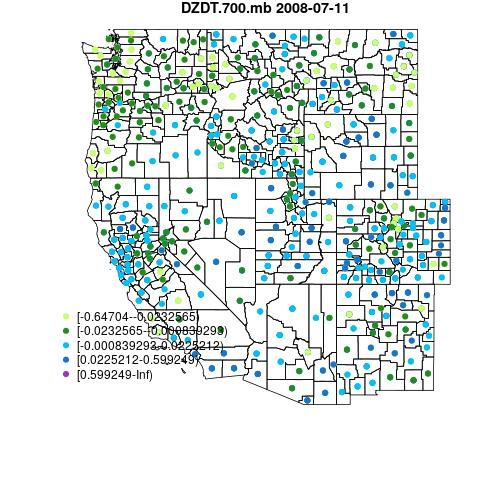
\includegraphics[width=0.77\textwidth]{Code_Outputs/df_report_ML_predictors_CountyCentroid_Locations_Dates_2008-01-01to2018-12-31_MapObsDZDT700mb2008-07-11.jpg} 
\caption{\label{fig:df_report_ML_predictors_CountyCentroid_Locations_Dates_2008-01-01to2018-12-31MapObsDZDT700mb2008-07-11}DZDT.700.mb 2008-07-11} 
\end{figure} 
 

\clearpage 

\begin{figure} 
\centering  
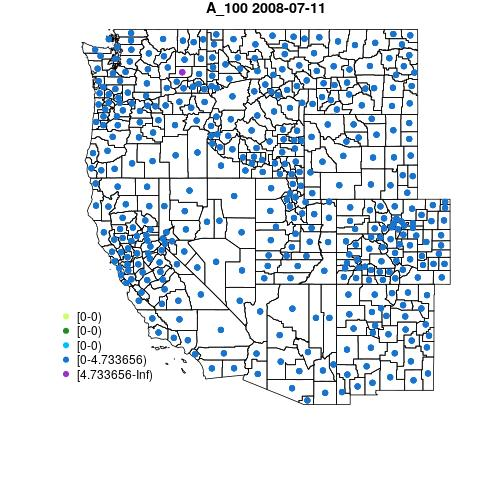
\includegraphics[width=0.77\textwidth]{Code_Outputs/df_report_ML_predictors_CountyCentroid_Locations_Dates_2008-01-01to2018-12-31_MapObsA_1002008-07-11.jpg} 
\caption{\label{fig:df_report_ML_predictors_CountyCentroid_Locations_Dates_2008-01-01to2018-12-31MapObsA_1002008-07-11}A-100 2008-07-11} 
\end{figure} 
 

\begin{figure} 
\centering  
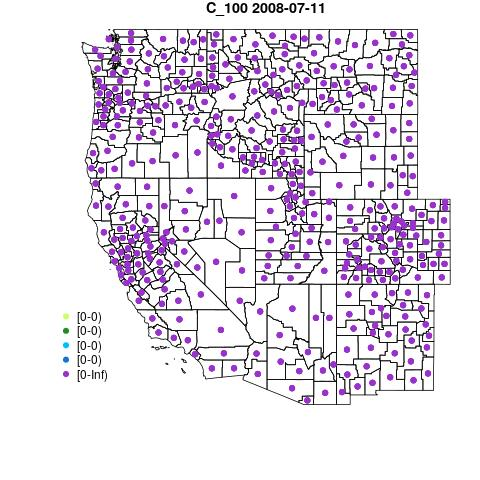
\includegraphics[width=0.77\textwidth]{Code_Outputs/df_report_ML_predictors_CountyCentroid_Locations_Dates_2008-01-01to2018-12-31_MapObsC_1002008-07-11.jpg} 
\caption{\label{fig:df_report_ML_predictors_CountyCentroid_Locations_Dates_2008-01-01to2018-12-31MapObsC_1002008-07-11}C-100 2008-07-11} 
\end{figure} 
 

\begin{figure} 
\centering  
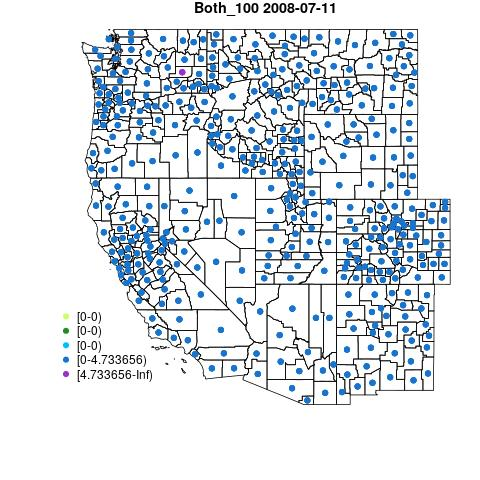
\includegraphics[width=0.77\textwidth]{Code_Outputs/df_report_ML_predictors_CountyCentroid_Locations_Dates_2008-01-01to2018-12-31_MapObsBoth_1002008-07-11.jpg} 
\caption{\label{fig:df_report_ML_predictors_CountyCentroid_Locations_Dates_2008-01-01to2018-12-31MapObsBoth_1002008-07-11}Both-100 2008-07-11} 
\end{figure} 
 

\begin{figure} 
\centering  
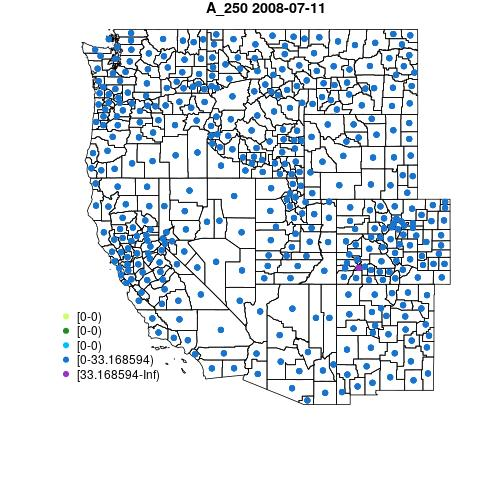
\includegraphics[width=0.77\textwidth]{Code_Outputs/df_report_ML_predictors_CountyCentroid_Locations_Dates_2008-01-01to2018-12-31_MapObsA_2502008-07-11.jpg} 
\caption{\label{fig:df_report_ML_predictors_CountyCentroid_Locations_Dates_2008-01-01to2018-12-31MapObsA_2502008-07-11}A-250 2008-07-11} 
\end{figure} 
 

\begin{figure} 
\centering  
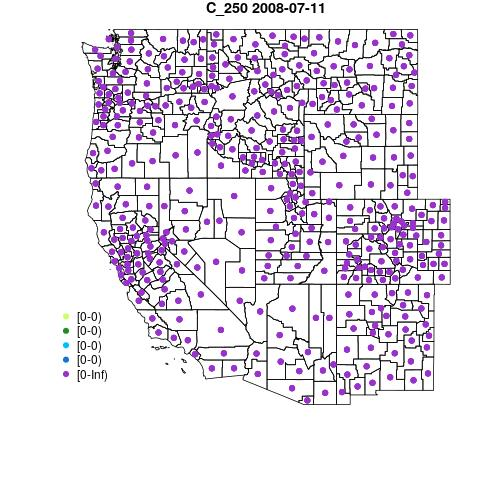
\includegraphics[width=0.77\textwidth]{Code_Outputs/df_report_ML_predictors_CountyCentroid_Locations_Dates_2008-01-01to2018-12-31_MapObsC_2502008-07-11.jpg} 
\caption{\label{fig:df_report_ML_predictors_CountyCentroid_Locations_Dates_2008-01-01to2018-12-31MapObsC_2502008-07-11}C-250 2008-07-11} 
\end{figure} 
 

\begin{figure} 
\centering  
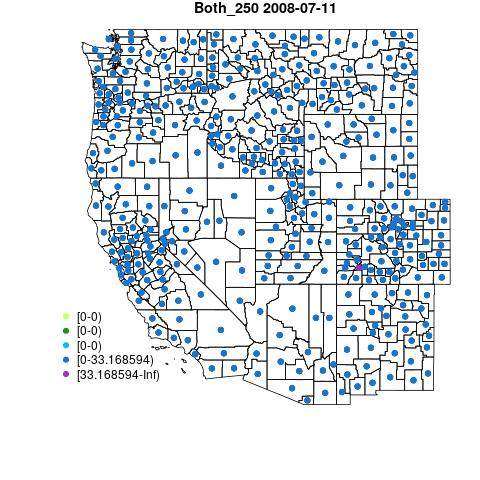
\includegraphics[width=0.77\textwidth]{Code_Outputs/df_report_ML_predictors_CountyCentroid_Locations_Dates_2008-01-01to2018-12-31_MapObsBoth_2502008-07-11.jpg} 
\caption{\label{fig:df_report_ML_predictors_CountyCentroid_Locations_Dates_2008-01-01to2018-12-31MapObsBoth_2502008-07-11}Both-250 2008-07-11} 
\end{figure} 
 

\begin{figure} 
\centering  
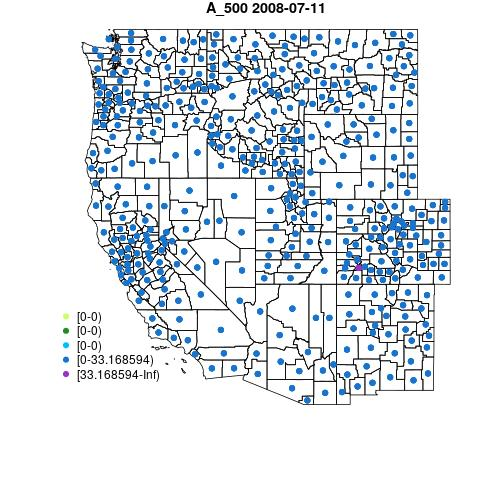
\includegraphics[width=0.77\textwidth]{Code_Outputs/df_report_ML_predictors_CountyCentroid_Locations_Dates_2008-01-01to2018-12-31_MapObsA_5002008-07-11.jpg} 
\caption{\label{fig:df_report_ML_predictors_CountyCentroid_Locations_Dates_2008-01-01to2018-12-31MapObsA_5002008-07-11}A-500 2008-07-11} 
\end{figure} 
 

\begin{figure} 
\centering  
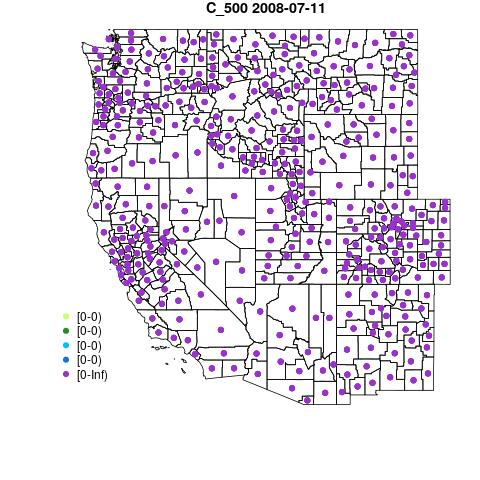
\includegraphics[width=0.77\textwidth]{Code_Outputs/df_report_ML_predictors_CountyCentroid_Locations_Dates_2008-01-01to2018-12-31_MapObsC_5002008-07-11.jpg} 
\caption{\label{fig:df_report_ML_predictors_CountyCentroid_Locations_Dates_2008-01-01to2018-12-31MapObsC_5002008-07-11}C-500 2008-07-11} 
\end{figure} 
 

\begin{figure} 
\centering  
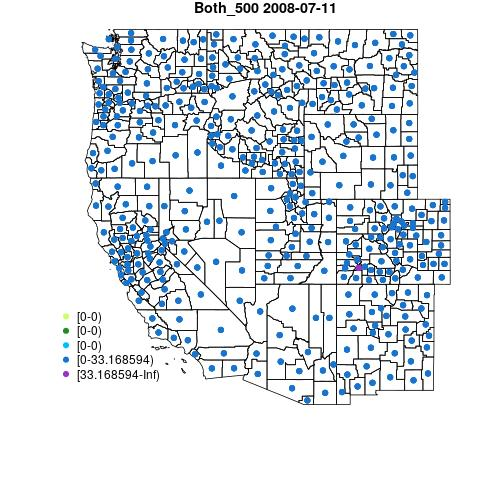
\includegraphics[width=0.77\textwidth]{Code_Outputs/df_report_ML_predictors_CountyCentroid_Locations_Dates_2008-01-01to2018-12-31_MapObsBoth_5002008-07-11.jpg} 
\caption{\label{fig:df_report_ML_predictors_CountyCentroid_Locations_Dates_2008-01-01to2018-12-31MapObsBoth_5002008-07-11}Both-500 2008-07-11} 
\end{figure} 
 

\begin{figure} 
\centering  
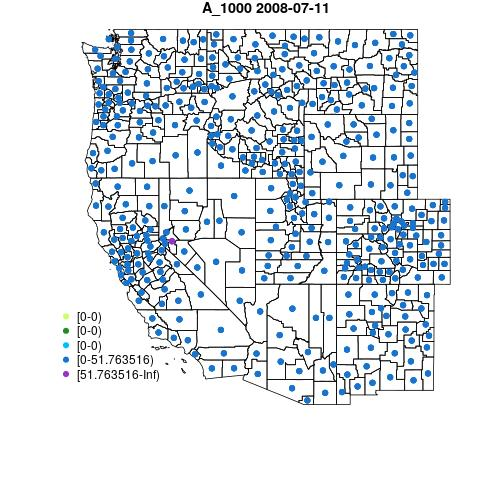
\includegraphics[width=0.77\textwidth]{Code_Outputs/df_report_ML_predictors_CountyCentroid_Locations_Dates_2008-01-01to2018-12-31_MapObsA_10002008-07-11.jpg} 
\caption{\label{fig:df_report_ML_predictors_CountyCentroid_Locations_Dates_2008-01-01to2018-12-31MapObsA_10002008-07-11}A-1000 2008-07-11} 
\end{figure} 
 

\clearpage 

\begin{figure} 
\centering  
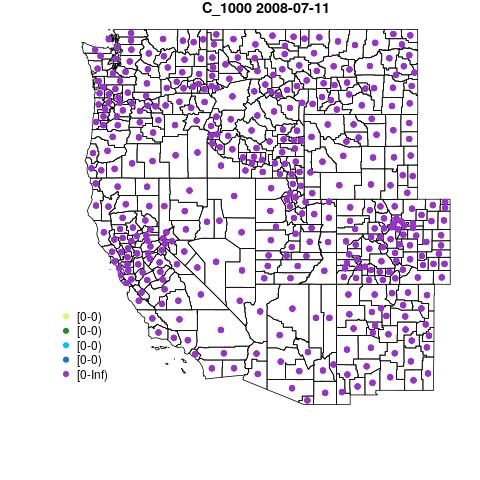
\includegraphics[width=0.77\textwidth]{Code_Outputs/df_report_ML_predictors_CountyCentroid_Locations_Dates_2008-01-01to2018-12-31_MapObsC_10002008-07-11.jpg} 
\caption{\label{fig:df_report_ML_predictors_CountyCentroid_Locations_Dates_2008-01-01to2018-12-31MapObsC_10002008-07-11}C-1000 2008-07-11} 
\end{figure} 
 

\begin{figure} 
\centering  
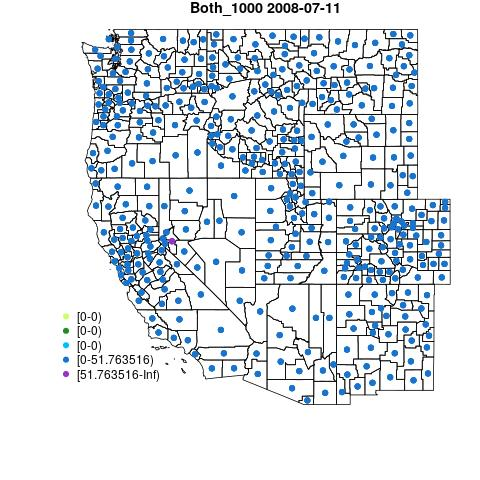
\includegraphics[width=0.77\textwidth]{Code_Outputs/df_report_ML_predictors_CountyCentroid_Locations_Dates_2008-01-01to2018-12-31_MapObsBoth_10002008-07-11.jpg} 
\caption{\label{fig:df_report_ML_predictors_CountyCentroid_Locations_Dates_2008-01-01to2018-12-31MapObsBoth_10002008-07-11}Both-1000 2008-07-11} 
\end{figure} 
 


\clearpage

\subsection{County Centroid Predictors Map monthly medians Images} 
 

\begin{figure} 
\centering  
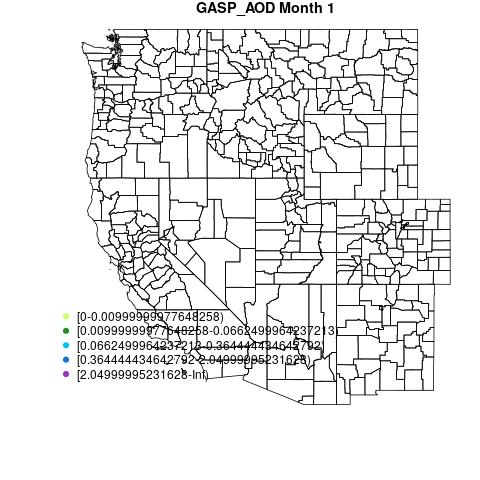
\includegraphics[width=0.77\textwidth]{Code_Outputs/df_report_ML_predictors_CountyCentroid_Locations_Dates_2008-01-01to2018-12-31_MapObsMo1GASP_AOD.jpg} 
\caption{\label{fig:df_report_ML_predictors_CountyCentroid_Locations_Dates_2008-01-01to2018-12-31MapObsMo1GASP_AOD}GASP-AOD Month 1} 
\end{figure} 
 

\begin{figure} 
\centering  
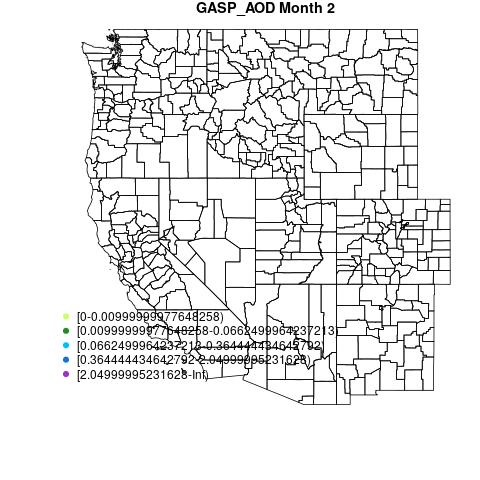
\includegraphics[width=0.77\textwidth]{Code_Outputs/df_report_ML_predictors_CountyCentroid_Locations_Dates_2008-01-01to2018-12-31_MapObsMo2GASP_AOD.jpg} 
\caption{\label{fig:df_report_ML_predictors_CountyCentroid_Locations_Dates_2008-01-01to2018-12-31MapObsMo2GASP_AOD}GASP-AOD Month 2} 
\end{figure} 
 

\begin{figure} 
\centering  
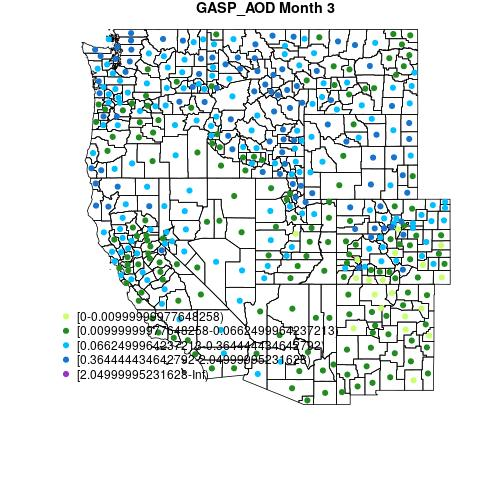
\includegraphics[width=0.77\textwidth]{Code_Outputs/df_report_ML_predictors_CountyCentroid_Locations_Dates_2008-01-01to2018-12-31_MapObsMo3GASP_AOD.jpg} 
\caption{\label{fig:df_report_ML_predictors_CountyCentroid_Locations_Dates_2008-01-01to2018-12-31MapObsMo3GASP_AOD}GASP-AOD Month 3} 
\end{figure} 
 

\begin{figure} 
\centering  
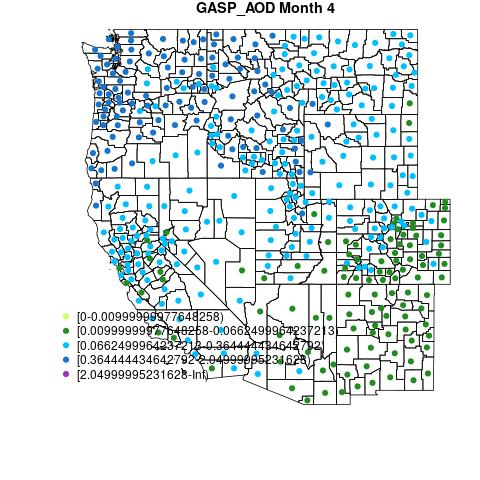
\includegraphics[width=0.77\textwidth]{Code_Outputs/df_report_ML_predictors_CountyCentroid_Locations_Dates_2008-01-01to2018-12-31_MapObsMo4GASP_AOD.jpg} 
\caption{\label{fig:df_report_ML_predictors_CountyCentroid_Locations_Dates_2008-01-01to2018-12-31MapObsMo4GASP_AOD}GASP-AOD Month 4} 
\end{figure} 
 

\begin{figure} 
\centering  
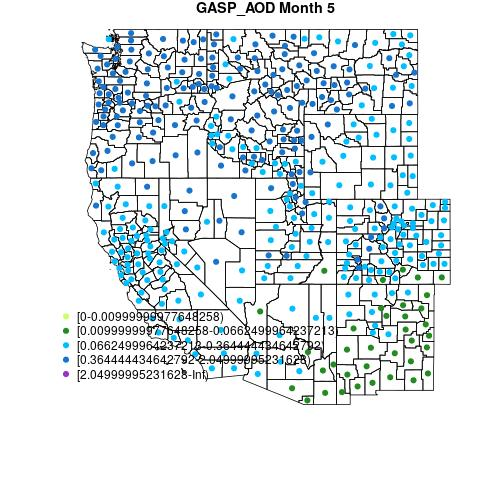
\includegraphics[width=0.77\textwidth]{Code_Outputs/df_report_ML_predictors_CountyCentroid_Locations_Dates_2008-01-01to2018-12-31_MapObsMo5GASP_AOD.jpg} 
\caption{\label{fig:df_report_ML_predictors_CountyCentroid_Locations_Dates_2008-01-01to2018-12-31MapObsMo5GASP_AOD}GASP-AOD Month 5} 
\end{figure} 
 

\begin{figure} 
\centering  
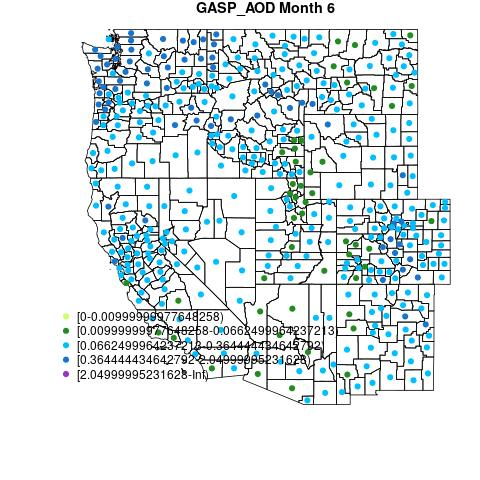
\includegraphics[width=0.77\textwidth]{Code_Outputs/df_report_ML_predictors_CountyCentroid_Locations_Dates_2008-01-01to2018-12-31_MapObsMo6GASP_AOD.jpg} 
\caption{\label{fig:df_report_ML_predictors_CountyCentroid_Locations_Dates_2008-01-01to2018-12-31MapObsMo6GASP_AOD}GASP-AOD Month 6} 
\end{figure} 
 

\begin{figure} 
\centering  
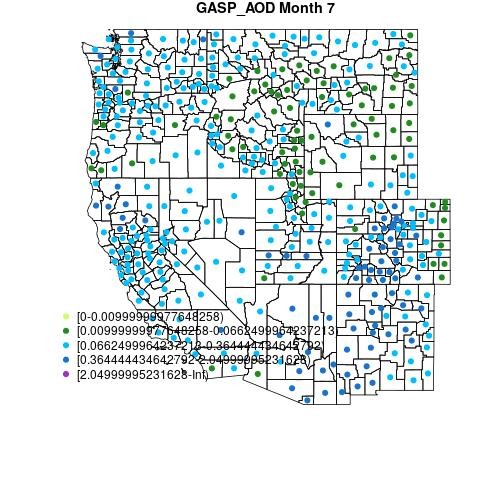
\includegraphics[width=0.77\textwidth]{Code_Outputs/df_report_ML_predictors_CountyCentroid_Locations_Dates_2008-01-01to2018-12-31_MapObsMo7GASP_AOD.jpg} 
\caption{\label{fig:df_report_ML_predictors_CountyCentroid_Locations_Dates_2008-01-01to2018-12-31MapObsMo7GASP_AOD}GASP-AOD Month 7} 
\end{figure} 
 

\begin{figure} 
\centering  
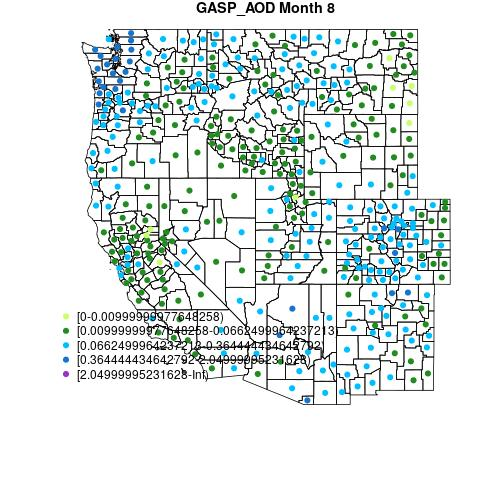
\includegraphics[width=0.77\textwidth]{Code_Outputs/df_report_ML_predictors_CountyCentroid_Locations_Dates_2008-01-01to2018-12-31_MapObsMo8GASP_AOD.jpg} 
\caption{\label{fig:df_report_ML_predictors_CountyCentroid_Locations_Dates_2008-01-01to2018-12-31MapObsMo8GASP_AOD}GASP-AOD Month 8} 
\end{figure} 
 

\begin{figure} 
\centering  
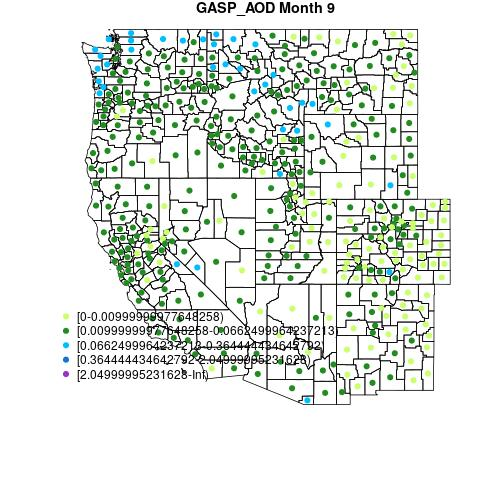
\includegraphics[width=0.77\textwidth]{Code_Outputs/df_report_ML_predictors_CountyCentroid_Locations_Dates_2008-01-01to2018-12-31_MapObsMo9GASP_AOD.jpg} 
\caption{\label{fig:df_report_ML_predictors_CountyCentroid_Locations_Dates_2008-01-01to2018-12-31MapObsMo9GASP_AOD}GASP-AOD Month 9} 
\end{figure} 
 

\clearpage 

\begin{figure} 
\centering  
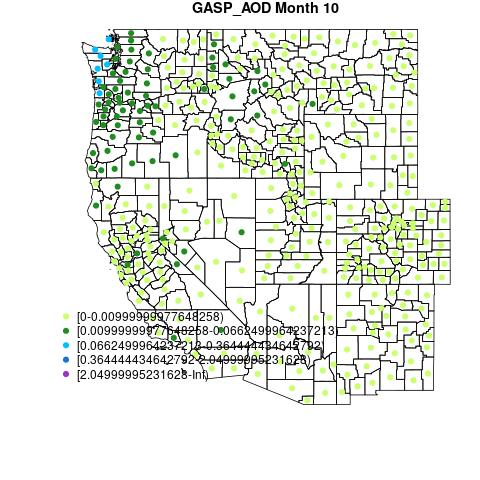
\includegraphics[width=0.77\textwidth]{Code_Outputs/df_report_ML_predictors_CountyCentroid_Locations_Dates_2008-01-01to2018-12-31_MapObsMo10GASP_AOD.jpg} 
\caption{\label{fig:df_report_ML_predictors_CountyCentroid_Locations_Dates_2008-01-01to2018-12-31MapObsMo10GASP_AOD}GASP-AOD Month 10} 
\end{figure} 
 

\begin{figure} 
\centering  
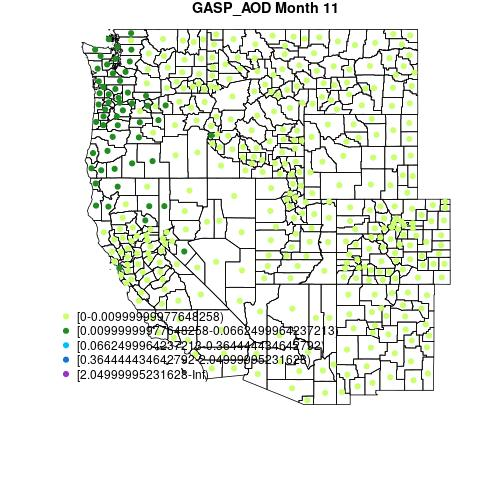
\includegraphics[width=0.77\textwidth]{Code_Outputs/df_report_ML_predictors_CountyCentroid_Locations_Dates_2008-01-01to2018-12-31_MapObsMo11GASP_AOD.jpg} 
\caption{\label{fig:df_report_ML_predictors_CountyCentroid_Locations_Dates_2008-01-01to2018-12-31MapObsMo11GASP_AOD}GASP-AOD Month 11} 
\end{figure} 
 

\begin{figure} 
\centering  
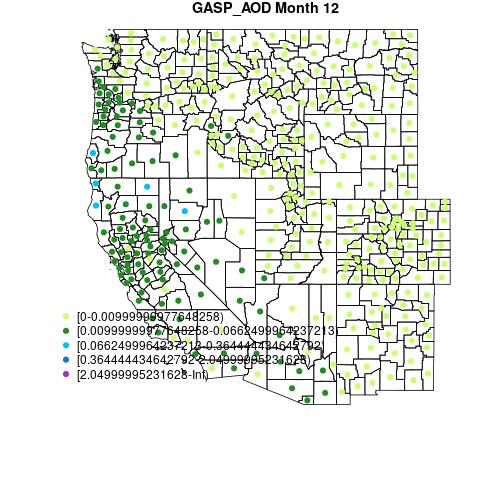
\includegraphics[width=0.77\textwidth]{Code_Outputs/df_report_ML_predictors_CountyCentroid_Locations_Dates_2008-01-01to2018-12-31_MapObsMo12GASP_AOD.jpg} 
\caption{\label{fig:df_report_ML_predictors_CountyCentroid_Locations_Dates_2008-01-01to2018-12-31MapObsMo12GASP_AOD}GASP-AOD Month 12} 
\end{figure} 
 

\begin{figure} 
\centering  
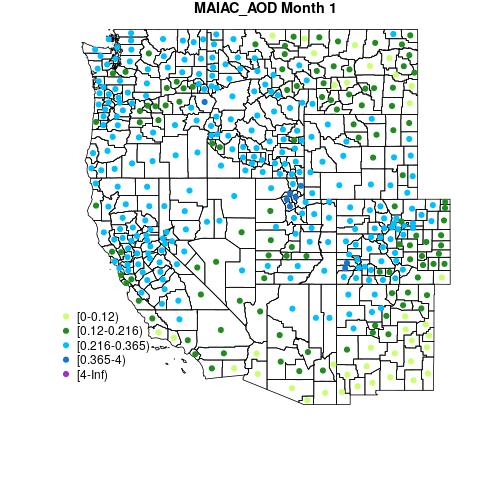
\includegraphics[width=0.77\textwidth]{Code_Outputs/df_report_ML_predictors_CountyCentroid_Locations_Dates_2008-01-01to2018-12-31_MapObsMo1MAIAC_AOD.jpg} 
\caption{\label{fig:df_report_ML_predictors_CountyCentroid_Locations_Dates_2008-01-01to2018-12-31MapObsMo1MAIAC_AOD}MAIAC-AOD Month 1} 
\end{figure} 
 

\begin{figure} 
\centering  
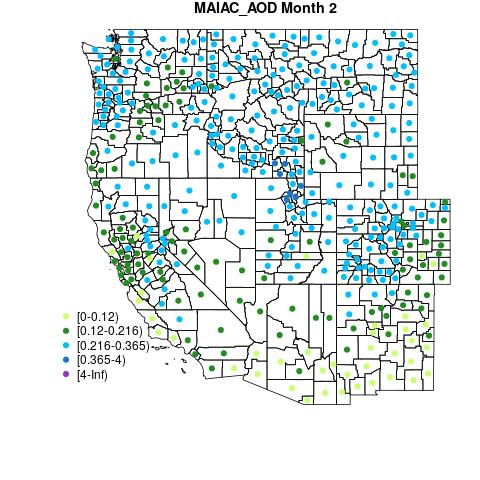
\includegraphics[width=0.77\textwidth]{Code_Outputs/df_report_ML_predictors_CountyCentroid_Locations_Dates_2008-01-01to2018-12-31_MapObsMo2MAIAC_AOD.jpg} 
\caption{\label{fig:df_report_ML_predictors_CountyCentroid_Locations_Dates_2008-01-01to2018-12-31MapObsMo2MAIAC_AOD}MAIAC-AOD Month 2} 
\end{figure} 
 

\begin{figure} 
\centering  
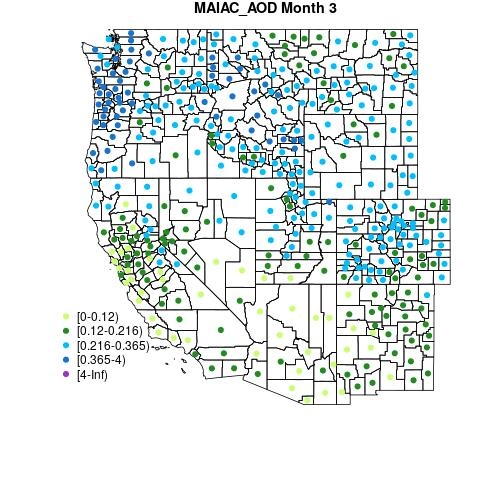
\includegraphics[width=0.77\textwidth]{Code_Outputs/df_report_ML_predictors_CountyCentroid_Locations_Dates_2008-01-01to2018-12-31_MapObsMo3MAIAC_AOD.jpg} 
\caption{\label{fig:df_report_ML_predictors_CountyCentroid_Locations_Dates_2008-01-01to2018-12-31MapObsMo3MAIAC_AOD}MAIAC-AOD Month 3} 
\end{figure} 
 

\begin{figure} 
\centering  
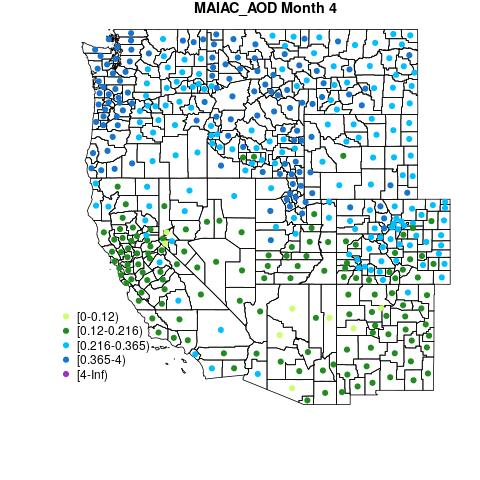
\includegraphics[width=0.77\textwidth]{Code_Outputs/df_report_ML_predictors_CountyCentroid_Locations_Dates_2008-01-01to2018-12-31_MapObsMo4MAIAC_AOD.jpg} 
\caption{\label{fig:df_report_ML_predictors_CountyCentroid_Locations_Dates_2008-01-01to2018-12-31MapObsMo4MAIAC_AOD}MAIAC-AOD Month 4} 
\end{figure} 
 

\begin{figure} 
\centering  
\includegraphics[width=0.77\textwidth]{Code_Outputs/df_report_ML_predictors_CountyCentroid_Locations_Dates_2008-01-01to2018-12-31_MapObsMo5MAIAC_AOD.jpg} 
\caption{\label{fig:df_report_ML_predictors_CountyCentroid_Locations_Dates_2008-01-01to2018-12-31MapObsMo5MAIAC_AOD}MAIAC-AOD Month 5} 
\end{figure} 
 

\begin{figure} 
\centering  
\includegraphics[width=0.77\textwidth]{Code_Outputs/df_report_ML_predictors_CountyCentroid_Locations_Dates_2008-01-01to2018-12-31_MapObsMo6MAIAC_AOD.jpg} 
\caption{\label{fig:df_report_ML_predictors_CountyCentroid_Locations_Dates_2008-01-01to2018-12-31MapObsMo6MAIAC_AOD}MAIAC-AOD Month 6} 
\end{figure} 
 

\begin{figure} 
\centering  
\includegraphics[width=0.77\textwidth]{Code_Outputs/df_report_ML_predictors_CountyCentroid_Locations_Dates_2008-01-01to2018-12-31_MapObsMo7MAIAC_AOD.jpg} 
\caption{\label{fig:df_report_ML_predictors_CountyCentroid_Locations_Dates_2008-01-01to2018-12-31MapObsMo7MAIAC_AOD}MAIAC-AOD Month 7} 
\end{figure} 
 

\clearpage 

\begin{figure} 
\centering  
\includegraphics[width=0.77\textwidth]{Code_Outputs/df_report_ML_predictors_CountyCentroid_Locations_Dates_2008-01-01to2018-12-31_MapObsMo8MAIAC_AOD.jpg} 
\caption{\label{fig:df_report_ML_predictors_CountyCentroid_Locations_Dates_2008-01-01to2018-12-31MapObsMo8MAIAC_AOD}MAIAC-AOD Month 8} 
\end{figure} 
 

\begin{figure} 
\centering  
\includegraphics[width=0.77\textwidth]{Code_Outputs/df_report_ML_predictors_CountyCentroid_Locations_Dates_2008-01-01to2018-12-31_MapObsMo9MAIAC_AOD.jpg} 
\caption{\label{fig:df_report_ML_predictors_CountyCentroid_Locations_Dates_2008-01-01to2018-12-31MapObsMo9MAIAC_AOD}MAIAC-AOD Month 9} 
\end{figure} 
 

\begin{figure} 
\centering  
\includegraphics[width=0.77\textwidth]{Code_Outputs/df_report_ML_predictors_CountyCentroid_Locations_Dates_2008-01-01to2018-12-31_MapObsMo10MAIAC_AOD.jpg} 
\caption{\label{fig:df_report_ML_predictors_CountyCentroid_Locations_Dates_2008-01-01to2018-12-31MapObsMo10MAIAC_AOD}MAIAC-AOD Month 10} 
\end{figure} 
 

\begin{figure} 
\centering  
\includegraphics[width=0.77\textwidth]{Code_Outputs/df_report_ML_predictors_CountyCentroid_Locations_Dates_2008-01-01to2018-12-31_MapObsMo11MAIAC_AOD.jpg} 
\caption{\label{fig:df_report_ML_predictors_CountyCentroid_Locations_Dates_2008-01-01to2018-12-31MapObsMo11MAIAC_AOD}MAIAC-AOD Month 11} 
\end{figure} 
 

\begin{figure} 
\centering  
\includegraphics[width=0.77\textwidth]{Code_Outputs/df_report_ML_predictors_CountyCentroid_Locations_Dates_2008-01-01to2018-12-31_MapObsMo12MAIAC_AOD.jpg} 
\caption{\label{fig:df_report_ML_predictors_CountyCentroid_Locations_Dates_2008-01-01to2018-12-31MapObsMo12MAIAC_AOD}MAIAC-AOD Month 12} 
\end{figure} 
 

\begin{figure} 
\centering  
\includegraphics[width=0.77\textwidth]{Code_Outputs/df_report_ML_predictors_CountyCentroid_Locations_Dates_2008-01-01to2018-12-31_MapObsMo1elevation.jpg} 
\caption{\label{fig:df_report_ML_predictors_CountyCentroid_Locations_Dates_2008-01-01to2018-12-31MapObsMo1elevation}elevation Month 1} 
\end{figure} 
 

\begin{figure} 
\centering  
\includegraphics[width=0.77\textwidth]{Code_Outputs/df_report_ML_predictors_CountyCentroid_Locations_Dates_2008-01-01to2018-12-31_MapObsMo2elevation.jpg} 
\caption{\label{fig:df_report_ML_predictors_CountyCentroid_Locations_Dates_2008-01-01to2018-12-31MapObsMo2elevation}elevation Month 2} 
\end{figure} 
 

\begin{figure} 
\centering  
\includegraphics[width=0.77\textwidth]{Code_Outputs/df_report_ML_predictors_CountyCentroid_Locations_Dates_2008-01-01to2018-12-31_MapObsMo3elevation.jpg} 
\caption{\label{fig:df_report_ML_predictors_CountyCentroid_Locations_Dates_2008-01-01to2018-12-31MapObsMo3elevation}elevation Month 3} 
\end{figure} 
 

\begin{figure} 
\centering  
\includegraphics[width=0.77\textwidth]{Code_Outputs/df_report_ML_predictors_CountyCentroid_Locations_Dates_2008-01-01to2018-12-31_MapObsMo4elevation.jpg} 
\caption{\label{fig:df_report_ML_predictors_CountyCentroid_Locations_Dates_2008-01-01to2018-12-31MapObsMo4elevation}elevation Month 4} 
\end{figure} 
 

\begin{figure} 
\centering  
\includegraphics[width=0.77\textwidth]{Code_Outputs/df_report_ML_predictors_CountyCentroid_Locations_Dates_2008-01-01to2018-12-31_MapObsMo5elevation.jpg} 
\caption{\label{fig:df_report_ML_predictors_CountyCentroid_Locations_Dates_2008-01-01to2018-12-31MapObsMo5elevation}elevation Month 5} 
\end{figure} 
 

\clearpage 

\begin{figure} 
\centering  
\includegraphics[width=0.77\textwidth]{Code_Outputs/df_report_ML_predictors_CountyCentroid_Locations_Dates_2008-01-01to2018-12-31_MapObsMo6elevation.jpg} 
\caption{\label{fig:df_report_ML_predictors_CountyCentroid_Locations_Dates_2008-01-01to2018-12-31MapObsMo6elevation}elevation Month 6} 
\end{figure} 
 

\begin{figure} 
\centering  
\includegraphics[width=0.77\textwidth]{Code_Outputs/df_report_ML_predictors_CountyCentroid_Locations_Dates_2008-01-01to2018-12-31_MapObsMo7elevation.jpg} 
\caption{\label{fig:df_report_ML_predictors_CountyCentroid_Locations_Dates_2008-01-01to2018-12-31MapObsMo7elevation}elevation Month 7} 
\end{figure} 
 

\begin{figure} 
\centering  
\includegraphics[width=0.77\textwidth]{Code_Outputs/df_report_ML_predictors_CountyCentroid_Locations_Dates_2008-01-01to2018-12-31_MapObsMo8elevation.jpg} 
\caption{\label{fig:df_report_ML_predictors_CountyCentroid_Locations_Dates_2008-01-01to2018-12-31MapObsMo8elevation}elevation Month 8} 
\end{figure} 
 

\begin{figure} 
\centering  
\includegraphics[width=0.77\textwidth]{Code_Outputs/df_report_ML_predictors_CountyCentroid_Locations_Dates_2008-01-01to2018-12-31_MapObsMo9elevation.jpg} 
\caption{\label{fig:df_report_ML_predictors_CountyCentroid_Locations_Dates_2008-01-01to2018-12-31MapObsMo9elevation}elevation Month 9} 
\end{figure} 
 

\begin{figure} 
\centering  
\includegraphics[width=0.77\textwidth]{Code_Outputs/df_report_ML_predictors_CountyCentroid_Locations_Dates_2008-01-01to2018-12-31_MapObsMo10elevation.jpg} 
\caption{\label{fig:df_report_ML_predictors_CountyCentroid_Locations_Dates_2008-01-01to2018-12-31MapObsMo10elevation}elevation Month 10} 
\end{figure} 
 

\begin{figure} 
\centering  
\includegraphics[width=0.77\textwidth]{Code_Outputs/df_report_ML_predictors_CountyCentroid_Locations_Dates_2008-01-01to2018-12-31_MapObsMo11elevation.jpg} 
\caption{\label{fig:df_report_ML_predictors_CountyCentroid_Locations_Dates_2008-01-01to2018-12-31MapObsMo11elevation}elevation Month 11} 
\end{figure} 
 

\begin{figure} 
\centering  
\includegraphics[width=0.77\textwidth]{Code_Outputs/df_report_ML_predictors_CountyCentroid_Locations_Dates_2008-01-01to2018-12-31_MapObsMo12elevation.jpg} 
\caption{\label{fig:df_report_ML_predictors_CountyCentroid_Locations_Dates_2008-01-01to2018-12-31MapObsMo12elevation}elevation Month 12} 
\end{figure} 
 

\begin{figure} 
\centering  
\includegraphics[width=0.77\textwidth]{Code_Outputs/df_report_ML_predictors_CountyCentroid_Locations_Dates_2008-01-01to2018-12-31_MapObsMo1NLCD_1km_Fraction_Urban.jpg} 
\caption{\label{fig:df_report_ML_predictors_CountyCentroid_Locations_Dates_2008-01-01to2018-12-31MapObsMo1NLCD_1km_Fraction_Urban}NLCD-1km-Fraction-Urban Month 1} 
\end{figure} 
 

\begin{figure} 
\centering  
\includegraphics[width=0.77\textwidth]{Code_Outputs/df_report_ML_predictors_CountyCentroid_Locations_Dates_2008-01-01to2018-12-31_MapObsMo2NLCD_1km_Fraction_Urban.jpg} 
\caption{\label{fig:df_report_ML_predictors_CountyCentroid_Locations_Dates_2008-01-01to2018-12-31MapObsMo2NLCD_1km_Fraction_Urban}NLCD-1km-Fraction-Urban Month 2} 
\end{figure} 
 

\begin{figure} 
\centering  
\includegraphics[width=0.77\textwidth]{Code_Outputs/df_report_ML_predictors_CountyCentroid_Locations_Dates_2008-01-01to2018-12-31_MapObsMo3NLCD_1km_Fraction_Urban.jpg} 
\caption{\label{fig:df_report_ML_predictors_CountyCentroid_Locations_Dates_2008-01-01to2018-12-31MapObsMo3NLCD_1km_Fraction_Urban}NLCD-1km-Fraction-Urban Month 3} 
\end{figure} 
 

\clearpage 

\begin{figure} 
\centering  
\includegraphics[width=0.77\textwidth]{Code_Outputs/df_report_ML_predictors_CountyCentroid_Locations_Dates_2008-01-01to2018-12-31_MapObsMo4NLCD_1km_Fraction_Urban.jpg} 
\caption{\label{fig:df_report_ML_predictors_CountyCentroid_Locations_Dates_2008-01-01to2018-12-31MapObsMo4NLCD_1km_Fraction_Urban}NLCD-1km-Fraction-Urban Month 4} 
\end{figure} 
 

\begin{figure} 
\centering  
\includegraphics[width=0.77\textwidth]{Code_Outputs/df_report_ML_predictors_CountyCentroid_Locations_Dates_2008-01-01to2018-12-31_MapObsMo5NLCD_1km_Fraction_Urban.jpg} 
\caption{\label{fig:df_report_ML_predictors_CountyCentroid_Locations_Dates_2008-01-01to2018-12-31MapObsMo5NLCD_1km_Fraction_Urban}NLCD-1km-Fraction-Urban Month 5} 
\end{figure} 
 

\begin{figure} 
\centering  
\includegraphics[width=0.77\textwidth]{Code_Outputs/df_report_ML_predictors_CountyCentroid_Locations_Dates_2008-01-01to2018-12-31_MapObsMo6NLCD_1km_Fraction_Urban.jpg} 
\caption{\label{fig:df_report_ML_predictors_CountyCentroid_Locations_Dates_2008-01-01to2018-12-31MapObsMo6NLCD_1km_Fraction_Urban}NLCD-1km-Fraction-Urban Month 6} 
\end{figure} 
 

\begin{figure} 
\centering  
\includegraphics[width=0.77\textwidth]{Code_Outputs/df_report_ML_predictors_CountyCentroid_Locations_Dates_2008-01-01to2018-12-31_MapObsMo7NLCD_1km_Fraction_Urban.jpg} 
\caption{\label{fig:df_report_ML_predictors_CountyCentroid_Locations_Dates_2008-01-01to2018-12-31MapObsMo7NLCD_1km_Fraction_Urban}NLCD-1km-Fraction-Urban Month 7} 
\end{figure} 
 

\begin{figure} 
\centering  
\includegraphics[width=0.77\textwidth]{Code_Outputs/df_report_ML_predictors_CountyCentroid_Locations_Dates_2008-01-01to2018-12-31_MapObsMo8NLCD_1km_Fraction_Urban.jpg} 
\caption{\label{fig:df_report_ML_predictors_CountyCentroid_Locations_Dates_2008-01-01to2018-12-31MapObsMo8NLCD_1km_Fraction_Urban}NLCD-1km-Fraction-Urban Month 8} 
\end{figure} 
 

\begin{figure} 
\centering  
\includegraphics[width=0.77\textwidth]{Code_Outputs/df_report_ML_predictors_CountyCentroid_Locations_Dates_2008-01-01to2018-12-31_MapObsMo9NLCD_1km_Fraction_Urban.jpg} 
\caption{\label{fig:df_report_ML_predictors_CountyCentroid_Locations_Dates_2008-01-01to2018-12-31MapObsMo9NLCD_1km_Fraction_Urban}NLCD-1km-Fraction-Urban Month 9} 
\end{figure} 
 

\begin{figure} 
\centering  
\includegraphics[width=0.77\textwidth]{Code_Outputs/df_report_ML_predictors_CountyCentroid_Locations_Dates_2008-01-01to2018-12-31_MapObsMo10NLCD_1km_Fraction_Urban.jpg} 
\caption{\label{fig:df_report_ML_predictors_CountyCentroid_Locations_Dates_2008-01-01to2018-12-31MapObsMo10NLCD_1km_Fraction_Urban}NLCD-1km-Fraction-Urban Month 10} 
\end{figure} 
 

\begin{figure} 
\centering  
\includegraphics[width=0.77\textwidth]{Code_Outputs/df_report_ML_predictors_CountyCentroid_Locations_Dates_2008-01-01to2018-12-31_MapObsMo11NLCD_1km_Fraction_Urban.jpg} 
\caption{\label{fig:df_report_ML_predictors_CountyCentroid_Locations_Dates_2008-01-01to2018-12-31MapObsMo11NLCD_1km_Fraction_Urban}NLCD-1km-Fraction-Urban Month 11} 
\end{figure} 
 

\begin{figure} 
\centering  
\includegraphics[width=0.77\textwidth]{Code_Outputs/df_report_ML_predictors_CountyCentroid_Locations_Dates_2008-01-01to2018-12-31_MapObsMo12NLCD_1km_Fraction_Urban.jpg} 
\caption{\label{fig:df_report_ML_predictors_CountyCentroid_Locations_Dates_2008-01-01to2018-12-31MapObsMo12NLCD_1km_Fraction_Urban}NLCD-1km-Fraction-Urban Month 12} 
\end{figure} 
 

\begin{figure} 
\centering  
\includegraphics[width=0.77\textwidth]{Code_Outputs/df_report_ML_predictors_CountyCentroid_Locations_Dates_2008-01-01to2018-12-31_MapObsMo1NLCD_5km_Fraction_Urban.jpg} 
\caption{\label{fig:df_report_ML_predictors_CountyCentroid_Locations_Dates_2008-01-01to2018-12-31MapObsMo1NLCD_5km_Fraction_Urban}NLCD-5km-Fraction-Urban Month 1} 
\end{figure} 
 

\clearpage 

\begin{figure} 
\centering  
\includegraphics[width=0.77\textwidth]{Code_Outputs/df_report_ML_predictors_CountyCentroid_Locations_Dates_2008-01-01to2018-12-31_MapObsMo2NLCD_5km_Fraction_Urban.jpg} 
\caption{\label{fig:df_report_ML_predictors_CountyCentroid_Locations_Dates_2008-01-01to2018-12-31MapObsMo2NLCD_5km_Fraction_Urban}NLCD-5km-Fraction-Urban Month 2} 
\end{figure} 
 

\begin{figure} 
\centering  
\includegraphics[width=0.77\textwidth]{Code_Outputs/df_report_ML_predictors_CountyCentroid_Locations_Dates_2008-01-01to2018-12-31_MapObsMo3NLCD_5km_Fraction_Urban.jpg} 
\caption{\label{fig:df_report_ML_predictors_CountyCentroid_Locations_Dates_2008-01-01to2018-12-31MapObsMo3NLCD_5km_Fraction_Urban}NLCD-5km-Fraction-Urban Month 3} 
\end{figure} 
 

\begin{figure} 
\centering  
\includegraphics[width=0.77\textwidth]{Code_Outputs/df_report_ML_predictors_CountyCentroid_Locations_Dates_2008-01-01to2018-12-31_MapObsMo4NLCD_5km_Fraction_Urban.jpg} 
\caption{\label{fig:df_report_ML_predictors_CountyCentroid_Locations_Dates_2008-01-01to2018-12-31MapObsMo4NLCD_5km_Fraction_Urban}NLCD-5km-Fraction-Urban Month 4} 
\end{figure} 
 

\begin{figure} 
\centering  
\includegraphics[width=0.77\textwidth]{Code_Outputs/df_report_ML_predictors_CountyCentroid_Locations_Dates_2008-01-01to2018-12-31_MapObsMo5NLCD_5km_Fraction_Urban.jpg} 
\caption{\label{fig:df_report_ML_predictors_CountyCentroid_Locations_Dates_2008-01-01to2018-12-31MapObsMo5NLCD_5km_Fraction_Urban}NLCD-5km-Fraction-Urban Month 5} 
\end{figure} 
 

\begin{figure} 
\centering  
\includegraphics[width=0.77\textwidth]{Code_Outputs/df_report_ML_predictors_CountyCentroid_Locations_Dates_2008-01-01to2018-12-31_MapObsMo6NLCD_5km_Fraction_Urban.jpg} 
\caption{\label{fig:df_report_ML_predictors_CountyCentroid_Locations_Dates_2008-01-01to2018-12-31MapObsMo6NLCD_5km_Fraction_Urban}NLCD-5km-Fraction-Urban Month 6} 
\end{figure} 
 

\begin{figure} 
\centering  
\includegraphics[width=0.77\textwidth]{Code_Outputs/df_report_ML_predictors_CountyCentroid_Locations_Dates_2008-01-01to2018-12-31_MapObsMo7NLCD_5km_Fraction_Urban.jpg} 
\caption{\label{fig:df_report_ML_predictors_CountyCentroid_Locations_Dates_2008-01-01to2018-12-31MapObsMo7NLCD_5km_Fraction_Urban}NLCD-5km-Fraction-Urban Month 7} 
\end{figure} 
 

\begin{figure} 
\centering  
\includegraphics[width=0.77\textwidth]{Code_Outputs/df_report_ML_predictors_CountyCentroid_Locations_Dates_2008-01-01to2018-12-31_MapObsMo8NLCD_5km_Fraction_Urban.jpg} 
\caption{\label{fig:df_report_ML_predictors_CountyCentroid_Locations_Dates_2008-01-01to2018-12-31MapObsMo8NLCD_5km_Fraction_Urban}NLCD-5km-Fraction-Urban Month 8} 
\end{figure} 
 

\begin{figure} 
\centering  
\includegraphics[width=0.77\textwidth]{Code_Outputs/df_report_ML_predictors_CountyCentroid_Locations_Dates_2008-01-01to2018-12-31_MapObsMo9NLCD_5km_Fraction_Urban.jpg} 
\caption{\label{fig:df_report_ML_predictors_CountyCentroid_Locations_Dates_2008-01-01to2018-12-31MapObsMo9NLCD_5km_Fraction_Urban}NLCD-5km-Fraction-Urban Month 9} 
\end{figure} 
 

\begin{figure} 
\centering  
\includegraphics[width=0.77\textwidth]{Code_Outputs/df_report_ML_predictors_CountyCentroid_Locations_Dates_2008-01-01to2018-12-31_MapObsMo10NLCD_5km_Fraction_Urban.jpg} 
\caption{\label{fig:df_report_ML_predictors_CountyCentroid_Locations_Dates_2008-01-01to2018-12-31MapObsMo10NLCD_5km_Fraction_Urban}NLCD-5km-Fraction-Urban Month 10} 
\end{figure} 
 

\begin{figure} 
\centering  
\includegraphics[width=0.77\textwidth]{Code_Outputs/df_report_ML_predictors_CountyCentroid_Locations_Dates_2008-01-01to2018-12-31_MapObsMo11NLCD_5km_Fraction_Urban.jpg} 
\caption{\label{fig:df_report_ML_predictors_CountyCentroid_Locations_Dates_2008-01-01to2018-12-31MapObsMo11NLCD_5km_Fraction_Urban}NLCD-5km-Fraction-Urban Month 11} 
\end{figure} 
 

\clearpage 

\begin{figure} 
\centering  
\includegraphics[width=0.77\textwidth]{Code_Outputs/df_report_ML_predictors_CountyCentroid_Locations_Dates_2008-01-01to2018-12-31_MapObsMo12NLCD_5km_Fraction_Urban.jpg} 
\caption{\label{fig:df_report_ML_predictors_CountyCentroid_Locations_Dates_2008-01-01to2018-12-31MapObsMo12NLCD_5km_Fraction_Urban}NLCD-5km-Fraction-Urban Month 12} 
\end{figure} 
 

\begin{figure} 
\centering  
\includegraphics[width=0.77\textwidth]{Code_Outputs/df_report_ML_predictors_CountyCentroid_Locations_Dates_2008-01-01to2018-12-31_MapObsMo1NLCD_10km_Fraction_Urban.jpg} 
\caption{\label{fig:df_report_ML_predictors_CountyCentroid_Locations_Dates_2008-01-01to2018-12-31MapObsMo1NLCD_10km_Fraction_Urban}NLCD-10km-Fraction-Urban Month 1} 
\end{figure} 
 

\begin{figure} 
\centering  
\includegraphics[width=0.77\textwidth]{Code_Outputs/df_report_ML_predictors_CountyCentroid_Locations_Dates_2008-01-01to2018-12-31_MapObsMo2NLCD_10km_Fraction_Urban.jpg} 
\caption{\label{fig:df_report_ML_predictors_CountyCentroid_Locations_Dates_2008-01-01to2018-12-31MapObsMo2NLCD_10km_Fraction_Urban}NLCD-10km-Fraction-Urban Month 2} 
\end{figure} 
 

\begin{figure} 
\centering  
\includegraphics[width=0.77\textwidth]{Code_Outputs/df_report_ML_predictors_CountyCentroid_Locations_Dates_2008-01-01to2018-12-31_MapObsMo3NLCD_10km_Fraction_Urban.jpg} 
\caption{\label{fig:df_report_ML_predictors_CountyCentroid_Locations_Dates_2008-01-01to2018-12-31MapObsMo3NLCD_10km_Fraction_Urban}NLCD-10km-Fraction-Urban Month 3} 
\end{figure} 
 

\begin{figure} 
\centering  
\includegraphics[width=0.77\textwidth]{Code_Outputs/df_report_ML_predictors_CountyCentroid_Locations_Dates_2008-01-01to2018-12-31_MapObsMo4NLCD_10km_Fraction_Urban.jpg} 
\caption{\label{fig:df_report_ML_predictors_CountyCentroid_Locations_Dates_2008-01-01to2018-12-31MapObsMo4NLCD_10km_Fraction_Urban}NLCD-10km-Fraction-Urban Month 4} 
\end{figure} 
 

\begin{figure} 
\centering  
\includegraphics[width=0.77\textwidth]{Code_Outputs/df_report_ML_predictors_CountyCentroid_Locations_Dates_2008-01-01to2018-12-31_MapObsMo5NLCD_10km_Fraction_Urban.jpg} 
\caption{\label{fig:df_report_ML_predictors_CountyCentroid_Locations_Dates_2008-01-01to2018-12-31MapObsMo5NLCD_10km_Fraction_Urban}NLCD-10km-Fraction-Urban Month 5} 
\end{figure} 
 

\begin{figure} 
\centering  
\includegraphics[width=0.77\textwidth]{Code_Outputs/df_report_ML_predictors_CountyCentroid_Locations_Dates_2008-01-01to2018-12-31_MapObsMo6NLCD_10km_Fraction_Urban.jpg} 
\caption{\label{fig:df_report_ML_predictors_CountyCentroid_Locations_Dates_2008-01-01to2018-12-31MapObsMo6NLCD_10km_Fraction_Urban}NLCD-10km-Fraction-Urban Month 6} 
\end{figure} 
 

\begin{figure} 
\centering  
\includegraphics[width=0.77\textwidth]{Code_Outputs/df_report_ML_predictors_CountyCentroid_Locations_Dates_2008-01-01to2018-12-31_MapObsMo7NLCD_10km_Fraction_Urban.jpg} 
\caption{\label{fig:df_report_ML_predictors_CountyCentroid_Locations_Dates_2008-01-01to2018-12-31MapObsMo7NLCD_10km_Fraction_Urban}NLCD-10km-Fraction-Urban Month 7} 
\end{figure} 
 

\begin{figure} 
\centering  
\includegraphics[width=0.77\textwidth]{Code_Outputs/df_report_ML_predictors_CountyCentroid_Locations_Dates_2008-01-01to2018-12-31_MapObsMo8NLCD_10km_Fraction_Urban.jpg} 
\caption{\label{fig:df_report_ML_predictors_CountyCentroid_Locations_Dates_2008-01-01to2018-12-31MapObsMo8NLCD_10km_Fraction_Urban}NLCD-10km-Fraction-Urban Month 8} 
\end{figure} 
 

\begin{figure} 
\centering  
\includegraphics[width=0.77\textwidth]{Code_Outputs/df_report_ML_predictors_CountyCentroid_Locations_Dates_2008-01-01to2018-12-31_MapObsMo9NLCD_10km_Fraction_Urban.jpg} 
\caption{\label{fig:df_report_ML_predictors_CountyCentroid_Locations_Dates_2008-01-01to2018-12-31MapObsMo9NLCD_10km_Fraction_Urban}NLCD-10km-Fraction-Urban Month 9} 
\end{figure} 
 

\clearpage 

\begin{figure} 
\centering  
\includegraphics[width=0.77\textwidth]{Code_Outputs/df_report_ML_predictors_CountyCentroid_Locations_Dates_2008-01-01to2018-12-31_MapObsMo10NLCD_10km_Fraction_Urban.jpg} 
\caption{\label{fig:df_report_ML_predictors_CountyCentroid_Locations_Dates_2008-01-01to2018-12-31MapObsMo10NLCD_10km_Fraction_Urban}NLCD-10km-Fraction-Urban Month 10} 
\end{figure} 
 

\begin{figure} 
\centering  
\includegraphics[width=0.77\textwidth]{Code_Outputs/df_report_ML_predictors_CountyCentroid_Locations_Dates_2008-01-01to2018-12-31_MapObsMo11NLCD_10km_Fraction_Urban.jpg} 
\caption{\label{fig:df_report_ML_predictors_CountyCentroid_Locations_Dates_2008-01-01to2018-12-31MapObsMo11NLCD_10km_Fraction_Urban}NLCD-10km-Fraction-Urban Month 11} 
\end{figure} 
 

\begin{figure} 
\centering  
\includegraphics[width=0.77\textwidth]{Code_Outputs/df_report_ML_predictors_CountyCentroid_Locations_Dates_2008-01-01to2018-12-31_MapObsMo12NLCD_10km_Fraction_Urban.jpg} 
\caption{\label{fig:df_report_ML_predictors_CountyCentroid_Locations_Dates_2008-01-01to2018-12-31MapObsMo12NLCD_10km_Fraction_Urban}NLCD-10km-Fraction-Urban Month 12} 
\end{figure} 
 

\begin{figure} 
\centering  
\includegraphics[width=0.77\textwidth]{Code_Outputs/df_report_ML_predictors_CountyCentroid_Locations_Dates_2008-01-01to2018-12-31_MapObsMo1HPBLsurface.jpg} 
\caption{\label{fig:df_report_ML_predictors_CountyCentroid_Locations_Dates_2008-01-01to2018-12-31MapObsMo1HPBLsurface}HPBL.surface Month 1} 
\end{figure} 
 

\begin{figure} 
\centering  
\includegraphics[width=0.77\textwidth]{Code_Outputs/df_report_ML_predictors_CountyCentroid_Locations_Dates_2008-01-01to2018-12-31_MapObsMo2HPBLsurface.jpg} 
\caption{\label{fig:df_report_ML_predictors_CountyCentroid_Locations_Dates_2008-01-01to2018-12-31MapObsMo2HPBLsurface}HPBL.surface Month 2} 
\end{figure} 
 

\begin{figure} 
\centering  
\includegraphics[width=0.77\textwidth]{Code_Outputs/df_report_ML_predictors_CountyCentroid_Locations_Dates_2008-01-01to2018-12-31_MapObsMo3HPBLsurface.jpg} 
\caption{\label{fig:df_report_ML_predictors_CountyCentroid_Locations_Dates_2008-01-01to2018-12-31MapObsMo3HPBLsurface}HPBL.surface Month 3} 
\end{figure} 
 

\begin{figure} 
\centering  
\includegraphics[width=0.77\textwidth]{Code_Outputs/df_report_ML_predictors_CountyCentroid_Locations_Dates_2008-01-01to2018-12-31_MapObsMo4HPBLsurface.jpg} 
\caption{\label{fig:df_report_ML_predictors_CountyCentroid_Locations_Dates_2008-01-01to2018-12-31MapObsMo4HPBLsurface}HPBL.surface Month 4} 
\end{figure} 
 

\begin{figure} 
\centering  
\includegraphics[width=0.77\textwidth]{Code_Outputs/df_report_ML_predictors_CountyCentroid_Locations_Dates_2008-01-01to2018-12-31_MapObsMo5HPBLsurface.jpg} 
\caption{\label{fig:df_report_ML_predictors_CountyCentroid_Locations_Dates_2008-01-01to2018-12-31MapObsMo5HPBLsurface}HPBL.surface Month 5} 
\end{figure} 
 

\begin{figure} 
\centering  
\includegraphics[width=0.77\textwidth]{Code_Outputs/df_report_ML_predictors_CountyCentroid_Locations_Dates_2008-01-01to2018-12-31_MapObsMo6HPBLsurface.jpg} 
\caption{\label{fig:df_report_ML_predictors_CountyCentroid_Locations_Dates_2008-01-01to2018-12-31MapObsMo6HPBLsurface}HPBL.surface Month 6} 
\end{figure} 
 

\begin{figure} 
\centering  
\includegraphics[width=0.77\textwidth]{Code_Outputs/df_report_ML_predictors_CountyCentroid_Locations_Dates_2008-01-01to2018-12-31_MapObsMo7HPBLsurface.jpg} 
\caption{\label{fig:df_report_ML_predictors_CountyCentroid_Locations_Dates_2008-01-01to2018-12-31MapObsMo7HPBLsurface}HPBL.surface Month 7} 
\end{figure} 
 

\clearpage 

\begin{figure} 
\centering  
\includegraphics[width=0.77\textwidth]{Code_Outputs/df_report_ML_predictors_CountyCentroid_Locations_Dates_2008-01-01to2018-12-31_MapObsMo8HPBLsurface.jpg} 
\caption{\label{fig:df_report_ML_predictors_CountyCentroid_Locations_Dates_2008-01-01to2018-12-31MapObsMo8HPBLsurface}HPBL.surface Month 8} 
\end{figure} 
 

\begin{figure} 
\centering  
\includegraphics[width=0.77\textwidth]{Code_Outputs/df_report_ML_predictors_CountyCentroid_Locations_Dates_2008-01-01to2018-12-31_MapObsMo9HPBLsurface.jpg} 
\caption{\label{fig:df_report_ML_predictors_CountyCentroid_Locations_Dates_2008-01-01to2018-12-31MapObsMo9HPBLsurface}HPBL.surface Month 9} 
\end{figure} 
 

\begin{figure} 
\centering  
\includegraphics[width=0.77\textwidth]{Code_Outputs/df_report_ML_predictors_CountyCentroid_Locations_Dates_2008-01-01to2018-12-31_MapObsMo10HPBLsurface.jpg} 
\caption{\label{fig:df_report_ML_predictors_CountyCentroid_Locations_Dates_2008-01-01to2018-12-31MapObsMo10HPBLsurface}HPBL.surface Month 10} 
\end{figure} 
 

\begin{figure} 
\centering  
\includegraphics[width=0.77\textwidth]{Code_Outputs/df_report_ML_predictors_CountyCentroid_Locations_Dates_2008-01-01to2018-12-31_MapObsMo11HPBLsurface.jpg} 
\caption{\label{fig:df_report_ML_predictors_CountyCentroid_Locations_Dates_2008-01-01to2018-12-31MapObsMo11HPBLsurface}HPBL.surface Month 11} 
\end{figure} 
 

\begin{figure} 
\centering  
\includegraphics[width=0.77\textwidth]{Code_Outputs/df_report_ML_predictors_CountyCentroid_Locations_Dates_2008-01-01to2018-12-31_MapObsMo12HPBLsurface.jpg} 
\caption{\label{fig:df_report_ML_predictors_CountyCentroid_Locations_Dates_2008-01-01to2018-12-31MapObsMo12HPBLsurface}HPBL.surface Month 12} 
\end{figure} 
 

\begin{figure} 
\centering  
\includegraphics[width=0.77\textwidth]{Code_Outputs/df_report_ML_predictors_CountyCentroid_Locations_Dates_2008-01-01to2018-12-31_MapObsMo1TMP2maboveground.jpg} 
\caption{\label{fig:df_report_ML_predictors_CountyCentroid_Locations_Dates_2008-01-01to2018-12-31MapObsMo1TMP2maboveground}TMP.2.m.above.ground Month 1} 
\end{figure} 
 

\begin{figure} 
\centering  
\includegraphics[width=0.77\textwidth]{Code_Outputs/df_report_ML_predictors_CountyCentroid_Locations_Dates_2008-01-01to2018-12-31_MapObsMo2TMP2maboveground.jpg} 
\caption{\label{fig:df_report_ML_predictors_CountyCentroid_Locations_Dates_2008-01-01to2018-12-31MapObsMo2TMP2maboveground}TMP.2.m.above.ground Month 2} 
\end{figure} 
 

\begin{figure} 
\centering  
\includegraphics[width=0.77\textwidth]{Code_Outputs/df_report_ML_predictors_CountyCentroid_Locations_Dates_2008-01-01to2018-12-31_MapObsMo3TMP2maboveground.jpg} 
\caption{\label{fig:df_report_ML_predictors_CountyCentroid_Locations_Dates_2008-01-01to2018-12-31MapObsMo3TMP2maboveground}TMP.2.m.above.ground Month 3} 
\end{figure} 
 

\begin{figure} 
\centering  
\includegraphics[width=0.77\textwidth]{Code_Outputs/df_report_ML_predictors_CountyCentroid_Locations_Dates_2008-01-01to2018-12-31_MapObsMo4TMP2maboveground.jpg} 
\caption{\label{fig:df_report_ML_predictors_CountyCentroid_Locations_Dates_2008-01-01to2018-12-31MapObsMo4TMP2maboveground}TMP.2.m.above.ground Month 4} 
\end{figure} 
 

\begin{figure} 
\centering  
\includegraphics[width=0.77\textwidth]{Code_Outputs/df_report_ML_predictors_CountyCentroid_Locations_Dates_2008-01-01to2018-12-31_MapObsMo5TMP2maboveground.jpg} 
\caption{\label{fig:df_report_ML_predictors_CountyCentroid_Locations_Dates_2008-01-01to2018-12-31MapObsMo5TMP2maboveground}TMP.2.m.above.ground Month 5} 
\end{figure} 
 

\clearpage 

\begin{figure} 
\centering  
\includegraphics[width=0.77\textwidth]{Code_Outputs/df_report_ML_predictors_CountyCentroid_Locations_Dates_2008-01-01to2018-12-31_MapObsMo6TMP2maboveground.jpg} 
\caption{\label{fig:df_report_ML_predictors_CountyCentroid_Locations_Dates_2008-01-01to2018-12-31MapObsMo6TMP2maboveground}TMP.2.m.above.ground Month 6} 
\end{figure} 
 

\begin{figure} 
\centering  
\includegraphics[width=0.77\textwidth]{Code_Outputs/df_report_ML_predictors_CountyCentroid_Locations_Dates_2008-01-01to2018-12-31_MapObsMo7TMP2maboveground.jpg} 
\caption{\label{fig:df_report_ML_predictors_CountyCentroid_Locations_Dates_2008-01-01to2018-12-31MapObsMo7TMP2maboveground}TMP.2.m.above.ground Month 7} 
\end{figure} 
 

\begin{figure} 
\centering  
\includegraphics[width=0.77\textwidth]{Code_Outputs/df_report_ML_predictors_CountyCentroid_Locations_Dates_2008-01-01to2018-12-31_MapObsMo8TMP2maboveground.jpg} 
\caption{\label{fig:df_report_ML_predictors_CountyCentroid_Locations_Dates_2008-01-01to2018-12-31MapObsMo8TMP2maboveground}TMP.2.m.above.ground Month 8} 
\end{figure} 
 

\begin{figure} 
\centering  
\includegraphics[width=0.77\textwidth]{Code_Outputs/df_report_ML_predictors_CountyCentroid_Locations_Dates_2008-01-01to2018-12-31_MapObsMo9TMP2maboveground.jpg} 
\caption{\label{fig:df_report_ML_predictors_CountyCentroid_Locations_Dates_2008-01-01to2018-12-31MapObsMo9TMP2maboveground}TMP.2.m.above.ground Month 9} 
\end{figure} 
 

\begin{figure} 
\centering  
\includegraphics[width=0.77\textwidth]{Code_Outputs/df_report_ML_predictors_CountyCentroid_Locations_Dates_2008-01-01to2018-12-31_MapObsMo10TMP2maboveground.jpg} 
\caption{\label{fig:df_report_ML_predictors_CountyCentroid_Locations_Dates_2008-01-01to2018-12-31MapObsMo10TMP2maboveground}TMP.2.m.above.ground Month 10} 
\end{figure} 
 

\begin{figure} 
\centering  
\includegraphics[width=0.77\textwidth]{Code_Outputs/df_report_ML_predictors_CountyCentroid_Locations_Dates_2008-01-01to2018-12-31_MapObsMo11TMP2maboveground.jpg} 
\caption{\label{fig:df_report_ML_predictors_CountyCentroid_Locations_Dates_2008-01-01to2018-12-31MapObsMo11TMP2maboveground}TMP.2.m.above.ground Month 11} 
\end{figure} 
 

\begin{figure} 
\centering  
\includegraphics[width=0.77\textwidth]{Code_Outputs/df_report_ML_predictors_CountyCentroid_Locations_Dates_2008-01-01to2018-12-31_MapObsMo12TMP2maboveground.jpg} 
\caption{\label{fig:df_report_ML_predictors_CountyCentroid_Locations_Dates_2008-01-01to2018-12-31MapObsMo12TMP2maboveground}TMP.2.m.above.ground Month 12} 
\end{figure} 
 

\begin{figure} 
\centering  
\includegraphics[width=0.77\textwidth]{Code_Outputs/df_report_ML_predictors_CountyCentroid_Locations_Dates_2008-01-01to2018-12-31_MapObsMo1RH2maboveground.jpg} 
\caption{\label{fig:df_report_ML_predictors_CountyCentroid_Locations_Dates_2008-01-01to2018-12-31MapObsMo1RH2maboveground}RH.2.m.above.ground Month 1} 
\end{figure} 
 

\begin{figure} 
\centering  
\includegraphics[width=0.77\textwidth]{Code_Outputs/df_report_ML_predictors_CountyCentroid_Locations_Dates_2008-01-01to2018-12-31_MapObsMo2RH2maboveground.jpg} 
\caption{\label{fig:df_report_ML_predictors_CountyCentroid_Locations_Dates_2008-01-01to2018-12-31MapObsMo2RH2maboveground}RH.2.m.above.ground Month 2} 
\end{figure} 
 

\begin{figure} 
\centering  
\includegraphics[width=0.77\textwidth]{Code_Outputs/df_report_ML_predictors_CountyCentroid_Locations_Dates_2008-01-01to2018-12-31_MapObsMo3RH2maboveground.jpg} 
\caption{\label{fig:df_report_ML_predictors_CountyCentroid_Locations_Dates_2008-01-01to2018-12-31MapObsMo3RH2maboveground}RH.2.m.above.ground Month 3} 
\end{figure} 
 

\clearpage 

\begin{figure} 
\centering  
\includegraphics[width=0.77\textwidth]{Code_Outputs/df_report_ML_predictors_CountyCentroid_Locations_Dates_2008-01-01to2018-12-31_MapObsMo4RH2maboveground.jpg} 
\caption{\label{fig:df_report_ML_predictors_CountyCentroid_Locations_Dates_2008-01-01to2018-12-31MapObsMo4RH2maboveground}RH.2.m.above.ground Month 4} 
\end{figure} 
 

\begin{figure} 
\centering  
\includegraphics[width=0.77\textwidth]{Code_Outputs/df_report_ML_predictors_CountyCentroid_Locations_Dates_2008-01-01to2018-12-31_MapObsMo5RH2maboveground.jpg} 
\caption{\label{fig:df_report_ML_predictors_CountyCentroid_Locations_Dates_2008-01-01to2018-12-31MapObsMo5RH2maboveground}RH.2.m.above.ground Month 5} 
\end{figure} 
 

\begin{figure} 
\centering  
\includegraphics[width=0.77\textwidth]{Code_Outputs/df_report_ML_predictors_CountyCentroid_Locations_Dates_2008-01-01to2018-12-31_MapObsMo6RH2maboveground.jpg} 
\caption{\label{fig:df_report_ML_predictors_CountyCentroid_Locations_Dates_2008-01-01to2018-12-31MapObsMo6RH2maboveground}RH.2.m.above.ground Month 6} 
\end{figure} 
 

\begin{figure} 
\centering  
\includegraphics[width=0.77\textwidth]{Code_Outputs/df_report_ML_predictors_CountyCentroid_Locations_Dates_2008-01-01to2018-12-31_MapObsMo7RH2maboveground.jpg} 
\caption{\label{fig:df_report_ML_predictors_CountyCentroid_Locations_Dates_2008-01-01to2018-12-31MapObsMo7RH2maboveground}RH.2.m.above.ground Month 7} 
\end{figure} 
 

\begin{figure} 
\centering  
\includegraphics[width=0.77\textwidth]{Code_Outputs/df_report_ML_predictors_CountyCentroid_Locations_Dates_2008-01-01to2018-12-31_MapObsMo8RH2maboveground.jpg} 
\caption{\label{fig:df_report_ML_predictors_CountyCentroid_Locations_Dates_2008-01-01to2018-12-31MapObsMo8RH2maboveground}RH.2.m.above.ground Month 8} 
\end{figure} 
 

\begin{figure} 
\centering  
\includegraphics[width=0.77\textwidth]{Code_Outputs/df_report_ML_predictors_CountyCentroid_Locations_Dates_2008-01-01to2018-12-31_MapObsMo9RH2maboveground.jpg} 
\caption{\label{fig:df_report_ML_predictors_CountyCentroid_Locations_Dates_2008-01-01to2018-12-31MapObsMo9RH2maboveground}RH.2.m.above.ground Month 9} 
\end{figure} 
 

\begin{figure} 
\centering  
\includegraphics[width=0.77\textwidth]{Code_Outputs/df_report_ML_predictors_CountyCentroid_Locations_Dates_2008-01-01to2018-12-31_MapObsMo10RH2maboveground.jpg} 
\caption{\label{fig:df_report_ML_predictors_CountyCentroid_Locations_Dates_2008-01-01to2018-12-31MapObsMo10RH2maboveground}RH.2.m.above.ground Month 10} 
\end{figure} 
 

\begin{figure} 
\centering  
\includegraphics[width=0.77\textwidth]{Code_Outputs/df_report_ML_predictors_CountyCentroid_Locations_Dates_2008-01-01to2018-12-31_MapObsMo11RH2maboveground.jpg} 
\caption{\label{fig:df_report_ML_predictors_CountyCentroid_Locations_Dates_2008-01-01to2018-12-31MapObsMo11RH2maboveground}RH.2.m.above.ground Month 11} 
\end{figure} 
 

\begin{figure} 
\centering  
\includegraphics[width=0.77\textwidth]{Code_Outputs/df_report_ML_predictors_CountyCentroid_Locations_Dates_2008-01-01to2018-12-31_MapObsMo12RH2maboveground.jpg} 
\caption{\label{fig:df_report_ML_predictors_CountyCentroid_Locations_Dates_2008-01-01to2018-12-31MapObsMo12RH2maboveground}RH.2.m.above.ground Month 12} 
\end{figure} 
 

\begin{figure} 
\centering  
\includegraphics[width=0.77\textwidth]{Code_Outputs/df_report_ML_predictors_CountyCentroid_Locations_Dates_2008-01-01to2018-12-31_MapObsMo1DPT2maboveground.jpg} 
\caption{\label{fig:df_report_ML_predictors_CountyCentroid_Locations_Dates_2008-01-01to2018-12-31MapObsMo1DPT2maboveground}DPT.2.m.above.ground Month 1} 
\end{figure} 
 

\clearpage 

\begin{figure} 
\centering  
\includegraphics[width=0.77\textwidth]{Code_Outputs/df_report_ML_predictors_CountyCentroid_Locations_Dates_2008-01-01to2018-12-31_MapObsMo2DPT2maboveground.jpg} 
\caption{\label{fig:df_report_ML_predictors_CountyCentroid_Locations_Dates_2008-01-01to2018-12-31MapObsMo2DPT2maboveground}DPT.2.m.above.ground Month 2} 
\end{figure} 
 

\begin{figure} 
\centering  
\includegraphics[width=0.77\textwidth]{Code_Outputs/df_report_ML_predictors_CountyCentroid_Locations_Dates_2008-01-01to2018-12-31_MapObsMo3DPT2maboveground.jpg} 
\caption{\label{fig:df_report_ML_predictors_CountyCentroid_Locations_Dates_2008-01-01to2018-12-31MapObsMo3DPT2maboveground}DPT.2.m.above.ground Month 3} 
\end{figure} 
 

\begin{figure} 
\centering  
\includegraphics[width=0.77\textwidth]{Code_Outputs/df_report_ML_predictors_CountyCentroid_Locations_Dates_2008-01-01to2018-12-31_MapObsMo4DPT2maboveground.jpg} 
\caption{\label{fig:df_report_ML_predictors_CountyCentroid_Locations_Dates_2008-01-01to2018-12-31MapObsMo4DPT2maboveground}DPT.2.m.above.ground Month 4} 
\end{figure} 
 

\begin{figure} 
\centering  
\includegraphics[width=0.77\textwidth]{Code_Outputs/df_report_ML_predictors_CountyCentroid_Locations_Dates_2008-01-01to2018-12-31_MapObsMo5DPT2maboveground.jpg} 
\caption{\label{fig:df_report_ML_predictors_CountyCentroid_Locations_Dates_2008-01-01to2018-12-31MapObsMo5DPT2maboveground}DPT.2.m.above.ground Month 5} 
\end{figure} 
 

\begin{figure} 
\centering  
\includegraphics[width=0.77\textwidth]{Code_Outputs/df_report_ML_predictors_CountyCentroid_Locations_Dates_2008-01-01to2018-12-31_MapObsMo6DPT2maboveground.jpg} 
\caption{\label{fig:df_report_ML_predictors_CountyCentroid_Locations_Dates_2008-01-01to2018-12-31MapObsMo6DPT2maboveground}DPT.2.m.above.ground Month 6} 
\end{figure} 
 

\begin{figure} 
\centering  
\includegraphics[width=0.77\textwidth]{Code_Outputs/df_report_ML_predictors_CountyCentroid_Locations_Dates_2008-01-01to2018-12-31_MapObsMo7DPT2maboveground.jpg} 
\caption{\label{fig:df_report_ML_predictors_CountyCentroid_Locations_Dates_2008-01-01to2018-12-31MapObsMo7DPT2maboveground}DPT.2.m.above.ground Month 7} 
\end{figure} 
 

\begin{figure} 
\centering  
\includegraphics[width=0.77\textwidth]{Code_Outputs/df_report_ML_predictors_CountyCentroid_Locations_Dates_2008-01-01to2018-12-31_MapObsMo8DPT2maboveground.jpg} 
\caption{\label{fig:df_report_ML_predictors_CountyCentroid_Locations_Dates_2008-01-01to2018-12-31MapObsMo8DPT2maboveground}DPT.2.m.above.ground Month 8} 
\end{figure} 
 

\begin{figure} 
\centering  
\includegraphics[width=0.77\textwidth]{Code_Outputs/df_report_ML_predictors_CountyCentroid_Locations_Dates_2008-01-01to2018-12-31_MapObsMo9DPT2maboveground.jpg} 
\caption{\label{fig:df_report_ML_predictors_CountyCentroid_Locations_Dates_2008-01-01to2018-12-31MapObsMo9DPT2maboveground}DPT.2.m.above.ground Month 9} 
\end{figure} 
 

\begin{figure} 
\centering  
\includegraphics[width=0.77\textwidth]{Code_Outputs/df_report_ML_predictors_CountyCentroid_Locations_Dates_2008-01-01to2018-12-31_MapObsMo10DPT2maboveground.jpg} 
\caption{\label{fig:df_report_ML_predictors_CountyCentroid_Locations_Dates_2008-01-01to2018-12-31MapObsMo10DPT2maboveground}DPT.2.m.above.ground Month 10} 
\end{figure} 
 

\begin{figure} 
\centering  
\includegraphics[width=0.77\textwidth]{Code_Outputs/df_report_ML_predictors_CountyCentroid_Locations_Dates_2008-01-01to2018-12-31_MapObsMo11DPT2maboveground.jpg} 
\caption{\label{fig:df_report_ML_predictors_CountyCentroid_Locations_Dates_2008-01-01to2018-12-31MapObsMo11DPT2maboveground}DPT.2.m.above.ground Month 11} 
\end{figure} 
 

\clearpage 

\begin{figure} 
\centering  
\includegraphics[width=0.77\textwidth]{Code_Outputs/df_report_ML_predictors_CountyCentroid_Locations_Dates_2008-01-01to2018-12-31_MapObsMo12DPT2maboveground.jpg} 
\caption{\label{fig:df_report_ML_predictors_CountyCentroid_Locations_Dates_2008-01-01to2018-12-31MapObsMo12DPT2maboveground}DPT.2.m.above.ground Month 12} 
\end{figure} 
 

\begin{figure} 
\centering  
\includegraphics[width=0.77\textwidth]{Code_Outputs/df_report_ML_predictors_CountyCentroid_Locations_Dates_2008-01-01to2018-12-31_MapObsMo1APCPsurface.jpg} 
\caption{\label{fig:df_report_ML_predictors_CountyCentroid_Locations_Dates_2008-01-01to2018-12-31MapObsMo1APCPsurface}APCP.surface Month 1} 
\end{figure} 
 

\begin{figure} 
\centering  
\includegraphics[width=0.77\textwidth]{Code_Outputs/df_report_ML_predictors_CountyCentroid_Locations_Dates_2008-01-01to2018-12-31_MapObsMo2APCPsurface.jpg} 
\caption{\label{fig:df_report_ML_predictors_CountyCentroid_Locations_Dates_2008-01-01to2018-12-31MapObsMo2APCPsurface}APCP.surface Month 2} 
\end{figure} 
 

\begin{figure} 
\centering  
\includegraphics[width=0.77\textwidth]{Code_Outputs/df_report_ML_predictors_CountyCentroid_Locations_Dates_2008-01-01to2018-12-31_MapObsMo3APCPsurface.jpg} 
\caption{\label{fig:df_report_ML_predictors_CountyCentroid_Locations_Dates_2008-01-01to2018-12-31MapObsMo3APCPsurface}APCP.surface Month 3} 
\end{figure} 
 

\begin{figure} 
\centering  
\includegraphics[width=0.77\textwidth]{Code_Outputs/df_report_ML_predictors_CountyCentroid_Locations_Dates_2008-01-01to2018-12-31_MapObsMo4APCPsurface.jpg} 
\caption{\label{fig:df_report_ML_predictors_CountyCentroid_Locations_Dates_2008-01-01to2018-12-31MapObsMo4APCPsurface}APCP.surface Month 4} 
\end{figure} 
 

\begin{figure} 
\centering  
\includegraphics[width=0.77\textwidth]{Code_Outputs/df_report_ML_predictors_CountyCentroid_Locations_Dates_2008-01-01to2018-12-31_MapObsMo5APCPsurface.jpg} 
\caption{\label{fig:df_report_ML_predictors_CountyCentroid_Locations_Dates_2008-01-01to2018-12-31MapObsMo5APCPsurface}APCP.surface Month 5} 
\end{figure} 
 

\begin{figure} 
\centering  
\includegraphics[width=0.77\textwidth]{Code_Outputs/df_report_ML_predictors_CountyCentroid_Locations_Dates_2008-01-01to2018-12-31_MapObsMo6APCPsurface.jpg} 
\caption{\label{fig:df_report_ML_predictors_CountyCentroid_Locations_Dates_2008-01-01to2018-12-31MapObsMo6APCPsurface}APCP.surface Month 6} 
\end{figure} 
 

\begin{figure} 
\centering  
\includegraphics[width=0.77\textwidth]{Code_Outputs/df_report_ML_predictors_CountyCentroid_Locations_Dates_2008-01-01to2018-12-31_MapObsMo7APCPsurface.jpg} 
\caption{\label{fig:df_report_ML_predictors_CountyCentroid_Locations_Dates_2008-01-01to2018-12-31MapObsMo7APCPsurface}APCP.surface Month 7} 
\end{figure} 
 

\begin{figure} 
\centering  
\includegraphics[width=0.77\textwidth]{Code_Outputs/df_report_ML_predictors_CountyCentroid_Locations_Dates_2008-01-01to2018-12-31_MapObsMo8APCPsurface.jpg} 
\caption{\label{fig:df_report_ML_predictors_CountyCentroid_Locations_Dates_2008-01-01to2018-12-31MapObsMo8APCPsurface}APCP.surface Month 8} 
\end{figure} 
 

\begin{figure} 
\centering  
\includegraphics[width=0.77\textwidth]{Code_Outputs/df_report_ML_predictors_CountyCentroid_Locations_Dates_2008-01-01to2018-12-31_MapObsMo9APCPsurface.jpg} 
\caption{\label{fig:df_report_ML_predictors_CountyCentroid_Locations_Dates_2008-01-01to2018-12-31MapObsMo9APCPsurface}APCP.surface Month 9} 
\end{figure} 
 

\clearpage 

\begin{figure} 
\centering  
\includegraphics[width=0.77\textwidth]{Code_Outputs/df_report_ML_predictors_CountyCentroid_Locations_Dates_2008-01-01to2018-12-31_MapObsMo10APCPsurface.jpg} 
\caption{\label{fig:df_report_ML_predictors_CountyCentroid_Locations_Dates_2008-01-01to2018-12-31MapObsMo10APCPsurface}APCP.surface Month 10} 
\end{figure} 
 

\begin{figure} 
\centering  
\includegraphics[width=0.77\textwidth]{Code_Outputs/df_report_ML_predictors_CountyCentroid_Locations_Dates_2008-01-01to2018-12-31_MapObsMo11APCPsurface.jpg} 
\caption{\label{fig:df_report_ML_predictors_CountyCentroid_Locations_Dates_2008-01-01to2018-12-31MapObsMo11APCPsurface}APCP.surface Month 11} 
\end{figure} 
 

\begin{figure} 
\centering  
\includegraphics[width=0.77\textwidth]{Code_Outputs/df_report_ML_predictors_CountyCentroid_Locations_Dates_2008-01-01to2018-12-31_MapObsMo12APCPsurface.jpg} 
\caption{\label{fig:df_report_ML_predictors_CountyCentroid_Locations_Dates_2008-01-01to2018-12-31MapObsMo12APCPsurface}APCP.surface Month 12} 
\end{figure} 
 

\begin{figure} 
\centering  
\includegraphics[width=0.77\textwidth]{Code_Outputs/df_report_ML_predictors_CountyCentroid_Locations_Dates_2008-01-01to2018-12-31_MapObsMo1WEASDsurface.jpg} 
\caption{\label{fig:df_report_ML_predictors_CountyCentroid_Locations_Dates_2008-01-01to2018-12-31MapObsMo1WEASDsurface}WEASD.surface Month 1} 
\end{figure} 
 

\begin{figure} 
\centering  
\includegraphics[width=0.77\textwidth]{Code_Outputs/df_report_ML_predictors_CountyCentroid_Locations_Dates_2008-01-01to2018-12-31_MapObsMo2WEASDsurface.jpg} 
\caption{\label{fig:df_report_ML_predictors_CountyCentroid_Locations_Dates_2008-01-01to2018-12-31MapObsMo2WEASDsurface}WEASD.surface Month 2} 
\end{figure} 
 

\begin{figure} 
\centering  
\includegraphics[width=0.77\textwidth]{Code_Outputs/df_report_ML_predictors_CountyCentroid_Locations_Dates_2008-01-01to2018-12-31_MapObsMo3WEASDsurface.jpg} 
\caption{\label{fig:df_report_ML_predictors_CountyCentroid_Locations_Dates_2008-01-01to2018-12-31MapObsMo3WEASDsurface}WEASD.surface Month 3} 
\end{figure} 
 

\begin{figure} 
\centering  
\includegraphics[width=0.77\textwidth]{Code_Outputs/df_report_ML_predictors_CountyCentroid_Locations_Dates_2008-01-01to2018-12-31_MapObsMo4WEASDsurface.jpg} 
\caption{\label{fig:df_report_ML_predictors_CountyCentroid_Locations_Dates_2008-01-01to2018-12-31MapObsMo4WEASDsurface}WEASD.surface Month 4} 
\end{figure} 
 

\begin{figure} 
\centering  
\includegraphics[width=0.77\textwidth]{Code_Outputs/df_report_ML_predictors_CountyCentroid_Locations_Dates_2008-01-01to2018-12-31_MapObsMo5WEASDsurface.jpg} 
\caption{\label{fig:df_report_ML_predictors_CountyCentroid_Locations_Dates_2008-01-01to2018-12-31MapObsMo5WEASDsurface}WEASD.surface Month 5} 
\end{figure} 
 

\begin{figure} 
\centering  
\includegraphics[width=0.77\textwidth]{Code_Outputs/df_report_ML_predictors_CountyCentroid_Locations_Dates_2008-01-01to2018-12-31_MapObsMo6WEASDsurface.jpg} 
\caption{\label{fig:df_report_ML_predictors_CountyCentroid_Locations_Dates_2008-01-01to2018-12-31MapObsMo6WEASDsurface}WEASD.surface Month 6} 
\end{figure} 
 

\begin{figure} 
\centering  
\includegraphics[width=0.77\textwidth]{Code_Outputs/df_report_ML_predictors_CountyCentroid_Locations_Dates_2008-01-01to2018-12-31_MapObsMo7WEASDsurface.jpg} 
\caption{\label{fig:df_report_ML_predictors_CountyCentroid_Locations_Dates_2008-01-01to2018-12-31MapObsMo7WEASDsurface}WEASD.surface Month 7} 
\end{figure} 
 

\clearpage 

\begin{figure} 
\centering  
\includegraphics[width=0.77\textwidth]{Code_Outputs/df_report_ML_predictors_CountyCentroid_Locations_Dates_2008-01-01to2018-12-31_MapObsMo8WEASDsurface.jpg} 
\caption{\label{fig:df_report_ML_predictors_CountyCentroid_Locations_Dates_2008-01-01to2018-12-31MapObsMo8WEASDsurface}WEASD.surface Month 8} 
\end{figure} 
 

\begin{figure} 
\centering  
\includegraphics[width=0.77\textwidth]{Code_Outputs/df_report_ML_predictors_CountyCentroid_Locations_Dates_2008-01-01to2018-12-31_MapObsMo9WEASDsurface.jpg} 
\caption{\label{fig:df_report_ML_predictors_CountyCentroid_Locations_Dates_2008-01-01to2018-12-31MapObsMo9WEASDsurface}WEASD.surface Month 9} 
\end{figure} 
 

\begin{figure} 
\centering  
\includegraphics[width=0.77\textwidth]{Code_Outputs/df_report_ML_predictors_CountyCentroid_Locations_Dates_2008-01-01to2018-12-31_MapObsMo10WEASDsurface.jpg} 
\caption{\label{fig:df_report_ML_predictors_CountyCentroid_Locations_Dates_2008-01-01to2018-12-31MapObsMo10WEASDsurface}WEASD.surface Month 10} 
\end{figure} 
 

\begin{figure} 
\centering  
\includegraphics[width=0.77\textwidth]{Code_Outputs/df_report_ML_predictors_CountyCentroid_Locations_Dates_2008-01-01to2018-12-31_MapObsMo11WEASDsurface.jpg} 
\caption{\label{fig:df_report_ML_predictors_CountyCentroid_Locations_Dates_2008-01-01to2018-12-31MapObsMo11WEASDsurface}WEASD.surface Month 11} 
\end{figure} 
 

\begin{figure} 
\centering  
\includegraphics[width=0.77\textwidth]{Code_Outputs/df_report_ML_predictors_CountyCentroid_Locations_Dates_2008-01-01to2018-12-31_MapObsMo12WEASDsurface.jpg} 
\caption{\label{fig:df_report_ML_predictors_CountyCentroid_Locations_Dates_2008-01-01to2018-12-31MapObsMo12WEASDsurface}WEASD.surface Month 12} 
\end{figure} 
 

\begin{figure} 
\centering  
\includegraphics[width=0.77\textwidth]{Code_Outputs/df_report_ML_predictors_CountyCentroid_Locations_Dates_2008-01-01to2018-12-31_MapObsMo1SNOWCsurface.jpg} 
\caption{\label{fig:df_report_ML_predictors_CountyCentroid_Locations_Dates_2008-01-01to2018-12-31MapObsMo1SNOWCsurface}SNOWC.surface Month 1} 
\end{figure} 
 

\begin{figure} 
\centering  
\includegraphics[width=0.77\textwidth]{Code_Outputs/df_report_ML_predictors_CountyCentroid_Locations_Dates_2008-01-01to2018-12-31_MapObsMo2SNOWCsurface.jpg} 
\caption{\label{fig:df_report_ML_predictors_CountyCentroid_Locations_Dates_2008-01-01to2018-12-31MapObsMo2SNOWCsurface}SNOWC.surface Month 2} 
\end{figure} 
 

\begin{figure} 
\centering  
\includegraphics[width=0.77\textwidth]{Code_Outputs/df_report_ML_predictors_CountyCentroid_Locations_Dates_2008-01-01to2018-12-31_MapObsMo3SNOWCsurface.jpg} 
\caption{\label{fig:df_report_ML_predictors_CountyCentroid_Locations_Dates_2008-01-01to2018-12-31MapObsMo3SNOWCsurface}SNOWC.surface Month 3} 
\end{figure} 
 

\begin{figure} 
\centering  
\includegraphics[width=0.77\textwidth]{Code_Outputs/df_report_ML_predictors_CountyCentroid_Locations_Dates_2008-01-01to2018-12-31_MapObsMo4SNOWCsurface.jpg} 
\caption{\label{fig:df_report_ML_predictors_CountyCentroid_Locations_Dates_2008-01-01to2018-12-31MapObsMo4SNOWCsurface}SNOWC.surface Month 4} 
\end{figure} 
 

\begin{figure} 
\centering  
\includegraphics[width=0.77\textwidth]{Code_Outputs/df_report_ML_predictors_CountyCentroid_Locations_Dates_2008-01-01to2018-12-31_MapObsMo5SNOWCsurface.jpg} 
\caption{\label{fig:df_report_ML_predictors_CountyCentroid_Locations_Dates_2008-01-01to2018-12-31MapObsMo5SNOWCsurface}SNOWC.surface Month 5} 
\end{figure} 
 

\clearpage 

\begin{figure} 
\centering  
\includegraphics[width=0.77\textwidth]{Code_Outputs/df_report_ML_predictors_CountyCentroid_Locations_Dates_2008-01-01to2018-12-31_MapObsMo6SNOWCsurface.jpg} 
\caption{\label{fig:df_report_ML_predictors_CountyCentroid_Locations_Dates_2008-01-01to2018-12-31MapObsMo6SNOWCsurface}SNOWC.surface Month 6} 
\end{figure} 
 

\begin{figure} 
\centering  
\includegraphics[width=0.77\textwidth]{Code_Outputs/df_report_ML_predictors_CountyCentroid_Locations_Dates_2008-01-01to2018-12-31_MapObsMo7SNOWCsurface.jpg} 
\caption{\label{fig:df_report_ML_predictors_CountyCentroid_Locations_Dates_2008-01-01to2018-12-31MapObsMo7SNOWCsurface}SNOWC.surface Month 7} 
\end{figure} 
 

\begin{figure} 
\centering  
\includegraphics[width=0.77\textwidth]{Code_Outputs/df_report_ML_predictors_CountyCentroid_Locations_Dates_2008-01-01to2018-12-31_MapObsMo8SNOWCsurface.jpg} 
\caption{\label{fig:df_report_ML_predictors_CountyCentroid_Locations_Dates_2008-01-01to2018-12-31MapObsMo8SNOWCsurface}SNOWC.surface Month 8} 
\end{figure} 
 

\begin{figure} 
\centering  
\includegraphics[width=0.77\textwidth]{Code_Outputs/df_report_ML_predictors_CountyCentroid_Locations_Dates_2008-01-01to2018-12-31_MapObsMo9SNOWCsurface.jpg} 
\caption{\label{fig:df_report_ML_predictors_CountyCentroid_Locations_Dates_2008-01-01to2018-12-31MapObsMo9SNOWCsurface}SNOWC.surface Month 9} 
\end{figure} 
 

\begin{figure} 
\centering  
\includegraphics[width=0.77\textwidth]{Code_Outputs/df_report_ML_predictors_CountyCentroid_Locations_Dates_2008-01-01to2018-12-31_MapObsMo10SNOWCsurface.jpg} 
\caption{\label{fig:df_report_ML_predictors_CountyCentroid_Locations_Dates_2008-01-01to2018-12-31MapObsMo10SNOWCsurface}SNOWC.surface Month 10} 
\end{figure} 
 

\begin{figure} 
\centering  
\includegraphics[width=0.77\textwidth]{Code_Outputs/df_report_ML_predictors_CountyCentroid_Locations_Dates_2008-01-01to2018-12-31_MapObsMo11SNOWCsurface.jpg} 
\caption{\label{fig:df_report_ML_predictors_CountyCentroid_Locations_Dates_2008-01-01to2018-12-31MapObsMo11SNOWCsurface}SNOWC.surface Month 11} 
\end{figure} 
 

\begin{figure} 
\centering  
\includegraphics[width=0.77\textwidth]{Code_Outputs/df_report_ML_predictors_CountyCentroid_Locations_Dates_2008-01-01to2018-12-31_MapObsMo12SNOWCsurface.jpg} 
\caption{\label{fig:df_report_ML_predictors_CountyCentroid_Locations_Dates_2008-01-01to2018-12-31MapObsMo12SNOWCsurface}SNOWC.surface Month 12} 
\end{figure} 
 

\begin{figure} 
\centering  
\includegraphics[width=0.77\textwidth]{Code_Outputs/df_report_ML_predictors_CountyCentroid_Locations_Dates_2008-01-01to2018-12-31_MapObsMo1UGRD10maboveground.jpg} 
\caption{\label{fig:df_report_ML_predictors_CountyCentroid_Locations_Dates_2008-01-01to2018-12-31MapObsMo1UGRD10maboveground}UGRD.10.m.above.ground Month 1} 
\end{figure} 
 

\begin{figure} 
\centering  
\includegraphics[width=0.77\textwidth]{Code_Outputs/df_report_ML_predictors_CountyCentroid_Locations_Dates_2008-01-01to2018-12-31_MapObsMo2UGRD10maboveground.jpg} 
\caption{\label{fig:df_report_ML_predictors_CountyCentroid_Locations_Dates_2008-01-01to2018-12-31MapObsMo2UGRD10maboveground}UGRD.10.m.above.ground Month 2} 
\end{figure} 
 

\begin{figure} 
\centering  
\includegraphics[width=0.77\textwidth]{Code_Outputs/df_report_ML_predictors_CountyCentroid_Locations_Dates_2008-01-01to2018-12-31_MapObsMo3UGRD10maboveground.jpg} 
\caption{\label{fig:df_report_ML_predictors_CountyCentroid_Locations_Dates_2008-01-01to2018-12-31MapObsMo3UGRD10maboveground}UGRD.10.m.above.ground Month 3} 
\end{figure} 
 

\clearpage 

\begin{figure} 
\centering  
\includegraphics[width=0.77\textwidth]{Code_Outputs/df_report_ML_predictors_CountyCentroid_Locations_Dates_2008-01-01to2018-12-31_MapObsMo4UGRD10maboveground.jpg} 
\caption{\label{fig:df_report_ML_predictors_CountyCentroid_Locations_Dates_2008-01-01to2018-12-31MapObsMo4UGRD10maboveground}UGRD.10.m.above.ground Month 4} 
\end{figure} 
 

\begin{figure} 
\centering  
\includegraphics[width=0.77\textwidth]{Code_Outputs/df_report_ML_predictors_CountyCentroid_Locations_Dates_2008-01-01to2018-12-31_MapObsMo5UGRD10maboveground.jpg} 
\caption{\label{fig:df_report_ML_predictors_CountyCentroid_Locations_Dates_2008-01-01to2018-12-31MapObsMo5UGRD10maboveground}UGRD.10.m.above.ground Month 5} 
\end{figure} 
 

\begin{figure} 
\centering  
\includegraphics[width=0.77\textwidth]{Code_Outputs/df_report_ML_predictors_CountyCentroid_Locations_Dates_2008-01-01to2018-12-31_MapObsMo6UGRD10maboveground.jpg} 
\caption{\label{fig:df_report_ML_predictors_CountyCentroid_Locations_Dates_2008-01-01to2018-12-31MapObsMo6UGRD10maboveground}UGRD.10.m.above.ground Month 6} 
\end{figure} 
 

\begin{figure} 
\centering  
\includegraphics[width=0.77\textwidth]{Code_Outputs/df_report_ML_predictors_CountyCentroid_Locations_Dates_2008-01-01to2018-12-31_MapObsMo7UGRD10maboveground.jpg} 
\caption{\label{fig:df_report_ML_predictors_CountyCentroid_Locations_Dates_2008-01-01to2018-12-31MapObsMo7UGRD10maboveground}UGRD.10.m.above.ground Month 7} 
\end{figure} 
 

\begin{figure} 
\centering  
\includegraphics[width=0.77\textwidth]{Code_Outputs/df_report_ML_predictors_CountyCentroid_Locations_Dates_2008-01-01to2018-12-31_MapObsMo8UGRD10maboveground.jpg} 
\caption{\label{fig:df_report_ML_predictors_CountyCentroid_Locations_Dates_2008-01-01to2018-12-31MapObsMo8UGRD10maboveground}UGRD.10.m.above.ground Month 8} 
\end{figure} 
 

\begin{figure} 
\centering  
\includegraphics[width=0.77\textwidth]{Code_Outputs/df_report_ML_predictors_CountyCentroid_Locations_Dates_2008-01-01to2018-12-31_MapObsMo9UGRD10maboveground.jpg} 
\caption{\label{fig:df_report_ML_predictors_CountyCentroid_Locations_Dates_2008-01-01to2018-12-31MapObsMo9UGRD10maboveground}UGRD.10.m.above.ground Month 9} 
\end{figure} 
 

\begin{figure} 
\centering  
\includegraphics[width=0.77\textwidth]{Code_Outputs/df_report_ML_predictors_CountyCentroid_Locations_Dates_2008-01-01to2018-12-31_MapObsMo10UGRD10maboveground.jpg} 
\caption{\label{fig:df_report_ML_predictors_CountyCentroid_Locations_Dates_2008-01-01to2018-12-31MapObsMo10UGRD10maboveground}UGRD.10.m.above.ground Month 10} 
\end{figure} 
 

\begin{figure} 
\centering  
\includegraphics[width=0.77\textwidth]{Code_Outputs/df_report_ML_predictors_CountyCentroid_Locations_Dates_2008-01-01to2018-12-31_MapObsMo11UGRD10maboveground.jpg} 
\caption{\label{fig:df_report_ML_predictors_CountyCentroid_Locations_Dates_2008-01-01to2018-12-31MapObsMo11UGRD10maboveground}UGRD.10.m.above.ground Month 11} 
\end{figure} 
 

\begin{figure} 
\centering  
\includegraphics[width=0.77\textwidth]{Code_Outputs/df_report_ML_predictors_CountyCentroid_Locations_Dates_2008-01-01to2018-12-31_MapObsMo12UGRD10maboveground.jpg} 
\caption{\label{fig:df_report_ML_predictors_CountyCentroid_Locations_Dates_2008-01-01to2018-12-31MapObsMo12UGRD10maboveground}UGRD.10.m.above.ground Month 12} 
\end{figure} 
 

\begin{figure} 
\centering  
\includegraphics[width=0.77\textwidth]{Code_Outputs/df_report_ML_predictors_CountyCentroid_Locations_Dates_2008-01-01to2018-12-31_MapObsMo1VGRD10maboveground.jpg} 
\caption{\label{fig:df_report_ML_predictors_CountyCentroid_Locations_Dates_2008-01-01to2018-12-31MapObsMo1VGRD10maboveground}VGRD.10.m.above.ground Month 1} 
\end{figure} 
 

\clearpage 

\begin{figure} 
\centering  
\includegraphics[width=0.77\textwidth]{Code_Outputs/df_report_ML_predictors_CountyCentroid_Locations_Dates_2008-01-01to2018-12-31_MapObsMo2VGRD10maboveground.jpg} 
\caption{\label{fig:df_report_ML_predictors_CountyCentroid_Locations_Dates_2008-01-01to2018-12-31MapObsMo2VGRD10maboveground}VGRD.10.m.above.ground Month 2} 
\end{figure} 
 

\begin{figure} 
\centering  
\includegraphics[width=0.77\textwidth]{Code_Outputs/df_report_ML_predictors_CountyCentroid_Locations_Dates_2008-01-01to2018-12-31_MapObsMo3VGRD10maboveground.jpg} 
\caption{\label{fig:df_report_ML_predictors_CountyCentroid_Locations_Dates_2008-01-01to2018-12-31MapObsMo3VGRD10maboveground}VGRD.10.m.above.ground Month 3} 
\end{figure} 
 

\begin{figure} 
\centering  
\includegraphics[width=0.77\textwidth]{Code_Outputs/df_report_ML_predictors_CountyCentroid_Locations_Dates_2008-01-01to2018-12-31_MapObsMo4VGRD10maboveground.jpg} 
\caption{\label{fig:df_report_ML_predictors_CountyCentroid_Locations_Dates_2008-01-01to2018-12-31MapObsMo4VGRD10maboveground}VGRD.10.m.above.ground Month 4} 
\end{figure} 
 

\begin{figure} 
\centering  
\includegraphics[width=0.77\textwidth]{Code_Outputs/df_report_ML_predictors_CountyCentroid_Locations_Dates_2008-01-01to2018-12-31_MapObsMo5VGRD10maboveground.jpg} 
\caption{\label{fig:df_report_ML_predictors_CountyCentroid_Locations_Dates_2008-01-01to2018-12-31MapObsMo5VGRD10maboveground}VGRD.10.m.above.ground Month 5} 
\end{figure} 
 

\begin{figure} 
\centering  
\includegraphics[width=0.77\textwidth]{Code_Outputs/df_report_ML_predictors_CountyCentroid_Locations_Dates_2008-01-01to2018-12-31_MapObsMo6VGRD10maboveground.jpg} 
\caption{\label{fig:df_report_ML_predictors_CountyCentroid_Locations_Dates_2008-01-01to2018-12-31MapObsMo6VGRD10maboveground}VGRD.10.m.above.ground Month 6} 
\end{figure} 
 

\begin{figure} 
\centering  
\includegraphics[width=0.77\textwidth]{Code_Outputs/df_report_ML_predictors_CountyCentroid_Locations_Dates_2008-01-01to2018-12-31_MapObsMo7VGRD10maboveground.jpg} 
\caption{\label{fig:df_report_ML_predictors_CountyCentroid_Locations_Dates_2008-01-01to2018-12-31MapObsMo7VGRD10maboveground}VGRD.10.m.above.ground Month 7} 
\end{figure} 
 

\begin{figure} 
\centering  
\includegraphics[width=0.77\textwidth]{Code_Outputs/df_report_ML_predictors_CountyCentroid_Locations_Dates_2008-01-01to2018-12-31_MapObsMo8VGRD10maboveground.jpg} 
\caption{\label{fig:df_report_ML_predictors_CountyCentroid_Locations_Dates_2008-01-01to2018-12-31MapObsMo8VGRD10maboveground}VGRD.10.m.above.ground Month 8} 
\end{figure} 
 

\begin{figure} 
\centering  
\includegraphics[width=0.77\textwidth]{Code_Outputs/df_report_ML_predictors_CountyCentroid_Locations_Dates_2008-01-01to2018-12-31_MapObsMo9VGRD10maboveground.jpg} 
\caption{\label{fig:df_report_ML_predictors_CountyCentroid_Locations_Dates_2008-01-01to2018-12-31MapObsMo9VGRD10maboveground}VGRD.10.m.above.ground Month 9} 
\end{figure} 
 

\begin{figure} 
\centering  
\includegraphics[width=0.77\textwidth]{Code_Outputs/df_report_ML_predictors_CountyCentroid_Locations_Dates_2008-01-01to2018-12-31_MapObsMo10VGRD10maboveground.jpg} 
\caption{\label{fig:df_report_ML_predictors_CountyCentroid_Locations_Dates_2008-01-01to2018-12-31MapObsMo10VGRD10maboveground}VGRD.10.m.above.ground Month 10} 
\end{figure} 
 

\begin{figure} 
\centering  
\includegraphics[width=0.77\textwidth]{Code_Outputs/df_report_ML_predictors_CountyCentroid_Locations_Dates_2008-01-01to2018-12-31_MapObsMo11VGRD10maboveground.jpg} 
\caption{\label{fig:df_report_ML_predictors_CountyCentroid_Locations_Dates_2008-01-01to2018-12-31MapObsMo11VGRD10maboveground}VGRD.10.m.above.ground Month 11} 
\end{figure} 
 

\clearpage 

\begin{figure} 
\centering  
\includegraphics[width=0.77\textwidth]{Code_Outputs/df_report_ML_predictors_CountyCentroid_Locations_Dates_2008-01-01to2018-12-31_MapObsMo12VGRD10maboveground.jpg} 
\caption{\label{fig:df_report_ML_predictors_CountyCentroid_Locations_Dates_2008-01-01to2018-12-31MapObsMo12VGRD10maboveground}VGRD.10.m.above.ground Month 12} 
\end{figure} 
 

\begin{figure} 
\centering  
\includegraphics[width=0.77\textwidth]{Code_Outputs/df_report_ML_predictors_CountyCentroid_Locations_Dates_2008-01-01to2018-12-31_MapObsMo1PRMSLmeansealevel.jpg} 
\caption{\label{fig:df_report_ML_predictors_CountyCentroid_Locations_Dates_2008-01-01to2018-12-31MapObsMo1PRMSLmeansealevel}PRMSL.mean.sea.level Month 1} 
\end{figure} 
 

\begin{figure} 
\centering  
\includegraphics[width=0.77\textwidth]{Code_Outputs/df_report_ML_predictors_CountyCentroid_Locations_Dates_2008-01-01to2018-12-31_MapObsMo2PRMSLmeansealevel.jpg} 
\caption{\label{fig:df_report_ML_predictors_CountyCentroid_Locations_Dates_2008-01-01to2018-12-31MapObsMo2PRMSLmeansealevel}PRMSL.mean.sea.level Month 2} 
\end{figure} 
 

\begin{figure} 
\centering  
\includegraphics[width=0.77\textwidth]{Code_Outputs/df_report_ML_predictors_CountyCentroid_Locations_Dates_2008-01-01to2018-12-31_MapObsMo3PRMSLmeansealevel.jpg} 
\caption{\label{fig:df_report_ML_predictors_CountyCentroid_Locations_Dates_2008-01-01to2018-12-31MapObsMo3PRMSLmeansealevel}PRMSL.mean.sea.level Month 3} 
\end{figure} 
 

\begin{figure} 
\centering  
\includegraphics[width=0.77\textwidth]{Code_Outputs/df_report_ML_predictors_CountyCentroid_Locations_Dates_2008-01-01to2018-12-31_MapObsMo4PRMSLmeansealevel.jpg} 
\caption{\label{fig:df_report_ML_predictors_CountyCentroid_Locations_Dates_2008-01-01to2018-12-31MapObsMo4PRMSLmeansealevel}PRMSL.mean.sea.level Month 4} 
\end{figure} 
 

\begin{figure} 
\centering  
\includegraphics[width=0.77\textwidth]{Code_Outputs/df_report_ML_predictors_CountyCentroid_Locations_Dates_2008-01-01to2018-12-31_MapObsMo5PRMSLmeansealevel.jpg} 
\caption{\label{fig:df_report_ML_predictors_CountyCentroid_Locations_Dates_2008-01-01to2018-12-31MapObsMo5PRMSLmeansealevel}PRMSL.mean.sea.level Month 5} 
\end{figure} 
 

\begin{figure} 
\centering  
\includegraphics[width=0.77\textwidth]{Code_Outputs/df_report_ML_predictors_CountyCentroid_Locations_Dates_2008-01-01to2018-12-31_MapObsMo6PRMSLmeansealevel.jpg} 
\caption{\label{fig:df_report_ML_predictors_CountyCentroid_Locations_Dates_2008-01-01to2018-12-31MapObsMo6PRMSLmeansealevel}PRMSL.mean.sea.level Month 6} 
\end{figure} 
 

\begin{figure} 
\centering  
\includegraphics[width=0.77\textwidth]{Code_Outputs/df_report_ML_predictors_CountyCentroid_Locations_Dates_2008-01-01to2018-12-31_MapObsMo7PRMSLmeansealevel.jpg} 
\caption{\label{fig:df_report_ML_predictors_CountyCentroid_Locations_Dates_2008-01-01to2018-12-31MapObsMo7PRMSLmeansealevel}PRMSL.mean.sea.level Month 7} 
\end{figure} 
 

\begin{figure} 
\centering  
\includegraphics[width=0.77\textwidth]{Code_Outputs/df_report_ML_predictors_CountyCentroid_Locations_Dates_2008-01-01to2018-12-31_MapObsMo8PRMSLmeansealevel.jpg} 
\caption{\label{fig:df_report_ML_predictors_CountyCentroid_Locations_Dates_2008-01-01to2018-12-31MapObsMo8PRMSLmeansealevel}PRMSL.mean.sea.level Month 8} 
\end{figure} 
 

\begin{figure} 
\centering  
\includegraphics[width=0.77\textwidth]{Code_Outputs/df_report_ML_predictors_CountyCentroid_Locations_Dates_2008-01-01to2018-12-31_MapObsMo9PRMSLmeansealevel.jpg} 
\caption{\label{fig:df_report_ML_predictors_CountyCentroid_Locations_Dates_2008-01-01to2018-12-31MapObsMo9PRMSLmeansealevel}PRMSL.mean.sea.level Month 9} 
\end{figure} 
 

\clearpage 

\begin{figure} 
\centering  
\includegraphics[width=0.77\textwidth]{Code_Outputs/df_report_ML_predictors_CountyCentroid_Locations_Dates_2008-01-01to2018-12-31_MapObsMo10PRMSLmeansealevel.jpg} 
\caption{\label{fig:df_report_ML_predictors_CountyCentroid_Locations_Dates_2008-01-01to2018-12-31MapObsMo10PRMSLmeansealevel}PRMSL.mean.sea.level Month 10} 
\end{figure} 
 

\begin{figure} 
\centering  
\includegraphics[width=0.77\textwidth]{Code_Outputs/df_report_ML_predictors_CountyCentroid_Locations_Dates_2008-01-01to2018-12-31_MapObsMo11PRMSLmeansealevel.jpg} 
\caption{\label{fig:df_report_ML_predictors_CountyCentroid_Locations_Dates_2008-01-01to2018-12-31MapObsMo11PRMSLmeansealevel}PRMSL.mean.sea.level Month 11} 
\end{figure} 
 

\begin{figure} 
\centering  
\includegraphics[width=0.77\textwidth]{Code_Outputs/df_report_ML_predictors_CountyCentroid_Locations_Dates_2008-01-01to2018-12-31_MapObsMo12PRMSLmeansealevel.jpg} 
\caption{\label{fig:df_report_ML_predictors_CountyCentroid_Locations_Dates_2008-01-01to2018-12-31MapObsMo12PRMSLmeansealevel}PRMSL.mean.sea.level Month 12} 
\end{figure} 
 

\begin{figure} 
\centering  
\includegraphics[width=0.77\textwidth]{Code_Outputs/df_report_ML_predictors_CountyCentroid_Locations_Dates_2008-01-01to2018-12-31_MapObsMo1PRESsurface.jpg} 
\caption{\label{fig:df_report_ML_predictors_CountyCentroid_Locations_Dates_2008-01-01to2018-12-31MapObsMo1PRESsurface}PRES.surface Month 1} 
\end{figure} 
 

\begin{figure} 
\centering  
\includegraphics[width=0.77\textwidth]{Code_Outputs/df_report_ML_predictors_CountyCentroid_Locations_Dates_2008-01-01to2018-12-31_MapObsMo2PRESsurface.jpg} 
\caption{\label{fig:df_report_ML_predictors_CountyCentroid_Locations_Dates_2008-01-01to2018-12-31MapObsMo2PRESsurface}PRES.surface Month 2} 
\end{figure} 
 

\begin{figure} 
\centering  
\includegraphics[width=0.77\textwidth]{Code_Outputs/df_report_ML_predictors_CountyCentroid_Locations_Dates_2008-01-01to2018-12-31_MapObsMo3PRESsurface.jpg} 
\caption{\label{fig:df_report_ML_predictors_CountyCentroid_Locations_Dates_2008-01-01to2018-12-31MapObsMo3PRESsurface}PRES.surface Month 3} 
\end{figure} 
 

\begin{figure} 
\centering  
\includegraphics[width=0.77\textwidth]{Code_Outputs/df_report_ML_predictors_CountyCentroid_Locations_Dates_2008-01-01to2018-12-31_MapObsMo4PRESsurface.jpg} 
\caption{\label{fig:df_report_ML_predictors_CountyCentroid_Locations_Dates_2008-01-01to2018-12-31MapObsMo4PRESsurface}PRES.surface Month 4} 
\end{figure} 
 

\begin{figure} 
\centering  
\includegraphics[width=0.77\textwidth]{Code_Outputs/df_report_ML_predictors_CountyCentroid_Locations_Dates_2008-01-01to2018-12-31_MapObsMo5PRESsurface.jpg} 
\caption{\label{fig:df_report_ML_predictors_CountyCentroid_Locations_Dates_2008-01-01to2018-12-31MapObsMo5PRESsurface}PRES.surface Month 5} 
\end{figure} 
 

\begin{figure} 
\centering  
\includegraphics[width=0.77\textwidth]{Code_Outputs/df_report_ML_predictors_CountyCentroid_Locations_Dates_2008-01-01to2018-12-31_MapObsMo6PRESsurface.jpg} 
\caption{\label{fig:df_report_ML_predictors_CountyCentroid_Locations_Dates_2008-01-01to2018-12-31MapObsMo6PRESsurface}PRES.surface Month 6} 
\end{figure} 
 

\begin{figure} 
\centering  
\includegraphics[width=0.77\textwidth]{Code_Outputs/df_report_ML_predictors_CountyCentroid_Locations_Dates_2008-01-01to2018-12-31_MapObsMo7PRESsurface.jpg} 
\caption{\label{fig:df_report_ML_predictors_CountyCentroid_Locations_Dates_2008-01-01to2018-12-31MapObsMo7PRESsurface}PRES.surface Month 7} 
\end{figure} 
 

\clearpage 

\begin{figure} 
\centering  
\includegraphics[width=0.77\textwidth]{Code_Outputs/df_report_ML_predictors_CountyCentroid_Locations_Dates_2008-01-01to2018-12-31_MapObsMo8PRESsurface.jpg} 
\caption{\label{fig:df_report_ML_predictors_CountyCentroid_Locations_Dates_2008-01-01to2018-12-31MapObsMo8PRESsurface}PRES.surface Month 8} 
\end{figure} 
 

\begin{figure} 
\centering  
\includegraphics[width=0.77\textwidth]{Code_Outputs/df_report_ML_predictors_CountyCentroid_Locations_Dates_2008-01-01to2018-12-31_MapObsMo9PRESsurface.jpg} 
\caption{\label{fig:df_report_ML_predictors_CountyCentroid_Locations_Dates_2008-01-01to2018-12-31MapObsMo9PRESsurface}PRES.surface Month 9} 
\end{figure} 
 

\begin{figure} 
\centering  
\includegraphics[width=0.77\textwidth]{Code_Outputs/df_report_ML_predictors_CountyCentroid_Locations_Dates_2008-01-01to2018-12-31_MapObsMo10PRESsurface.jpg} 
\caption{\label{fig:df_report_ML_predictors_CountyCentroid_Locations_Dates_2008-01-01to2018-12-31MapObsMo10PRESsurface}PRES.surface Month 10} 
\end{figure} 
 

\begin{figure} 
\centering  
\includegraphics[width=0.77\textwidth]{Code_Outputs/df_report_ML_predictors_CountyCentroid_Locations_Dates_2008-01-01to2018-12-31_MapObsMo11PRESsurface.jpg} 
\caption{\label{fig:df_report_ML_predictors_CountyCentroid_Locations_Dates_2008-01-01to2018-12-31MapObsMo11PRESsurface}PRES.surface Month 11} 
\end{figure} 
 

\begin{figure} 
\centering  
\includegraphics[width=0.77\textwidth]{Code_Outputs/df_report_ML_predictors_CountyCentroid_Locations_Dates_2008-01-01to2018-12-31_MapObsMo12PRESsurface.jpg} 
\caption{\label{fig:df_report_ML_predictors_CountyCentroid_Locations_Dates_2008-01-01to2018-12-31MapObsMo12PRESsurface}PRES.surface Month 12} 
\end{figure} 
 

\begin{figure} 
\centering  
\includegraphics[width=0.77\textwidth]{Code_Outputs/df_report_ML_predictors_CountyCentroid_Locations_Dates_2008-01-01to2018-12-31_MapObsMo1DZDT850mb.jpg} 
\caption{\label{fig:df_report_ML_predictors_CountyCentroid_Locations_Dates_2008-01-01to2018-12-31MapObsMo1DZDT850mb}DZDT.850.mb Month 1} 
\end{figure} 
 

\begin{figure} 
\centering  
\includegraphics[width=0.77\textwidth]{Code_Outputs/df_report_ML_predictors_CountyCentroid_Locations_Dates_2008-01-01to2018-12-31_MapObsMo2DZDT850mb.jpg} 
\caption{\label{fig:df_report_ML_predictors_CountyCentroid_Locations_Dates_2008-01-01to2018-12-31MapObsMo2DZDT850mb}DZDT.850.mb Month 2} 
\end{figure} 
 

\begin{figure} 
\centering  
\includegraphics[width=0.77\textwidth]{Code_Outputs/df_report_ML_predictors_CountyCentroid_Locations_Dates_2008-01-01to2018-12-31_MapObsMo3DZDT850mb.jpg} 
\caption{\label{fig:df_report_ML_predictors_CountyCentroid_Locations_Dates_2008-01-01to2018-12-31MapObsMo3DZDT850mb}DZDT.850.mb Month 3} 
\end{figure} 
 

\begin{figure} 
\centering  
\includegraphics[width=0.77\textwidth]{Code_Outputs/df_report_ML_predictors_CountyCentroid_Locations_Dates_2008-01-01to2018-12-31_MapObsMo4DZDT850mb.jpg} 
\caption{\label{fig:df_report_ML_predictors_CountyCentroid_Locations_Dates_2008-01-01to2018-12-31MapObsMo4DZDT850mb}DZDT.850.mb Month 4} 
\end{figure} 
 

\begin{figure} 
\centering  
\includegraphics[width=0.77\textwidth]{Code_Outputs/df_report_ML_predictors_CountyCentroid_Locations_Dates_2008-01-01to2018-12-31_MapObsMo5DZDT850mb.jpg} 
\caption{\label{fig:df_report_ML_predictors_CountyCentroid_Locations_Dates_2008-01-01to2018-12-31MapObsMo5DZDT850mb}DZDT.850.mb Month 5} 
\end{figure} 
 

\clearpage 

\begin{figure} 
\centering  
\includegraphics[width=0.77\textwidth]{Code_Outputs/df_report_ML_predictors_CountyCentroid_Locations_Dates_2008-01-01to2018-12-31_MapObsMo6DZDT850mb.jpg} 
\caption{\label{fig:df_report_ML_predictors_CountyCentroid_Locations_Dates_2008-01-01to2018-12-31MapObsMo6DZDT850mb}DZDT.850.mb Month 6} 
\end{figure} 
 

\begin{figure} 
\centering  
\includegraphics[width=0.77\textwidth]{Code_Outputs/df_report_ML_predictors_CountyCentroid_Locations_Dates_2008-01-01to2018-12-31_MapObsMo7DZDT850mb.jpg} 
\caption{\label{fig:df_report_ML_predictors_CountyCentroid_Locations_Dates_2008-01-01to2018-12-31MapObsMo7DZDT850mb}DZDT.850.mb Month 7} 
\end{figure} 
 

\begin{figure} 
\centering  
\includegraphics[width=0.77\textwidth]{Code_Outputs/df_report_ML_predictors_CountyCentroid_Locations_Dates_2008-01-01to2018-12-31_MapObsMo8DZDT850mb.jpg} 
\caption{\label{fig:df_report_ML_predictors_CountyCentroid_Locations_Dates_2008-01-01to2018-12-31MapObsMo8DZDT850mb}DZDT.850.mb Month 8} 
\end{figure} 
 

\begin{figure} 
\centering  
\includegraphics[width=0.77\textwidth]{Code_Outputs/df_report_ML_predictors_CountyCentroid_Locations_Dates_2008-01-01to2018-12-31_MapObsMo9DZDT850mb.jpg} 
\caption{\label{fig:df_report_ML_predictors_CountyCentroid_Locations_Dates_2008-01-01to2018-12-31MapObsMo9DZDT850mb}DZDT.850.mb Month 9} 
\end{figure} 
 

\begin{figure} 
\centering  
\includegraphics[width=0.77\textwidth]{Code_Outputs/df_report_ML_predictors_CountyCentroid_Locations_Dates_2008-01-01to2018-12-31_MapObsMo10DZDT850mb.jpg} 
\caption{\label{fig:df_report_ML_predictors_CountyCentroid_Locations_Dates_2008-01-01to2018-12-31MapObsMo10DZDT850mb}DZDT.850.mb Month 10} 
\end{figure} 
 

\begin{figure} 
\centering  
\includegraphics[width=0.77\textwidth]{Code_Outputs/df_report_ML_predictors_CountyCentroid_Locations_Dates_2008-01-01to2018-12-31_MapObsMo11DZDT850mb.jpg} 
\caption{\label{fig:df_report_ML_predictors_CountyCentroid_Locations_Dates_2008-01-01to2018-12-31MapObsMo11DZDT850mb}DZDT.850.mb Month 11} 
\end{figure} 
 

\begin{figure} 
\centering  
\includegraphics[width=0.77\textwidth]{Code_Outputs/df_report_ML_predictors_CountyCentroid_Locations_Dates_2008-01-01to2018-12-31_MapObsMo12DZDT850mb.jpg} 
\caption{\label{fig:df_report_ML_predictors_CountyCentroid_Locations_Dates_2008-01-01to2018-12-31MapObsMo12DZDT850mb}DZDT.850.mb Month 12} 
\end{figure} 
 

\begin{figure} 
\centering  
\includegraphics[width=0.77\textwidth]{Code_Outputs/df_report_ML_predictors_CountyCentroid_Locations_Dates_2008-01-01to2018-12-31_MapObsMo1DZDT700mb.jpg} 
\caption{\label{fig:df_report_ML_predictors_CountyCentroid_Locations_Dates_2008-01-01to2018-12-31MapObsMo1DZDT700mb}DZDT.700.mb Month 1} 
\end{figure} 
 

\begin{figure} 
\centering  
\includegraphics[width=0.77\textwidth]{Code_Outputs/df_report_ML_predictors_CountyCentroid_Locations_Dates_2008-01-01to2018-12-31_MapObsMo2DZDT700mb.jpg} 
\caption{\label{fig:df_report_ML_predictors_CountyCentroid_Locations_Dates_2008-01-01to2018-12-31MapObsMo2DZDT700mb}DZDT.700.mb Month 2} 
\end{figure} 
 

\begin{figure} 
\centering  
\includegraphics[width=0.77\textwidth]{Code_Outputs/df_report_ML_predictors_CountyCentroid_Locations_Dates_2008-01-01to2018-12-31_MapObsMo3DZDT700mb.jpg} 
\caption{\label{fig:df_report_ML_predictors_CountyCentroid_Locations_Dates_2008-01-01to2018-12-31MapObsMo3DZDT700mb}DZDT.700.mb Month 3} 
\end{figure} 
 

\clearpage 

\begin{figure} 
\centering  
\includegraphics[width=0.77\textwidth]{Code_Outputs/df_report_ML_predictors_CountyCentroid_Locations_Dates_2008-01-01to2018-12-31_MapObsMo4DZDT700mb.jpg} 
\caption{\label{fig:df_report_ML_predictors_CountyCentroid_Locations_Dates_2008-01-01to2018-12-31MapObsMo4DZDT700mb}DZDT.700.mb Month 4} 
\end{figure} 
 

\begin{figure} 
\centering  
\includegraphics[width=0.77\textwidth]{Code_Outputs/df_report_ML_predictors_CountyCentroid_Locations_Dates_2008-01-01to2018-12-31_MapObsMo5DZDT700mb.jpg} 
\caption{\label{fig:df_report_ML_predictors_CountyCentroid_Locations_Dates_2008-01-01to2018-12-31MapObsMo5DZDT700mb}DZDT.700.mb Month 5} 
\end{figure} 
 

\begin{figure} 
\centering  
\includegraphics[width=0.77\textwidth]{Code_Outputs/df_report_ML_predictors_CountyCentroid_Locations_Dates_2008-01-01to2018-12-31_MapObsMo6DZDT700mb.jpg} 
\caption{\label{fig:df_report_ML_predictors_CountyCentroid_Locations_Dates_2008-01-01to2018-12-31MapObsMo6DZDT700mb}DZDT.700.mb Month 6} 
\end{figure} 
 

\begin{figure} 
\centering  
\includegraphics[width=0.77\textwidth]{Code_Outputs/df_report_ML_predictors_CountyCentroid_Locations_Dates_2008-01-01to2018-12-31_MapObsMo7DZDT700mb.jpg} 
\caption{\label{fig:df_report_ML_predictors_CountyCentroid_Locations_Dates_2008-01-01to2018-12-31MapObsMo7DZDT700mb}DZDT.700.mb Month 7} 
\end{figure} 
 

\begin{figure} 
\centering  
\includegraphics[width=0.77\textwidth]{Code_Outputs/df_report_ML_predictors_CountyCentroid_Locations_Dates_2008-01-01to2018-12-31_MapObsMo8DZDT700mb.jpg} 
\caption{\label{fig:df_report_ML_predictors_CountyCentroid_Locations_Dates_2008-01-01to2018-12-31MapObsMo8DZDT700mb}DZDT.700.mb Month 8} 
\end{figure} 
 

\begin{figure} 
\centering  
\includegraphics[width=0.77\textwidth]{Code_Outputs/df_report_ML_predictors_CountyCentroid_Locations_Dates_2008-01-01to2018-12-31_MapObsMo9DZDT700mb.jpg} 
\caption{\label{fig:df_report_ML_predictors_CountyCentroid_Locations_Dates_2008-01-01to2018-12-31MapObsMo9DZDT700mb}DZDT.700.mb Month 9} 
\end{figure} 
 

\begin{figure} 
\centering  
\includegraphics[width=0.77\textwidth]{Code_Outputs/df_report_ML_predictors_CountyCentroid_Locations_Dates_2008-01-01to2018-12-31_MapObsMo10DZDT700mb.jpg} 
\caption{\label{fig:df_report_ML_predictors_CountyCentroid_Locations_Dates_2008-01-01to2018-12-31MapObsMo10DZDT700mb}DZDT.700.mb Month 10} 
\end{figure} 
 

\begin{figure} 
\centering  
\includegraphics[width=0.77\textwidth]{Code_Outputs/df_report_ML_predictors_CountyCentroid_Locations_Dates_2008-01-01to2018-12-31_MapObsMo11DZDT700mb.jpg} 
\caption{\label{fig:df_report_ML_predictors_CountyCentroid_Locations_Dates_2008-01-01to2018-12-31MapObsMo11DZDT700mb}DZDT.700.mb Month 11} 
\end{figure} 
 

\begin{figure} 
\centering  
\includegraphics[width=0.77\textwidth]{Code_Outputs/df_report_ML_predictors_CountyCentroid_Locations_Dates_2008-01-01to2018-12-31_MapObsMo12DZDT700mb.jpg} 
\caption{\label{fig:df_report_ML_predictors_CountyCentroid_Locations_Dates_2008-01-01to2018-12-31MapObsMo12DZDT700mb}DZDT.700.mb Month 12} 
\end{figure} 
 

\begin{figure} 
\centering  
\includegraphics[width=0.77\textwidth]{Code_Outputs/df_report_ML_predictors_CountyCentroid_Locations_Dates_2008-01-01to2018-12-31_MapObsMo1A_100.jpg} 
\caption{\label{fig:df_report_ML_predictors_CountyCentroid_Locations_Dates_2008-01-01to2018-12-31MapObsMo1A_100}A-100 Month 1} 
\end{figure} 
 

\clearpage 

\begin{figure} 
\centering  
\includegraphics[width=0.77\textwidth]{Code_Outputs/df_report_ML_predictors_CountyCentroid_Locations_Dates_2008-01-01to2018-12-31_MapObsMo2A_100.jpg} 
\caption{\label{fig:df_report_ML_predictors_CountyCentroid_Locations_Dates_2008-01-01to2018-12-31MapObsMo2A_100}A-100 Month 2} 
\end{figure} 
 

\begin{figure} 
\centering  
\includegraphics[width=0.77\textwidth]{Code_Outputs/df_report_ML_predictors_CountyCentroid_Locations_Dates_2008-01-01to2018-12-31_MapObsMo3A_100.jpg} 
\caption{\label{fig:df_report_ML_predictors_CountyCentroid_Locations_Dates_2008-01-01to2018-12-31MapObsMo3A_100}A-100 Month 3} 
\end{figure} 
 

\begin{figure} 
\centering  
\includegraphics[width=0.77\textwidth]{Code_Outputs/df_report_ML_predictors_CountyCentroid_Locations_Dates_2008-01-01to2018-12-31_MapObsMo4A_100.jpg} 
\caption{\label{fig:df_report_ML_predictors_CountyCentroid_Locations_Dates_2008-01-01to2018-12-31MapObsMo4A_100}A-100 Month 4} 
\end{figure} 
 

\begin{figure} 
\centering  
\includegraphics[width=0.77\textwidth]{Code_Outputs/df_report_ML_predictors_CountyCentroid_Locations_Dates_2008-01-01to2018-12-31_MapObsMo5A_100.jpg} 
\caption{\label{fig:df_report_ML_predictors_CountyCentroid_Locations_Dates_2008-01-01to2018-12-31MapObsMo5A_100}A-100 Month 5} 
\end{figure} 
 

\begin{figure} 
\centering  
\includegraphics[width=0.77\textwidth]{Code_Outputs/df_report_ML_predictors_CountyCentroid_Locations_Dates_2008-01-01to2018-12-31_MapObsMo6A_100.jpg} 
\caption{\label{fig:df_report_ML_predictors_CountyCentroid_Locations_Dates_2008-01-01to2018-12-31MapObsMo6A_100}A-100 Month 6} 
\end{figure} 
 

\begin{figure} 
\centering  
\includegraphics[width=0.77\textwidth]{Code_Outputs/df_report_ML_predictors_CountyCentroid_Locations_Dates_2008-01-01to2018-12-31_MapObsMo7A_100.jpg} 
\caption{\label{fig:df_report_ML_predictors_CountyCentroid_Locations_Dates_2008-01-01to2018-12-31MapObsMo7A_100}A-100 Month 7} 
\end{figure} 
 

\begin{figure} 
\centering  
\includegraphics[width=0.77\textwidth]{Code_Outputs/df_report_ML_predictors_CountyCentroid_Locations_Dates_2008-01-01to2018-12-31_MapObsMo8A_100.jpg} 
\caption{\label{fig:df_report_ML_predictors_CountyCentroid_Locations_Dates_2008-01-01to2018-12-31MapObsMo8A_100}A-100 Month 8} 
\end{figure} 
 

\begin{figure} 
\centering  
\includegraphics[width=0.77\textwidth]{Code_Outputs/df_report_ML_predictors_CountyCentroid_Locations_Dates_2008-01-01to2018-12-31_MapObsMo9A_100.jpg} 
\caption{\label{fig:df_report_ML_predictors_CountyCentroid_Locations_Dates_2008-01-01to2018-12-31MapObsMo9A_100}A-100 Month 9} 
\end{figure} 
 

\begin{figure} 
\centering  
\includegraphics[width=0.77\textwidth]{Code_Outputs/df_report_ML_predictors_CountyCentroid_Locations_Dates_2008-01-01to2018-12-31_MapObsMo10A_100.jpg} 
\caption{\label{fig:df_report_ML_predictors_CountyCentroid_Locations_Dates_2008-01-01to2018-12-31MapObsMo10A_100}A-100 Month 10} 
\end{figure} 
 

\begin{figure} 
\centering  
\includegraphics[width=0.77\textwidth]{Code_Outputs/df_report_ML_predictors_CountyCentroid_Locations_Dates_2008-01-01to2018-12-31_MapObsMo11A_100.jpg} 
\caption{\label{fig:df_report_ML_predictors_CountyCentroid_Locations_Dates_2008-01-01to2018-12-31MapObsMo11A_100}A-100 Month 11} 
\end{figure} 
 

\clearpage 

\begin{figure} 
\centering  
\includegraphics[width=0.77\textwidth]{Code_Outputs/df_report_ML_predictors_CountyCentroid_Locations_Dates_2008-01-01to2018-12-31_MapObsMo12A_100.jpg} 
\caption{\label{fig:df_report_ML_predictors_CountyCentroid_Locations_Dates_2008-01-01to2018-12-31MapObsMo12A_100}A-100 Month 12} 
\end{figure} 
 

\begin{figure} 
\centering  
\includegraphics[width=0.77\textwidth]{Code_Outputs/df_report_ML_predictors_CountyCentroid_Locations_Dates_2008-01-01to2018-12-31_MapObsMo1C_100.jpg} 
\caption{\label{fig:df_report_ML_predictors_CountyCentroid_Locations_Dates_2008-01-01to2018-12-31MapObsMo1C_100}C-100 Month 1} 
\end{figure} 
 

\begin{figure} 
\centering  
\includegraphics[width=0.77\textwidth]{Code_Outputs/df_report_ML_predictors_CountyCentroid_Locations_Dates_2008-01-01to2018-12-31_MapObsMo2C_100.jpg} 
\caption{\label{fig:df_report_ML_predictors_CountyCentroid_Locations_Dates_2008-01-01to2018-12-31MapObsMo2C_100}C-100 Month 2} 
\end{figure} 
 

\begin{figure} 
\centering  
\includegraphics[width=0.77\textwidth]{Code_Outputs/df_report_ML_predictors_CountyCentroid_Locations_Dates_2008-01-01to2018-12-31_MapObsMo3C_100.jpg} 
\caption{\label{fig:df_report_ML_predictors_CountyCentroid_Locations_Dates_2008-01-01to2018-12-31MapObsMo3C_100}C-100 Month 3} 
\end{figure} 
 

\begin{figure} 
\centering  
\includegraphics[width=0.77\textwidth]{Code_Outputs/df_report_ML_predictors_CountyCentroid_Locations_Dates_2008-01-01to2018-12-31_MapObsMo4C_100.jpg} 
\caption{\label{fig:df_report_ML_predictors_CountyCentroid_Locations_Dates_2008-01-01to2018-12-31MapObsMo4C_100}C-100 Month 4} 
\end{figure} 
 

\begin{figure} 
\centering  
\includegraphics[width=0.77\textwidth]{Code_Outputs/df_report_ML_predictors_CountyCentroid_Locations_Dates_2008-01-01to2018-12-31_MapObsMo5C_100.jpg} 
\caption{\label{fig:df_report_ML_predictors_CountyCentroid_Locations_Dates_2008-01-01to2018-12-31MapObsMo5C_100}C-100 Month 5} 
\end{figure} 
 

\begin{figure} 
\centering  
\includegraphics[width=0.77\textwidth]{Code_Outputs/df_report_ML_predictors_CountyCentroid_Locations_Dates_2008-01-01to2018-12-31_MapObsMo6C_100.jpg} 
\caption{\label{fig:df_report_ML_predictors_CountyCentroid_Locations_Dates_2008-01-01to2018-12-31MapObsMo6C_100}C-100 Month 6} 
\end{figure} 
 

\begin{figure} 
\centering  
\includegraphics[width=0.77\textwidth]{Code_Outputs/df_report_ML_predictors_CountyCentroid_Locations_Dates_2008-01-01to2018-12-31_MapObsMo7C_100.jpg} 
\caption{\label{fig:df_report_ML_predictors_CountyCentroid_Locations_Dates_2008-01-01to2018-12-31MapObsMo7C_100}C-100 Month 7} 
\end{figure} 
 

\begin{figure} 
\centering  
\includegraphics[width=0.77\textwidth]{Code_Outputs/df_report_ML_predictors_CountyCentroid_Locations_Dates_2008-01-01to2018-12-31_MapObsMo8C_100.jpg} 
\caption{\label{fig:df_report_ML_predictors_CountyCentroid_Locations_Dates_2008-01-01to2018-12-31MapObsMo8C_100}C-100 Month 8} 
\end{figure} 
 

\begin{figure} 
\centering  
\includegraphics[width=0.77\textwidth]{Code_Outputs/df_report_ML_predictors_CountyCentroid_Locations_Dates_2008-01-01to2018-12-31_MapObsMo9C_100.jpg} 
\caption{\label{fig:df_report_ML_predictors_CountyCentroid_Locations_Dates_2008-01-01to2018-12-31MapObsMo9C_100}C-100 Month 9} 
\end{figure} 
 

\clearpage 

\begin{figure} 
\centering  
\includegraphics[width=0.77\textwidth]{Code_Outputs/df_report_ML_predictors_CountyCentroid_Locations_Dates_2008-01-01to2018-12-31_MapObsMo10C_100.jpg} 
\caption{\label{fig:df_report_ML_predictors_CountyCentroid_Locations_Dates_2008-01-01to2018-12-31MapObsMo10C_100}C-100 Month 10} 
\end{figure} 
 

\begin{figure} 
\centering  
\includegraphics[width=0.77\textwidth]{Code_Outputs/df_report_ML_predictors_CountyCentroid_Locations_Dates_2008-01-01to2018-12-31_MapObsMo11C_100.jpg} 
\caption{\label{fig:df_report_ML_predictors_CountyCentroid_Locations_Dates_2008-01-01to2018-12-31MapObsMo11C_100}C-100 Month 11} 
\end{figure} 
 

\begin{figure} 
\centering  
\includegraphics[width=0.77\textwidth]{Code_Outputs/df_report_ML_predictors_CountyCentroid_Locations_Dates_2008-01-01to2018-12-31_MapObsMo12C_100.jpg} 
\caption{\label{fig:df_report_ML_predictors_CountyCentroid_Locations_Dates_2008-01-01to2018-12-31MapObsMo12C_100}C-100 Month 12} 
\end{figure} 
 

\begin{figure} 
\centering  
\includegraphics[width=0.77\textwidth]{Code_Outputs/df_report_ML_predictors_CountyCentroid_Locations_Dates_2008-01-01to2018-12-31_MapObsMo1Both_100.jpg} 
\caption{\label{fig:df_report_ML_predictors_CountyCentroid_Locations_Dates_2008-01-01to2018-12-31MapObsMo1Both_100}Both-100 Month 1} 
\end{figure} 
 

\begin{figure} 
\centering  
\includegraphics[width=0.77\textwidth]{Code_Outputs/df_report_ML_predictors_CountyCentroid_Locations_Dates_2008-01-01to2018-12-31_MapObsMo2Both_100.jpg} 
\caption{\label{fig:df_report_ML_predictors_CountyCentroid_Locations_Dates_2008-01-01to2018-12-31MapObsMo2Both_100}Both-100 Month 2} 
\end{figure} 
 

\begin{figure} 
\centering  
\includegraphics[width=0.77\textwidth]{Code_Outputs/df_report_ML_predictors_CountyCentroid_Locations_Dates_2008-01-01to2018-12-31_MapObsMo3Both_100.jpg} 
\caption{\label{fig:df_report_ML_predictors_CountyCentroid_Locations_Dates_2008-01-01to2018-12-31MapObsMo3Both_100}Both-100 Month 3} 
\end{figure} 
 

\begin{figure} 
\centering  
\includegraphics[width=0.77\textwidth]{Code_Outputs/df_report_ML_predictors_CountyCentroid_Locations_Dates_2008-01-01to2018-12-31_MapObsMo4Both_100.jpg} 
\caption{\label{fig:df_report_ML_predictors_CountyCentroid_Locations_Dates_2008-01-01to2018-12-31MapObsMo4Both_100}Both-100 Month 4} 
\end{figure} 
 

\begin{figure} 
\centering  
\includegraphics[width=0.77\textwidth]{Code_Outputs/df_report_ML_predictors_CountyCentroid_Locations_Dates_2008-01-01to2018-12-31_MapObsMo5Both_100.jpg} 
\caption{\label{fig:df_report_ML_predictors_CountyCentroid_Locations_Dates_2008-01-01to2018-12-31MapObsMo5Both_100}Both-100 Month 5} 
\end{figure} 
 

\begin{figure} 
\centering  
\includegraphics[width=0.77\textwidth]{Code_Outputs/df_report_ML_predictors_CountyCentroid_Locations_Dates_2008-01-01to2018-12-31_MapObsMo6Both_100.jpg} 
\caption{\label{fig:df_report_ML_predictors_CountyCentroid_Locations_Dates_2008-01-01to2018-12-31MapObsMo6Both_100}Both-100 Month 6} 
\end{figure} 
 

\begin{figure} 
\centering  
\includegraphics[width=0.77\textwidth]{Code_Outputs/df_report_ML_predictors_CountyCentroid_Locations_Dates_2008-01-01to2018-12-31_MapObsMo7Both_100.jpg} 
\caption{\label{fig:df_report_ML_predictors_CountyCentroid_Locations_Dates_2008-01-01to2018-12-31MapObsMo7Both_100}Both-100 Month 7} 
\end{figure} 
 

\clearpage 

\begin{figure} 
\centering  
\includegraphics[width=0.77\textwidth]{Code_Outputs/df_report_ML_predictors_CountyCentroid_Locations_Dates_2008-01-01to2018-12-31_MapObsMo8Both_100.jpg} 
\caption{\label{fig:df_report_ML_predictors_CountyCentroid_Locations_Dates_2008-01-01to2018-12-31MapObsMo8Both_100}Both-100 Month 8} 
\end{figure} 
 

\begin{figure} 
\centering  
\includegraphics[width=0.77\textwidth]{Code_Outputs/df_report_ML_predictors_CountyCentroid_Locations_Dates_2008-01-01to2018-12-31_MapObsMo9Both_100.jpg} 
\caption{\label{fig:df_report_ML_predictors_CountyCentroid_Locations_Dates_2008-01-01to2018-12-31MapObsMo9Both_100}Both-100 Month 9} 
\end{figure} 
 

\begin{figure} 
\centering  
\includegraphics[width=0.77\textwidth]{Code_Outputs/df_report_ML_predictors_CountyCentroid_Locations_Dates_2008-01-01to2018-12-31_MapObsMo10Both_100.jpg} 
\caption{\label{fig:df_report_ML_predictors_CountyCentroid_Locations_Dates_2008-01-01to2018-12-31MapObsMo10Both_100}Both-100 Month 10} 
\end{figure} 
 

\begin{figure} 
\centering  
\includegraphics[width=0.77\textwidth]{Code_Outputs/df_report_ML_predictors_CountyCentroid_Locations_Dates_2008-01-01to2018-12-31_MapObsMo11Both_100.jpg} 
\caption{\label{fig:df_report_ML_predictors_CountyCentroid_Locations_Dates_2008-01-01to2018-12-31MapObsMo11Both_100}Both-100 Month 11} 
\end{figure} 
 

\begin{figure} 
\centering  
\includegraphics[width=0.77\textwidth]{Code_Outputs/df_report_ML_predictors_CountyCentroid_Locations_Dates_2008-01-01to2018-12-31_MapObsMo12Both_100.jpg} 
\caption{\label{fig:df_report_ML_predictors_CountyCentroid_Locations_Dates_2008-01-01to2018-12-31MapObsMo12Both_100}Both-100 Month 12} 
\end{figure} 
 

\begin{figure} 
\centering  
\includegraphics[width=0.77\textwidth]{Code_Outputs/df_report_ML_predictors_CountyCentroid_Locations_Dates_2008-01-01to2018-12-31_MapObsMo1A_250.jpg} 
\caption{\label{fig:df_report_ML_predictors_CountyCentroid_Locations_Dates_2008-01-01to2018-12-31MapObsMo1A_250}A-250 Month 1} 
\end{figure} 
 

\begin{figure} 
\centering  
\includegraphics[width=0.77\textwidth]{Code_Outputs/df_report_ML_predictors_CountyCentroid_Locations_Dates_2008-01-01to2018-12-31_MapObsMo2A_250.jpg} 
\caption{\label{fig:df_report_ML_predictors_CountyCentroid_Locations_Dates_2008-01-01to2018-12-31MapObsMo2A_250}A-250 Month 2} 
\end{figure} 
 

\begin{figure} 
\centering  
\includegraphics[width=0.77\textwidth]{Code_Outputs/df_report_ML_predictors_CountyCentroid_Locations_Dates_2008-01-01to2018-12-31_MapObsMo3A_250.jpg} 
\caption{\label{fig:df_report_ML_predictors_CountyCentroid_Locations_Dates_2008-01-01to2018-12-31MapObsMo3A_250}A-250 Month 3} 
\end{figure} 
 

\begin{figure} 
\centering  
\includegraphics[width=0.77\textwidth]{Code_Outputs/df_report_ML_predictors_CountyCentroid_Locations_Dates_2008-01-01to2018-12-31_MapObsMo4A_250.jpg} 
\caption{\label{fig:df_report_ML_predictors_CountyCentroid_Locations_Dates_2008-01-01to2018-12-31MapObsMo4A_250}A-250 Month 4} 
\end{figure} 
 

\begin{figure} 
\centering  
\includegraphics[width=0.77\textwidth]{Code_Outputs/df_report_ML_predictors_CountyCentroid_Locations_Dates_2008-01-01to2018-12-31_MapObsMo5A_250.jpg} 
\caption{\label{fig:df_report_ML_predictors_CountyCentroid_Locations_Dates_2008-01-01to2018-12-31MapObsMo5A_250}A-250 Month 5} 
\end{figure} 
 

\clearpage 

\begin{figure} 
\centering  
\includegraphics[width=0.77\textwidth]{Code_Outputs/df_report_ML_predictors_CountyCentroid_Locations_Dates_2008-01-01to2018-12-31_MapObsMo6A_250.jpg} 
\caption{\label{fig:df_report_ML_predictors_CountyCentroid_Locations_Dates_2008-01-01to2018-12-31MapObsMo6A_250}A-250 Month 6} 
\end{figure} 
 

\begin{figure} 
\centering  
\includegraphics[width=0.77\textwidth]{Code_Outputs/df_report_ML_predictors_CountyCentroid_Locations_Dates_2008-01-01to2018-12-31_MapObsMo7A_250.jpg} 
\caption{\label{fig:df_report_ML_predictors_CountyCentroid_Locations_Dates_2008-01-01to2018-12-31MapObsMo7A_250}A-250 Month 7} 
\end{figure} 
 

\begin{figure} 
\centering  
\includegraphics[width=0.77\textwidth]{Code_Outputs/df_report_ML_predictors_CountyCentroid_Locations_Dates_2008-01-01to2018-12-31_MapObsMo8A_250.jpg} 
\caption{\label{fig:df_report_ML_predictors_CountyCentroid_Locations_Dates_2008-01-01to2018-12-31MapObsMo8A_250}A-250 Month 8} 
\end{figure} 
 

\begin{figure} 
\centering  
\includegraphics[width=0.77\textwidth]{Code_Outputs/df_report_ML_predictors_CountyCentroid_Locations_Dates_2008-01-01to2018-12-31_MapObsMo9A_250.jpg} 
\caption{\label{fig:df_report_ML_predictors_CountyCentroid_Locations_Dates_2008-01-01to2018-12-31MapObsMo9A_250}A-250 Month 9} 
\end{figure} 
 

\begin{figure} 
\centering  
\includegraphics[width=0.77\textwidth]{Code_Outputs/df_report_ML_predictors_CountyCentroid_Locations_Dates_2008-01-01to2018-12-31_MapObsMo10A_250.jpg} 
\caption{\label{fig:df_report_ML_predictors_CountyCentroid_Locations_Dates_2008-01-01to2018-12-31MapObsMo10A_250}A-250 Month 10} 
\end{figure} 
 

\begin{figure} 
\centering  
\includegraphics[width=0.77\textwidth]{Code_Outputs/df_report_ML_predictors_CountyCentroid_Locations_Dates_2008-01-01to2018-12-31_MapObsMo11A_250.jpg} 
\caption{\label{fig:df_report_ML_predictors_CountyCentroid_Locations_Dates_2008-01-01to2018-12-31MapObsMo11A_250}A-250 Month 11} 
\end{figure} 
 

\begin{figure} 
\centering  
\includegraphics[width=0.77\textwidth]{Code_Outputs/df_report_ML_predictors_CountyCentroid_Locations_Dates_2008-01-01to2018-12-31_MapObsMo12A_250.jpg} 
\caption{\label{fig:df_report_ML_predictors_CountyCentroid_Locations_Dates_2008-01-01to2018-12-31MapObsMo12A_250}A-250 Month 12} 
\end{figure} 
 

\begin{figure} 
\centering  
\includegraphics[width=0.77\textwidth]{Code_Outputs/df_report_ML_predictors_CountyCentroid_Locations_Dates_2008-01-01to2018-12-31_MapObsMo1C_250.jpg} 
\caption{\label{fig:df_report_ML_predictors_CountyCentroid_Locations_Dates_2008-01-01to2018-12-31MapObsMo1C_250}C-250 Month 1} 
\end{figure} 
 

\begin{figure} 
\centering  
\includegraphics[width=0.77\textwidth]{Code_Outputs/df_report_ML_predictors_CountyCentroid_Locations_Dates_2008-01-01to2018-12-31_MapObsMo2C_250.jpg} 
\caption{\label{fig:df_report_ML_predictors_CountyCentroid_Locations_Dates_2008-01-01to2018-12-31MapObsMo2C_250}C-250 Month 2} 
\end{figure} 
 

\begin{figure} 
\centering  
\includegraphics[width=0.77\textwidth]{Code_Outputs/df_report_ML_predictors_CountyCentroid_Locations_Dates_2008-01-01to2018-12-31_MapObsMo3C_250.jpg} 
\caption{\label{fig:df_report_ML_predictors_CountyCentroid_Locations_Dates_2008-01-01to2018-12-31MapObsMo3C_250}C-250 Month 3} 
\end{figure} 
 

\clearpage 

\begin{figure} 
\centering  
\includegraphics[width=0.77\textwidth]{Code_Outputs/df_report_ML_predictors_CountyCentroid_Locations_Dates_2008-01-01to2018-12-31_MapObsMo4C_250.jpg} 
\caption{\label{fig:df_report_ML_predictors_CountyCentroid_Locations_Dates_2008-01-01to2018-12-31MapObsMo4C_250}C-250 Month 4} 
\end{figure} 
 

\begin{figure} 
\centering  
\includegraphics[width=0.77\textwidth]{Code_Outputs/df_report_ML_predictors_CountyCentroid_Locations_Dates_2008-01-01to2018-12-31_MapObsMo5C_250.jpg} 
\caption{\label{fig:df_report_ML_predictors_CountyCentroid_Locations_Dates_2008-01-01to2018-12-31MapObsMo5C_250}C-250 Month 5} 
\end{figure} 
 

\begin{figure} 
\centering  
\includegraphics[width=0.77\textwidth]{Code_Outputs/df_report_ML_predictors_CountyCentroid_Locations_Dates_2008-01-01to2018-12-31_MapObsMo6C_250.jpg} 
\caption{\label{fig:df_report_ML_predictors_CountyCentroid_Locations_Dates_2008-01-01to2018-12-31MapObsMo6C_250}C-250 Month 6} 
\end{figure} 
 

\begin{figure} 
\centering  
\includegraphics[width=0.77\textwidth]{Code_Outputs/df_report_ML_predictors_CountyCentroid_Locations_Dates_2008-01-01to2018-12-31_MapObsMo7C_250.jpg} 
\caption{\label{fig:df_report_ML_predictors_CountyCentroid_Locations_Dates_2008-01-01to2018-12-31MapObsMo7C_250}C-250 Month 7} 
\end{figure} 
 

\begin{figure} 
\centering  
\includegraphics[width=0.77\textwidth]{Code_Outputs/df_report_ML_predictors_CountyCentroid_Locations_Dates_2008-01-01to2018-12-31_MapObsMo8C_250.jpg} 
\caption{\label{fig:df_report_ML_predictors_CountyCentroid_Locations_Dates_2008-01-01to2018-12-31MapObsMo8C_250}C-250 Month 8} 
\end{figure} 
 

\begin{figure} 
\centering  
\includegraphics[width=0.77\textwidth]{Code_Outputs/df_report_ML_predictors_CountyCentroid_Locations_Dates_2008-01-01to2018-12-31_MapObsMo9C_250.jpg} 
\caption{\label{fig:df_report_ML_predictors_CountyCentroid_Locations_Dates_2008-01-01to2018-12-31MapObsMo9C_250}C-250 Month 9} 
\end{figure} 
 

\begin{figure} 
\centering  
\includegraphics[width=0.77\textwidth]{Code_Outputs/df_report_ML_predictors_CountyCentroid_Locations_Dates_2008-01-01to2018-12-31_MapObsMo10C_250.jpg} 
\caption{\label{fig:df_report_ML_predictors_CountyCentroid_Locations_Dates_2008-01-01to2018-12-31MapObsMo10C_250}C-250 Month 10} 
\end{figure} 
 

\begin{figure} 
\centering  
\includegraphics[width=0.77\textwidth]{Code_Outputs/df_report_ML_predictors_CountyCentroid_Locations_Dates_2008-01-01to2018-12-31_MapObsMo11C_250.jpg} 
\caption{\label{fig:df_report_ML_predictors_CountyCentroid_Locations_Dates_2008-01-01to2018-12-31MapObsMo11C_250}C-250 Month 11} 
\end{figure} 
 

\begin{figure} 
\centering  
\includegraphics[width=0.77\textwidth]{Code_Outputs/df_report_ML_predictors_CountyCentroid_Locations_Dates_2008-01-01to2018-12-31_MapObsMo12C_250.jpg} 
\caption{\label{fig:df_report_ML_predictors_CountyCentroid_Locations_Dates_2008-01-01to2018-12-31MapObsMo12C_250}C-250 Month 12} 
\end{figure} 
 

\begin{figure} 
\centering  
\includegraphics[width=0.77\textwidth]{Code_Outputs/df_report_ML_predictors_CountyCentroid_Locations_Dates_2008-01-01to2018-12-31_MapObsMo1Both_250.jpg} 
\caption{\label{fig:df_report_ML_predictors_CountyCentroid_Locations_Dates_2008-01-01to2018-12-31MapObsMo1Both_250}Both-250 Month 1} 
\end{figure} 
 

\clearpage 

\begin{figure} 
\centering  
\includegraphics[width=0.77\textwidth]{Code_Outputs/df_report_ML_predictors_CountyCentroid_Locations_Dates_2008-01-01to2018-12-31_MapObsMo2Both_250.jpg} 
\caption{\label{fig:df_report_ML_predictors_CountyCentroid_Locations_Dates_2008-01-01to2018-12-31MapObsMo2Both_250}Both-250 Month 2} 
\end{figure} 
 

\begin{figure} 
\centering  
\includegraphics[width=0.77\textwidth]{Code_Outputs/df_report_ML_predictors_CountyCentroid_Locations_Dates_2008-01-01to2018-12-31_MapObsMo3Both_250.jpg} 
\caption{\label{fig:df_report_ML_predictors_CountyCentroid_Locations_Dates_2008-01-01to2018-12-31MapObsMo3Both_250}Both-250 Month 3} 
\end{figure} 
 

\begin{figure} 
\centering  
\includegraphics[width=0.77\textwidth]{Code_Outputs/df_report_ML_predictors_CountyCentroid_Locations_Dates_2008-01-01to2018-12-31_MapObsMo4Both_250.jpg} 
\caption{\label{fig:df_report_ML_predictors_CountyCentroid_Locations_Dates_2008-01-01to2018-12-31MapObsMo4Both_250}Both-250 Month 4} 
\end{figure} 
 

\begin{figure} 
\centering  
\includegraphics[width=0.77\textwidth]{Code_Outputs/df_report_ML_predictors_CountyCentroid_Locations_Dates_2008-01-01to2018-12-31_MapObsMo5Both_250.jpg} 
\caption{\label{fig:df_report_ML_predictors_CountyCentroid_Locations_Dates_2008-01-01to2018-12-31MapObsMo5Both_250}Both-250 Month 5} 
\end{figure} 
 

\begin{figure} 
\centering  
\includegraphics[width=0.77\textwidth]{Code_Outputs/df_report_ML_predictors_CountyCentroid_Locations_Dates_2008-01-01to2018-12-31_MapObsMo6Both_250.jpg} 
\caption{\label{fig:df_report_ML_predictors_CountyCentroid_Locations_Dates_2008-01-01to2018-12-31MapObsMo6Both_250}Both-250 Month 6} 
\end{figure} 
 

\begin{figure} 
\centering  
\includegraphics[width=0.77\textwidth]{Code_Outputs/df_report_ML_predictors_CountyCentroid_Locations_Dates_2008-01-01to2018-12-31_MapObsMo7Both_250.jpg} 
\caption{\label{fig:df_report_ML_predictors_CountyCentroid_Locations_Dates_2008-01-01to2018-12-31MapObsMo7Both_250}Both-250 Month 7} 
\end{figure} 
 

\begin{figure} 
\centering  
\includegraphics[width=0.77\textwidth]{Code_Outputs/df_report_ML_predictors_CountyCentroid_Locations_Dates_2008-01-01to2018-12-31_MapObsMo8Both_250.jpg} 
\caption{\label{fig:df_report_ML_predictors_CountyCentroid_Locations_Dates_2008-01-01to2018-12-31MapObsMo8Both_250}Both-250 Month 8} 
\end{figure} 
 

\begin{figure} 
\centering  
\includegraphics[width=0.77\textwidth]{Code_Outputs/df_report_ML_predictors_CountyCentroid_Locations_Dates_2008-01-01to2018-12-31_MapObsMo9Both_250.jpg} 
\caption{\label{fig:df_report_ML_predictors_CountyCentroid_Locations_Dates_2008-01-01to2018-12-31MapObsMo9Both_250}Both-250 Month 9} 
\end{figure} 
 

\begin{figure} 
\centering  
\includegraphics[width=0.77\textwidth]{Code_Outputs/df_report_ML_predictors_CountyCentroid_Locations_Dates_2008-01-01to2018-12-31_MapObsMo10Both_250.jpg} 
\caption{\label{fig:df_report_ML_predictors_CountyCentroid_Locations_Dates_2008-01-01to2018-12-31MapObsMo10Both_250}Both-250 Month 10} 
\end{figure} 
 

\begin{figure} 
\centering  
\includegraphics[width=0.77\textwidth]{Code_Outputs/df_report_ML_predictors_CountyCentroid_Locations_Dates_2008-01-01to2018-12-31_MapObsMo11Both_250.jpg} 
\caption{\label{fig:df_report_ML_predictors_CountyCentroid_Locations_Dates_2008-01-01to2018-12-31MapObsMo11Both_250}Both-250 Month 11} 
\end{figure} 
 

\clearpage 

\begin{figure} 
\centering  
\includegraphics[width=0.77\textwidth]{Code_Outputs/df_report_ML_predictors_CountyCentroid_Locations_Dates_2008-01-01to2018-12-31_MapObsMo12Both_250.jpg} 
\caption{\label{fig:df_report_ML_predictors_CountyCentroid_Locations_Dates_2008-01-01to2018-12-31MapObsMo12Both_250}Both-250 Month 12} 
\end{figure} 
 

\begin{figure} 
\centering  
\includegraphics[width=0.77\textwidth]{Code_Outputs/df_report_ML_predictors_CountyCentroid_Locations_Dates_2008-01-01to2018-12-31_MapObsMo1A_500.jpg} 
\caption{\label{fig:df_report_ML_predictors_CountyCentroid_Locations_Dates_2008-01-01to2018-12-31MapObsMo1A_500}A-500 Month 1} 
\end{figure} 
 

\begin{figure} 
\centering  
\includegraphics[width=0.77\textwidth]{Code_Outputs/df_report_ML_predictors_CountyCentroid_Locations_Dates_2008-01-01to2018-12-31_MapObsMo2A_500.jpg} 
\caption{\label{fig:df_report_ML_predictors_CountyCentroid_Locations_Dates_2008-01-01to2018-12-31MapObsMo2A_500}A-500 Month 2} 
\end{figure} 
 

\begin{figure} 
\centering  
\includegraphics[width=0.77\textwidth]{Code_Outputs/df_report_ML_predictors_CountyCentroid_Locations_Dates_2008-01-01to2018-12-31_MapObsMo3A_500.jpg} 
\caption{\label{fig:df_report_ML_predictors_CountyCentroid_Locations_Dates_2008-01-01to2018-12-31MapObsMo3A_500}A-500 Month 3} 
\end{figure} 
 

\begin{figure} 
\centering  
\includegraphics[width=0.77\textwidth]{Code_Outputs/df_report_ML_predictors_CountyCentroid_Locations_Dates_2008-01-01to2018-12-31_MapObsMo4A_500.jpg} 
\caption{\label{fig:df_report_ML_predictors_CountyCentroid_Locations_Dates_2008-01-01to2018-12-31MapObsMo4A_500}A-500 Month 4} 
\end{figure} 
 

\begin{figure} 
\centering  
\includegraphics[width=0.77\textwidth]{Code_Outputs/df_report_ML_predictors_CountyCentroid_Locations_Dates_2008-01-01to2018-12-31_MapObsMo5A_500.jpg} 
\caption{\label{fig:df_report_ML_predictors_CountyCentroid_Locations_Dates_2008-01-01to2018-12-31MapObsMo5A_500}A-500 Month 5} 
\end{figure} 
 

\begin{figure} 
\centering  
\includegraphics[width=0.77\textwidth]{Code_Outputs/df_report_ML_predictors_CountyCentroid_Locations_Dates_2008-01-01to2018-12-31_MapObsMo6A_500.jpg} 
\caption{\label{fig:df_report_ML_predictors_CountyCentroid_Locations_Dates_2008-01-01to2018-12-31MapObsMo6A_500}A-500 Month 6} 
\end{figure} 
 

\begin{figure} 
\centering  
\includegraphics[width=0.77\textwidth]{Code_Outputs/df_report_ML_predictors_CountyCentroid_Locations_Dates_2008-01-01to2018-12-31_MapObsMo7A_500.jpg} 
\caption{\label{fig:df_report_ML_predictors_CountyCentroid_Locations_Dates_2008-01-01to2018-12-31MapObsMo7A_500}A-500 Month 7} 
\end{figure} 
 

\begin{figure} 
\centering  
\includegraphics[width=0.77\textwidth]{Code_Outputs/df_report_ML_predictors_CountyCentroid_Locations_Dates_2008-01-01to2018-12-31_MapObsMo8A_500.jpg} 
\caption{\label{fig:df_report_ML_predictors_CountyCentroid_Locations_Dates_2008-01-01to2018-12-31MapObsMo8A_500}A-500 Month 8} 
\end{figure} 
 

\begin{figure} 
\centering  
\includegraphics[width=0.77\textwidth]{Code_Outputs/df_report_ML_predictors_CountyCentroid_Locations_Dates_2008-01-01to2018-12-31_MapObsMo9A_500.jpg} 
\caption{\label{fig:df_report_ML_predictors_CountyCentroid_Locations_Dates_2008-01-01to2018-12-31MapObsMo9A_500}A-500 Month 9} 
\end{figure} 
 

\clearpage 

\begin{figure} 
\centering  
\includegraphics[width=0.77\textwidth]{Code_Outputs/df_report_ML_predictors_CountyCentroid_Locations_Dates_2008-01-01to2018-12-31_MapObsMo10A_500.jpg} 
\caption{\label{fig:df_report_ML_predictors_CountyCentroid_Locations_Dates_2008-01-01to2018-12-31MapObsMo10A_500}A-500 Month 10} 
\end{figure} 
 

\begin{figure} 
\centering  
\includegraphics[width=0.77\textwidth]{Code_Outputs/df_report_ML_predictors_CountyCentroid_Locations_Dates_2008-01-01to2018-12-31_MapObsMo11A_500.jpg} 
\caption{\label{fig:df_report_ML_predictors_CountyCentroid_Locations_Dates_2008-01-01to2018-12-31MapObsMo11A_500}A-500 Month 11} 
\end{figure} 
 

\begin{figure} 
\centering  
\includegraphics[width=0.77\textwidth]{Code_Outputs/df_report_ML_predictors_CountyCentroid_Locations_Dates_2008-01-01to2018-12-31_MapObsMo12A_500.jpg} 
\caption{\label{fig:df_report_ML_predictors_CountyCentroid_Locations_Dates_2008-01-01to2018-12-31MapObsMo12A_500}A-500 Month 12} 
\end{figure} 
 

\begin{figure} 
\centering  
\includegraphics[width=0.77\textwidth]{Code_Outputs/df_report_ML_predictors_CountyCentroid_Locations_Dates_2008-01-01to2018-12-31_MapObsMo1C_500.jpg} 
\caption{\label{fig:df_report_ML_predictors_CountyCentroid_Locations_Dates_2008-01-01to2018-12-31MapObsMo1C_500}C-500 Month 1} 
\end{figure} 
 

\begin{figure} 
\centering  
\includegraphics[width=0.77\textwidth]{Code_Outputs/df_report_ML_predictors_CountyCentroid_Locations_Dates_2008-01-01to2018-12-31_MapObsMo2C_500.jpg} 
\caption{\label{fig:df_report_ML_predictors_CountyCentroid_Locations_Dates_2008-01-01to2018-12-31MapObsMo2C_500}C-500 Month 2} 
\end{figure} 
 

\begin{figure} 
\centering  
\includegraphics[width=0.77\textwidth]{Code_Outputs/df_report_ML_predictors_CountyCentroid_Locations_Dates_2008-01-01to2018-12-31_MapObsMo3C_500.jpg} 
\caption{\label{fig:df_report_ML_predictors_CountyCentroid_Locations_Dates_2008-01-01to2018-12-31MapObsMo3C_500}C-500 Month 3} 
\end{figure} 
 

\begin{figure} 
\centering  
\includegraphics[width=0.77\textwidth]{Code_Outputs/df_report_ML_predictors_CountyCentroid_Locations_Dates_2008-01-01to2018-12-31_MapObsMo4C_500.jpg} 
\caption{\label{fig:df_report_ML_predictors_CountyCentroid_Locations_Dates_2008-01-01to2018-12-31MapObsMo4C_500}C-500 Month 4} 
\end{figure} 
 

\begin{figure} 
\centering  
\includegraphics[width=0.77\textwidth]{Code_Outputs/df_report_ML_predictors_CountyCentroid_Locations_Dates_2008-01-01to2018-12-31_MapObsMo5C_500.jpg} 
\caption{\label{fig:df_report_ML_predictors_CountyCentroid_Locations_Dates_2008-01-01to2018-12-31MapObsMo5C_500}C-500 Month 5} 
\end{figure} 
 

\begin{figure} 
\centering  
\includegraphics[width=0.77\textwidth]{Code_Outputs/df_report_ML_predictors_CountyCentroid_Locations_Dates_2008-01-01to2018-12-31_MapObsMo6C_500.jpg} 
\caption{\label{fig:df_report_ML_predictors_CountyCentroid_Locations_Dates_2008-01-01to2018-12-31MapObsMo6C_500}C-500 Month 6} 
\end{figure} 
 

\begin{figure} 
\centering  
\includegraphics[width=0.77\textwidth]{Code_Outputs/df_report_ML_predictors_CountyCentroid_Locations_Dates_2008-01-01to2018-12-31_MapObsMo7C_500.jpg} 
\caption{\label{fig:df_report_ML_predictors_CountyCentroid_Locations_Dates_2008-01-01to2018-12-31MapObsMo7C_500}C-500 Month 7} 
\end{figure} 
 

\clearpage 

\begin{figure} 
\centering  
\includegraphics[width=0.77\textwidth]{Code_Outputs/df_report_ML_predictors_CountyCentroid_Locations_Dates_2008-01-01to2018-12-31_MapObsMo8C_500.jpg} 
\caption{\label{fig:df_report_ML_predictors_CountyCentroid_Locations_Dates_2008-01-01to2018-12-31MapObsMo8C_500}C-500 Month 8} 
\end{figure} 
 

\begin{figure} 
\centering  
\includegraphics[width=0.77\textwidth]{Code_Outputs/df_report_ML_predictors_CountyCentroid_Locations_Dates_2008-01-01to2018-12-31_MapObsMo9C_500.jpg} 
\caption{\label{fig:df_report_ML_predictors_CountyCentroid_Locations_Dates_2008-01-01to2018-12-31MapObsMo9C_500}C-500 Month 9} 
\end{figure} 
 

\begin{figure} 
\centering  
\includegraphics[width=0.77\textwidth]{Code_Outputs/df_report_ML_predictors_CountyCentroid_Locations_Dates_2008-01-01to2018-12-31_MapObsMo10C_500.jpg} 
\caption{\label{fig:df_report_ML_predictors_CountyCentroid_Locations_Dates_2008-01-01to2018-12-31MapObsMo10C_500}C-500 Month 10} 
\end{figure} 
 

\begin{figure} 
\centering  
\includegraphics[width=0.77\textwidth]{Code_Outputs/df_report_ML_predictors_CountyCentroid_Locations_Dates_2008-01-01to2018-12-31_MapObsMo11C_500.jpg} 
\caption{\label{fig:df_report_ML_predictors_CountyCentroid_Locations_Dates_2008-01-01to2018-12-31MapObsMo11C_500}C-500 Month 11} 
\end{figure} 
 

\begin{figure} 
\centering  
\includegraphics[width=0.77\textwidth]{Code_Outputs/df_report_ML_predictors_CountyCentroid_Locations_Dates_2008-01-01to2018-12-31_MapObsMo12C_500.jpg} 
\caption{\label{fig:df_report_ML_predictors_CountyCentroid_Locations_Dates_2008-01-01to2018-12-31MapObsMo12C_500}C-500 Month 12} 
\end{figure} 
 

\begin{figure} 
\centering  
\includegraphics[width=0.77\textwidth]{Code_Outputs/df_report_ML_predictors_CountyCentroid_Locations_Dates_2008-01-01to2018-12-31_MapObsMo1Both_500.jpg} 
\caption{\label{fig:df_report_ML_predictors_CountyCentroid_Locations_Dates_2008-01-01to2018-12-31MapObsMo1Both_500}Both-500 Month 1} 
\end{figure} 
 

\begin{figure} 
\centering  
\includegraphics[width=0.77\textwidth]{Code_Outputs/df_report_ML_predictors_CountyCentroid_Locations_Dates_2008-01-01to2018-12-31_MapObsMo2Both_500.jpg} 
\caption{\label{fig:df_report_ML_predictors_CountyCentroid_Locations_Dates_2008-01-01to2018-12-31MapObsMo2Both_500}Both-500 Month 2} 
\end{figure} 
 

\begin{figure} 
\centering  
\includegraphics[width=0.77\textwidth]{Code_Outputs/df_report_ML_predictors_CountyCentroid_Locations_Dates_2008-01-01to2018-12-31_MapObsMo3Both_500.jpg} 
\caption{\label{fig:df_report_ML_predictors_CountyCentroid_Locations_Dates_2008-01-01to2018-12-31MapObsMo3Both_500}Both-500 Month 3} 
\end{figure} 
 

\begin{figure} 
\centering  
\includegraphics[width=0.77\textwidth]{Code_Outputs/df_report_ML_predictors_CountyCentroid_Locations_Dates_2008-01-01to2018-12-31_MapObsMo4Both_500.jpg} 
\caption{\label{fig:df_report_ML_predictors_CountyCentroid_Locations_Dates_2008-01-01to2018-12-31MapObsMo4Both_500}Both-500 Month 4} 
\end{figure} 
 

\begin{figure} 
\centering  
\includegraphics[width=0.77\textwidth]{Code_Outputs/df_report_ML_predictors_CountyCentroid_Locations_Dates_2008-01-01to2018-12-31_MapObsMo5Both_500.jpg} 
\caption{\label{fig:df_report_ML_predictors_CountyCentroid_Locations_Dates_2008-01-01to2018-12-31MapObsMo5Both_500}Both-500 Month 5} 
\end{figure} 
 

\clearpage 

\begin{figure} 
\centering  
\includegraphics[width=0.77\textwidth]{Code_Outputs/df_report_ML_predictors_CountyCentroid_Locations_Dates_2008-01-01to2018-12-31_MapObsMo6Both_500.jpg} 
\caption{\label{fig:df_report_ML_predictors_CountyCentroid_Locations_Dates_2008-01-01to2018-12-31MapObsMo6Both_500}Both-500 Month 6} 
\end{figure} 
 

\begin{figure} 
\centering  
\includegraphics[width=0.77\textwidth]{Code_Outputs/df_report_ML_predictors_CountyCentroid_Locations_Dates_2008-01-01to2018-12-31_MapObsMo7Both_500.jpg} 
\caption{\label{fig:df_report_ML_predictors_CountyCentroid_Locations_Dates_2008-01-01to2018-12-31MapObsMo7Both_500}Both-500 Month 7} 
\end{figure} 
 

\begin{figure} 
\centering  
\includegraphics[width=0.77\textwidth]{Code_Outputs/df_report_ML_predictors_CountyCentroid_Locations_Dates_2008-01-01to2018-12-31_MapObsMo8Both_500.jpg} 
\caption{\label{fig:df_report_ML_predictors_CountyCentroid_Locations_Dates_2008-01-01to2018-12-31MapObsMo8Both_500}Both-500 Month 8} 
\end{figure} 
 

\begin{figure} 
\centering  
\includegraphics[width=0.77\textwidth]{Code_Outputs/df_report_ML_predictors_CountyCentroid_Locations_Dates_2008-01-01to2018-12-31_MapObsMo9Both_500.jpg} 
\caption{\label{fig:df_report_ML_predictors_CountyCentroid_Locations_Dates_2008-01-01to2018-12-31MapObsMo9Both_500}Both-500 Month 9} 
\end{figure} 
 

\begin{figure} 
\centering  
\includegraphics[width=0.77\textwidth]{Code_Outputs/df_report_ML_predictors_CountyCentroid_Locations_Dates_2008-01-01to2018-12-31_MapObsMo10Both_500.jpg} 
\caption{\label{fig:df_report_ML_predictors_CountyCentroid_Locations_Dates_2008-01-01to2018-12-31MapObsMo10Both_500}Both-500 Month 10} 
\end{figure} 
 

\begin{figure} 
\centering  
\includegraphics[width=0.77\textwidth]{Code_Outputs/df_report_ML_predictors_CountyCentroid_Locations_Dates_2008-01-01to2018-12-31_MapObsMo11Both_500.jpg} 
\caption{\label{fig:df_report_ML_predictors_CountyCentroid_Locations_Dates_2008-01-01to2018-12-31MapObsMo11Both_500}Both-500 Month 11} 
\end{figure} 
 

\begin{figure} 
\centering  
\includegraphics[width=0.77\textwidth]{Code_Outputs/df_report_ML_predictors_CountyCentroid_Locations_Dates_2008-01-01to2018-12-31_MapObsMo12Both_500.jpg} 
\caption{\label{fig:df_report_ML_predictors_CountyCentroid_Locations_Dates_2008-01-01to2018-12-31MapObsMo12Both_500}Both-500 Month 12} 
\end{figure} 
 

\begin{figure} 
\centering  
\includegraphics[width=0.77\textwidth]{Code_Outputs/df_report_ML_predictors_CountyCentroid_Locations_Dates_2008-01-01to2018-12-31_MapObsMo1A_1000.jpg} 
\caption{\label{fig:df_report_ML_predictors_CountyCentroid_Locations_Dates_2008-01-01to2018-12-31MapObsMo1A_1000}A-1000 Month 1} 
\end{figure} 
 

\begin{figure} 
\centering  
\includegraphics[width=0.77\textwidth]{Code_Outputs/df_report_ML_predictors_CountyCentroid_Locations_Dates_2008-01-01to2018-12-31_MapObsMo2A_1000.jpg} 
\caption{\label{fig:df_report_ML_predictors_CountyCentroid_Locations_Dates_2008-01-01to2018-12-31MapObsMo2A_1000}A-1000 Month 2} 
\end{figure} 
 

\begin{figure} 
\centering  
\includegraphics[width=0.77\textwidth]{Code_Outputs/df_report_ML_predictors_CountyCentroid_Locations_Dates_2008-01-01to2018-12-31_MapObsMo3A_1000.jpg} 
\caption{\label{fig:df_report_ML_predictors_CountyCentroid_Locations_Dates_2008-01-01to2018-12-31MapObsMo3A_1000}A-1000 Month 3} 
\end{figure} 
 

\clearpage 

\begin{figure} 
\centering  
\includegraphics[width=0.77\textwidth]{Code_Outputs/df_report_ML_predictors_CountyCentroid_Locations_Dates_2008-01-01to2018-12-31_MapObsMo4A_1000.jpg} 
\caption{\label{fig:df_report_ML_predictors_CountyCentroid_Locations_Dates_2008-01-01to2018-12-31MapObsMo4A_1000}A-1000 Month 4} 
\end{figure} 
 

\begin{figure} 
\centering  
\includegraphics[width=0.77\textwidth]{Code_Outputs/df_report_ML_predictors_CountyCentroid_Locations_Dates_2008-01-01to2018-12-31_MapObsMo5A_1000.jpg} 
\caption{\label{fig:df_report_ML_predictors_CountyCentroid_Locations_Dates_2008-01-01to2018-12-31MapObsMo5A_1000}A-1000 Month 5} 
\end{figure} 
 

\begin{figure} 
\centering  
\includegraphics[width=0.77\textwidth]{Code_Outputs/df_report_ML_predictors_CountyCentroid_Locations_Dates_2008-01-01to2018-12-31_MapObsMo6A_1000.jpg} 
\caption{\label{fig:df_report_ML_predictors_CountyCentroid_Locations_Dates_2008-01-01to2018-12-31MapObsMo6A_1000}A-1000 Month 6} 
\end{figure} 
 

\begin{figure} 
\centering  
\includegraphics[width=0.77\textwidth]{Code_Outputs/df_report_ML_predictors_CountyCentroid_Locations_Dates_2008-01-01to2018-12-31_MapObsMo7A_1000.jpg} 
\caption{\label{fig:df_report_ML_predictors_CountyCentroid_Locations_Dates_2008-01-01to2018-12-31MapObsMo7A_1000}A-1000 Month 7} 
\end{figure} 
 

\begin{figure} 
\centering  
\includegraphics[width=0.77\textwidth]{Code_Outputs/df_report_ML_predictors_CountyCentroid_Locations_Dates_2008-01-01to2018-12-31_MapObsMo8A_1000.jpg} 
\caption{\label{fig:df_report_ML_predictors_CountyCentroid_Locations_Dates_2008-01-01to2018-12-31MapObsMo8A_1000}A-1000 Month 8} 
\end{figure} 
 

\begin{figure} 
\centering  
\includegraphics[width=0.77\textwidth]{Code_Outputs/df_report_ML_predictors_CountyCentroid_Locations_Dates_2008-01-01to2018-12-31_MapObsMo9A_1000.jpg} 
\caption{\label{fig:df_report_ML_predictors_CountyCentroid_Locations_Dates_2008-01-01to2018-12-31MapObsMo9A_1000}A-1000 Month 9} 
\end{figure} 
 

\begin{figure} 
\centering  
\includegraphics[width=0.77\textwidth]{Code_Outputs/df_report_ML_predictors_CountyCentroid_Locations_Dates_2008-01-01to2018-12-31_MapObsMo10A_1000.jpg} 
\caption{\label{fig:df_report_ML_predictors_CountyCentroid_Locations_Dates_2008-01-01to2018-12-31MapObsMo10A_1000}A-1000 Month 10} 
\end{figure} 
 

\begin{figure} 
\centering  
\includegraphics[width=0.77\textwidth]{Code_Outputs/df_report_ML_predictors_CountyCentroid_Locations_Dates_2008-01-01to2018-12-31_MapObsMo11A_1000.jpg} 
\caption{\label{fig:df_report_ML_predictors_CountyCentroid_Locations_Dates_2008-01-01to2018-12-31MapObsMo11A_1000}A-1000 Month 11} 
\end{figure} 
 

\begin{figure} 
\centering  
\includegraphics[width=0.77\textwidth]{Code_Outputs/df_report_ML_predictors_CountyCentroid_Locations_Dates_2008-01-01to2018-12-31_MapObsMo12A_1000.jpg} 
\caption{\label{fig:df_report_ML_predictors_CountyCentroid_Locations_Dates_2008-01-01to2018-12-31MapObsMo12A_1000}A-1000 Month 12} 
\end{figure} 
 

\begin{figure} 
\centering  
\includegraphics[width=0.77\textwidth]{Code_Outputs/df_report_ML_predictors_CountyCentroid_Locations_Dates_2008-01-01to2018-12-31_MapObsMo1C_1000.jpg} 
\caption{\label{fig:df_report_ML_predictors_CountyCentroid_Locations_Dates_2008-01-01to2018-12-31MapObsMo1C_1000}C-1000 Month 1} 
\end{figure} 
 

\clearpage 

\begin{figure} 
\centering  
\includegraphics[width=0.77\textwidth]{Code_Outputs/df_report_ML_predictors_CountyCentroid_Locations_Dates_2008-01-01to2018-12-31_MapObsMo2C_1000.jpg} 
\caption{\label{fig:df_report_ML_predictors_CountyCentroid_Locations_Dates_2008-01-01to2018-12-31MapObsMo2C_1000}C-1000 Month 2} 
\end{figure} 
 

\begin{figure} 
\centering  
\includegraphics[width=0.77\textwidth]{Code_Outputs/df_report_ML_predictors_CountyCentroid_Locations_Dates_2008-01-01to2018-12-31_MapObsMo3C_1000.jpg} 
\caption{\label{fig:df_report_ML_predictors_CountyCentroid_Locations_Dates_2008-01-01to2018-12-31MapObsMo3C_1000}C-1000 Month 3} 
\end{figure} 
 

\begin{figure} 
\centering  
\includegraphics[width=0.77\textwidth]{Code_Outputs/df_report_ML_predictors_CountyCentroid_Locations_Dates_2008-01-01to2018-12-31_MapObsMo4C_1000.jpg} 
\caption{\label{fig:df_report_ML_predictors_CountyCentroid_Locations_Dates_2008-01-01to2018-12-31MapObsMo4C_1000}C-1000 Month 4} 
\end{figure} 
 

\begin{figure} 
\centering  
\includegraphics[width=0.77\textwidth]{Code_Outputs/df_report_ML_predictors_CountyCentroid_Locations_Dates_2008-01-01to2018-12-31_MapObsMo5C_1000.jpg} 
\caption{\label{fig:df_report_ML_predictors_CountyCentroid_Locations_Dates_2008-01-01to2018-12-31MapObsMo5C_1000}C-1000 Month 5} 
\end{figure} 
 

\begin{figure} 
\centering  
\includegraphics[width=0.77\textwidth]{Code_Outputs/df_report_ML_predictors_CountyCentroid_Locations_Dates_2008-01-01to2018-12-31_MapObsMo6C_1000.jpg} 
\caption{\label{fig:df_report_ML_predictors_CountyCentroid_Locations_Dates_2008-01-01to2018-12-31MapObsMo6C_1000}C-1000 Month 6} 
\end{figure} 
 

\begin{figure} 
\centering  
\includegraphics[width=0.77\textwidth]{Code_Outputs/df_report_ML_predictors_CountyCentroid_Locations_Dates_2008-01-01to2018-12-31_MapObsMo7C_1000.jpg} 
\caption{\label{fig:df_report_ML_predictors_CountyCentroid_Locations_Dates_2008-01-01to2018-12-31MapObsMo7C_1000}C-1000 Month 7} 
\end{figure} 
 

\begin{figure} 
\centering  
\includegraphics[width=0.77\textwidth]{Code_Outputs/df_report_ML_predictors_CountyCentroid_Locations_Dates_2008-01-01to2018-12-31_MapObsMo8C_1000.jpg} 
\caption{\label{fig:df_report_ML_predictors_CountyCentroid_Locations_Dates_2008-01-01to2018-12-31MapObsMo8C_1000}C-1000 Month 8} 
\end{figure} 
 

\begin{figure} 
\centering  
\includegraphics[width=0.77\textwidth]{Code_Outputs/df_report_ML_predictors_CountyCentroid_Locations_Dates_2008-01-01to2018-12-31_MapObsMo9C_1000.jpg} 
\caption{\label{fig:df_report_ML_predictors_CountyCentroid_Locations_Dates_2008-01-01to2018-12-31MapObsMo9C_1000}C-1000 Month 9} 
\end{figure} 
 

\begin{figure} 
\centering  
\includegraphics[width=0.77\textwidth]{Code_Outputs/df_report_ML_predictors_CountyCentroid_Locations_Dates_2008-01-01to2018-12-31_MapObsMo10C_1000.jpg} 
\caption{\label{fig:df_report_ML_predictors_CountyCentroid_Locations_Dates_2008-01-01to2018-12-31MapObsMo10C_1000}C-1000 Month 10} 
\end{figure} 
 

\begin{figure} 
\centering  
\includegraphics[width=0.77\textwidth]{Code_Outputs/df_report_ML_predictors_CountyCentroid_Locations_Dates_2008-01-01to2018-12-31_MapObsMo11C_1000.jpg} 
\caption{\label{fig:df_report_ML_predictors_CountyCentroid_Locations_Dates_2008-01-01to2018-12-31MapObsMo11C_1000}C-1000 Month 11} 
\end{figure} 
 

\clearpage 

\begin{figure} 
\centering  
\includegraphics[width=0.77\textwidth]{Code_Outputs/df_report_ML_predictors_CountyCentroid_Locations_Dates_2008-01-01to2018-12-31_MapObsMo12C_1000.jpg} 
\caption{\label{fig:df_report_ML_predictors_CountyCentroid_Locations_Dates_2008-01-01to2018-12-31MapObsMo12C_1000}C-1000 Month 12} 
\end{figure} 
 

\begin{figure} 
\centering  
\includegraphics[width=0.77\textwidth]{Code_Outputs/df_report_ML_predictors_CountyCentroid_Locations_Dates_2008-01-01to2018-12-31_MapObsMo1Both_1000.jpg} 
\caption{\label{fig:df_report_ML_predictors_CountyCentroid_Locations_Dates_2008-01-01to2018-12-31MapObsMo1Both_1000}Both-1000 Month 1} 
\end{figure} 
 

\begin{figure} 
\centering  
\includegraphics[width=0.77\textwidth]{Code_Outputs/df_report_ML_predictors_CountyCentroid_Locations_Dates_2008-01-01to2018-12-31_MapObsMo2Both_1000.jpg} 
\caption{\label{fig:df_report_ML_predictors_CountyCentroid_Locations_Dates_2008-01-01to2018-12-31MapObsMo2Both_1000}Both-1000 Month 2} 
\end{figure} 
 

\begin{figure} 
\centering  
\includegraphics[width=0.77\textwidth]{Code_Outputs/df_report_ML_predictors_CountyCentroid_Locations_Dates_2008-01-01to2018-12-31_MapObsMo3Both_1000.jpg} 
\caption{\label{fig:df_report_ML_predictors_CountyCentroid_Locations_Dates_2008-01-01to2018-12-31MapObsMo3Both_1000}Both-1000 Month 3} 
\end{figure} 
 

\begin{figure} 
\centering  
\includegraphics[width=0.77\textwidth]{Code_Outputs/df_report_ML_predictors_CountyCentroid_Locations_Dates_2008-01-01to2018-12-31_MapObsMo4Both_1000.jpg} 
\caption{\label{fig:df_report_ML_predictors_CountyCentroid_Locations_Dates_2008-01-01to2018-12-31MapObsMo4Both_1000}Both-1000 Month 4} 
\end{figure} 
 

\begin{figure} 
\centering  
\includegraphics[width=0.77\textwidth]{Code_Outputs/df_report_ML_predictors_CountyCentroid_Locations_Dates_2008-01-01to2018-12-31_MapObsMo5Both_1000.jpg} 
\caption{\label{fig:df_report_ML_predictors_CountyCentroid_Locations_Dates_2008-01-01to2018-12-31MapObsMo5Both_1000}Both-1000 Month 5} 
\end{figure} 
 

\begin{figure} 
\centering  
\includegraphics[width=0.77\textwidth]{Code_Outputs/df_report_ML_predictors_CountyCentroid_Locations_Dates_2008-01-01to2018-12-31_MapObsMo6Both_1000.jpg} 
\caption{\label{fig:df_report_ML_predictors_CountyCentroid_Locations_Dates_2008-01-01to2018-12-31MapObsMo6Both_1000}Both-1000 Month 6} 
\end{figure} 
 

\begin{figure} 
\centering  
\includegraphics[width=0.77\textwidth]{Code_Outputs/df_report_ML_predictors_CountyCentroid_Locations_Dates_2008-01-01to2018-12-31_MapObsMo7Both_1000.jpg} 
\caption{\label{fig:df_report_ML_predictors_CountyCentroid_Locations_Dates_2008-01-01to2018-12-31MapObsMo7Both_1000}Both-1000 Month 7} 
\end{figure} 
 

\begin{figure} 
\centering  
\includegraphics[width=0.77\textwidth]{Code_Outputs/df_report_ML_predictors_CountyCentroid_Locations_Dates_2008-01-01to2018-12-31_MapObsMo8Both_1000.jpg} 
\caption{\label{fig:df_report_ML_predictors_CountyCentroid_Locations_Dates_2008-01-01to2018-12-31MapObsMo8Both_1000}Both-1000 Month 8} 
\end{figure} 
 

\begin{figure} 
\centering  
\includegraphics[width=0.77\textwidth]{Code_Outputs/df_report_ML_predictors_CountyCentroid_Locations_Dates_2008-01-01to2018-12-31_MapObsMo9Both_1000.jpg} 
\caption{\label{fig:df_report_ML_predictors_CountyCentroid_Locations_Dates_2008-01-01to2018-12-31MapObsMo9Both_1000}Both-1000 Month 9} 
\end{figure} 
 

\clearpage 

\begin{figure} 
\centering  
\includegraphics[width=0.77\textwidth]{Code_Outputs/df_report_ML_predictors_CountyCentroid_Locations_Dates_2008-01-01to2018-12-31_MapObsMo10Both_1000.jpg} 
\caption{\label{fig:df_report_ML_predictors_CountyCentroid_Locations_Dates_2008-01-01to2018-12-31MapObsMo10Both_1000}Both-1000 Month 10} 
\end{figure} 
 

\begin{figure} 
\centering  
\includegraphics[width=0.77\textwidth]{Code_Outputs/df_report_ML_predictors_CountyCentroid_Locations_Dates_2008-01-01to2018-12-31_MapObsMo11Both_1000.jpg} 
\caption{\label{fig:df_report_ML_predictors_CountyCentroid_Locations_Dates_2008-01-01to2018-12-31MapObsMo11Both_1000}Both-1000 Month 11} 
\end{figure} 
 

\begin{figure} 
\centering  
\includegraphics[width=0.77\textwidth]{Code_Outputs/df_report_ML_predictors_CountyCentroid_Locations_Dates_2008-01-01to2018-12-31_MapObsMo12Both_1000.jpg} 
\caption{\label{fig:df_report_ML_predictors_CountyCentroid_Locations_Dates_2008-01-01to2018-12-31MapObsMo12Both_1000}Both-1000 Month 12} 
\end{figure} 
 




%%%% Bibliography %%%%
\clearpage
\addcontentsline{toc}{section}{References} % make References show up in table of contents
\bibliographystyle{apalike}%{plainnat}%{vancouver}%{alpha}
\bibliography{ReidGroupReferences}

%%%% Supplemental Material %%%%

% figures of every numerical column in PM2.5 data



%%%% KEEP example commenting code %%%%
%Comments can also be added to the margins of the compiled PDF using the todo command\todo{Here's a comment in the margin!}, as shown in the example on the right. You can also add inline comments:

%\todo[inline, color=green!40]{This is an inline comment.}
%%%%%%%%

\end{document}
